%% HINWEIS: Die Kombi-PDF wird per Merge aus EN+GER erzeugt.
%% Master: EN-Version. Bei Aenderungen immer EN zuerst, dann DE.
%% Stand: 2026-06-12 v8.1 -- Maintenance, Data Availability, DE-EN sync
%% =============================================================================
%% KI_Elite_v3_ger.tex -- Deutsche Version
%% Was denkt die KI-Elite? Kollektive Weltbild-Rekonstruktion
%% der Gruppen innerhalb der 100 einflussreichsten KI-Akteure (2010--2026)
%% Autor: Lukas Geiger, Unabhängiger Forscher, Bernau
%% Paper A ist eigenstaendig. Paper B (SWR-Methode) wird separat verfasst.
%% =============================================================================
\documentclass[12pt,a4paper]{article}

%% --- Kodierung und Glyphen-Mapping (Unicode/CMap) -----------------------------
\usepackage{cmap}
\usepackage[utf8]{inputenc}
\usepackage[T1]{fontenc}
\input{glyphtounicode}
\pdfgentounicode=1
\makeatletter
\@ifundefined{pdftracingfonts}{}{\pdftracingfonts=1}
\makeatother

\usepackage[ngerman]{babel} % Deutscher Text -- Datei korrekt benannt als KI_Elite_v3_ger.tex
\usepackage{microtype}

%% --- Schrift: Latin Modern ---------------------------------------------------
\usepackage{lmodern}
\usepackage[scaled=0.92]{helvet}

%% --- Seitenlayout ------------------------------------------------------------
\usepackage[left=2.5cm, right=2.5cm, top=2.5cm, bottom=2.5cm]{geometry}

%% --- Zeilenabstand: 1,5 -----------------------------------------------------
\usepackage{setspace}
\onehalfspacing

%% --- Überschriften serifenlos -----------------------------------------------
\usepackage{titlesec}
\titleformat{\section}
  {\normalfont\Large\bfseries\sffamily}{\thesection.}{0.5em}{}
\titleformat{\subsection}
  {\normalfont\large\bfseries\sffamily}{\thesubsection}{0.5em}{}
\titleformat{\subsubsection}
  {\normalfont\normalsize\bfseries\sffamily}{\thesubsubsection}{0.5em}{}

%% --- Zitation: natbib Autor-Jahr ---------------------------------------------
\usepackage[round,authoryear,semicolon]{natbib}
\bibliographystyle{plainnat}

%% --- Pakete ------------------------------------------------------------------
\usepackage{graphicx}
\graphicspath{{../_results_A/figures/}}
\usepackage{booktabs}
\usepackage{array}
\usepackage{tabularx}
\usepackage{longtable}
\usepackage{amsmath,amssymb}
\usepackage{enumitem}
\usepackage{xcolor}
\usepackage{tikz}
\usetikzlibrary{arrows.meta,positioning,shapes.geometric,fit,calc}
\usepackage{xurl}
\usepackage[german=quotes]{csquotes}
\usepackage{hyperref}
\setlength{\tabcolsep}{4pt}
\setlength{\emergencystretch}{3em}
\newcolumntype{Y}{>{\raggedright\arraybackslash}X}
\newcolumntype{L}[1]{>{\raggedright\arraybackslash}p{#1}}
\hypersetup{
  unicode             = true,
  pdfencoding         = auto,
  bookmarksnumbered   = true,
  pdfpagemode         = UseOutlines,
  pdfstartview        = {FitH},
  plainpages          = false,
  pdflang             = {de-DE},
  breaklinks          = true,
  colorlinks          = true,
  linkcolor           = black,
  citecolor           = blue!60!black,
  urlcolor            = blue!70!black,
  pdfauthor           = {Lukas Geiger},
  pdftitle            = {Weltbild-Rekonstruktion der KI-Elite: Eine LLM-gestützte Analyse der 100 einflussreichsten Akteure der künstlichen Intelligenz (2010--2026)},
  pdfsubject          = {Computational Social Science},
  pdfkeywords         = {KI-Elite, kollektives Weltbild, Gruppenanalyse, Transhumanismus, Large Language Models, Silicon Valley, Ideologieanalyse, Computational Social Science}
}
\makeatletter
\renewcommand*{\HyperDestNameFilter}[1]{ger.#1}
\makeatother

%% --- Titelblock --------------------------------------------------------------
\title{%
  \sffamily\bfseries
  Weltbild-Rekonstruktion der KI-Elite:\\[0.3em]
  \large Eine LLM-gestützte Analyse der 100 einflussreichsten\\
  Akteure der künstlichen Intelligenz (2010--2026)%
}

\author{%
  Lukas Geiger\thanks{Korrespondenzautor: Lukas Geiger, Bernau, Deutschland. ORCID:~\url{https://orcid.org/0009-0005-7296-1534}}\\[0.3em]
  \small Unabhängiger Forscher, Bernau, Deutschland
}

\date{Oktober 2026}

%% =============================================================================

\begin{document}

% Sprache: Deutsch (ngerman)
\pagenumbering{roman}

%% =============================================================================

\maketitle
\thispagestyle{empty}

%% --- Abstract ----------------------------------------------------------------
\begin{abstract}
\noindent
Diese Studie rekonstruiert die kollektiven Weltbilder soziologisch definierter Gruppen innerhalb der 100 einflussreichsten KI-Akteure (2010--2026). Hierfür entwickelt sie die synthetische Weltbild-Rekonstruktion (SWR) -- ein LLM-gestütztes Syntheseverfahren, das kohärente Überzeugungssysteme aus gruppenaggregierten Daten rekonstruiert, hier operationalisiert entlang von 12~Dimensionen. Das Kollektivprofil deutet auf \glqq technologischen Messianismus mit Ambivalenzstruktur\grqq: Hohes Sendungsbewusstsein und Techno-Determinismus bei niedriger anthropologischer Wertschätzung und Egalitarismus. Im Längsschnitt zeigt sich ein Übergang von utopischem Techno-Optimismus zu tragischem Beschleunigungszwang. Eine Sagen-Handeln-Dekomposition offenbart ein Simpson-Paradoxon: Die aggregierte Kluft ist von Messrauschen nicht unterscheidbar, aber gruppenspezifische Lücken sind substanziell -- CEOs zeigen eine Erwünschtheitslücke, Risiko-Warner zeigen prophetische Konsistenz (Artikulation gefürchteter Zukünfte, gegen die aktiv gearbeitet wird). Eine Analyse nach Einflussstrata bestätigt: Die mächtigsten Akteure weisen die intensivsten Weltbilder auf; die anthropologische Wertschätzung sinkt mit steigendem Einflussrang. Vier Weltbild-Typen (Architekt, Hüter, Innovator, Befreier) und neun Inter-Gruppen-Vergleiche zeigen, wie strukturelle Position kollektive Überzeugungen prägt. Alle Befunde beruhen auf LLM-Rekonstruktionen und sollten als empirisch gestützte Hypothesen verstanden werden.

\medskip
\noindent\textbf{Schlüsselwörter:} KI-Elite, kollektives Weltbild, Gruppenanalyse, Transhumanismus, Large Language Models, Silicon Valley, Ideologieanalyse, Computational Social Science
\end{abstract}

\clearpage
\phantomsection
\addcontentsline{toc}{section}{Inhaltsverzeichnis}
\tableofcontents
\clearpage
\pagenumbering{arabic}

%% =============================================================================
%% 1. EINLEITUNG
%% =============================================================================
\section{Einleitung}
\label{sec:einleitung}

\subsection{Hinleitung und Relevanz}
\label{sec:einleitung:relevanz}

Eine Handvoll Menschen gestaltet eine Technologie, die Milliarden betrifft. Die Entwicklung künstlicher Intelligenz hat sich in den vergangenen anderthalb Jahrzehnten von einem akademischen Nischenthema zu einer zivilisatorischen Weichenstellung gewandelt. Großsprachmodelle generieren Texte, Bilder und Code; autonome Systeme treffen Entscheidungen in Medizin, Justiz und Finanzwesen; und die führenden KI-Laboratorien sprechen offen davon, in absehbarer Zeit eine künstliche allgemeine Intelligenz zu erschaffen~\citep{OpenAI2023Charter, AnthropicCoreViews2023, Bengio2024}. Was dabei leicht übersehen wird: Hinter diesen technologischen Trajektorien stehen konkrete Gruppen -- CEOs, Akademiker, Investoren, Gründer --, deren \emph{kollektive} Überzeugungen über die Natur des Menschen, den Sinn des Fortschritts und die Verteilung von Risiko und Macht in die Architektur der Systeme einfließen, die sie bauen. Das Verständnis dieser Überzeugungssysteme erfordert den Schritt von individuellen Porträts zu einer systematischen Gruppenanalyse: Was denken CEOs im Vergleich zu Akademikern? Wie unterscheiden sich Beschleuniger von Risiko-Warnern? Welche kollektiven Trends zeichnen sich über anderthalb Jahrzehnte KI-Entwicklung ab?

\citet{Lessig1999} hat die Formel \glqq Code is law\grqq{} geprägt: Software-Architektur reguliert Verhalten nicht weniger wirksam als Gesetze, aber ohne demokratische Legitimation. Diese Einsicht lässt sich für die gegenwärtige KI-Entwicklung radikalisieren: Nicht nur der Code selbst, sondern bereits die \emph{Weltbilder} der Entwickelnden werden zu Algorithmen. Wer glaubt, dass Informationsfreiheit ein absoluter Wert ist, wird Open-Source-Modelle bauen. Wer überzeugt ist, dass eine unkontrollierte Superintelligenz die Menschheit bedroht, wird auf Alignment und geschlossene Systeme setzen. Die Weltbilder der KI-Elite sind somit nicht bloß private Meinungen; sie sind \emph{generative Strukturen}, die sich in Designentscheidungen, Unternehmensstrategien und politische Positionierungen übersetzen -- und über diese Kanäle das Leben von Milliarden Menschen prägen. Entscheidend dabei ist, dass diese Überzeugungsstrukturen keine zufälligen individuellen Eigenheiten darstellen, sondern systematische Muster auf Gruppenebene aufweisen: CEOs denken anders als Akademiker, Beschleuniger anders als Risiko-Warner, Männer anders als Frauen. Es sind diese \emph{kollektiven} Muster -- nicht die Idiosynkrasien einzelner Akteure --, die die ideologische Infrastruktur der KI-Entwicklung bilden und die demokratische Gesellschaften verstehen müssen.

Dabei entsteht ein demokratietheoretisches Problem. Eine zahlenmäßig äußerst kleine Gruppe trifft Entscheidungen von gesamtgesellschaftlicher Tragweite, ohne über ein demokratisches Mandat zu verfügen. \citet{Crawford2021} hat dies als \glqq Atlas of AI\grqq{} beschrieben: die planetaren Machtstrukturen, die hinter KI-Systemen stehen, bleiben weitgehend unsichtbar. \citet{Zuboff2019} analysiert, wie die Extraktion von Verhaltensdaten zu einer neuen ökonomischen Logik (\glqq Surveillance Capitalism\grqq{}) führt, die demokratische Kontrolle untergräbt. \citet{Couldry2019} sprechen von \glqq Data Colonialism\grqq{}: der Ausbeutung menschlichen Lebens als Datenbasis. \citet{Whittaker2021} analysiert die Machtkonzentration in der KI-Forschung und deren \glqq steile Kosten\grqq{} für die Gesellschaft. Ihre Überzeugungen prägen diese Entscheidungen in einer Weise, die der öffentlichen Kontrolle weitgehend entzogen ist \citep{Floridi2019, Floridi2023}. Wenn Demokratien informierte Bürgerinnen und Bürger voraussetzen, dann ist die systematische Rekonstruktion der Weltbilder derjenigen, die die mächtigste Technologie des 21.~Jahrhunderts gestalten, nicht bloß ein akademisches Anliegen, sondern eine Voraussetzung informierter öffentlicher Deliberation.


\subsection{Forschungslücke}
\label{sec:einleitung:luecke}

Die wissenschaftliche Auseinandersetzung mit den Überzeugungssystemen der KI-Branche hat verschiedene Zugänge hervorgebracht. Auf ideologiekritischer Ebene haben \citet{BarbCam1996} die \glqq Californian Ideology\grqq{} beschrieben; \citet{Morozov2013} hat die Tendenz zum Solutionismus herausgearbeitet; \citet{Daub2020} hat die rhetorischen und ideologischen Muster des Silicon Valley als kulturelles Phänomen analysiert. Aus der Transhumanismus-Forschung liegen philosophische Analysen vor \citep{Bostrom2005, MoreVitaMore2013, Coeckelbergh2020}, die jedoch primär auf die Ideengeschichte und nicht auf die empirische Verteilung dieser Überzeugungen abzielen.

Was in diesem Forschungsfeld bislang \emph{fehlt}, ist eine systematische, datengestützte Analyse der KI-Elite als \emph{strukturiertes Kollektiv} -- eine Analyse, die zwischen soziologisch bedeutsamen Subgruppen unterscheidet und deren jeweilige Überzeugungssysteme kartiert. Keine Studie untersucht, soweit dem Verfasser bekannt, die folgenden Fragen auf empirisch-systematische Weise: Wie verhalten sich die kollektiven Weltbilder verschiedener Gruppen innerhalb der KI-Elite (CEOs vs.\ Akademiker, Beschleuniger vs.\ Risiko-Warner, Männer vs.\ Frauen) zueinander? Bilden sie kohärente Typen? Wie haben sich diese Weltbilder auf Gruppenebene im Zeitraum von 2010 bis 2026 gewandelt? Und stimmen die öffentlichen Überzeugungen mit dem tatsächlichen Handeln auf Gruppenebene überein?

Neben dieser empirischen Lücke besteht eine \emph{methodische} Lücke. Für die systematische Rekonstruktion von Weltbildern aus öffentlichen Aussagen im großen Maßstab existiert keine etablierte Methode. Klassische qualitative Verfahren skalieren nicht; standardisierte Surveys setzen Zugang zu den Befragten voraus; quantitative Text-Mining-Verfahren erfassen nur Oberflächenmuster. Die vorliegende Studie reagiert auf diese doppelte Lücke mit einem neuen Ansatz -- der synthetischen Weltbild-Rekonstruktion (SWR) --, deren Methodik in Abschnitt~\ref{sec:methodik} vollständig dargelegt wird.


\subsection{Forschungsfragen}
\label{sec:einleitung:fragen}

Aus der beschriebenen Forschungslücke leiten sich sechs Forschungsfragen ab, die in einer Stufenlogik angeordnet sind:

\begin{description}[style=nextline, leftmargin=1.5cm]
  \item[F1: WELTBILD (deskriptiv)] \emph{Was denkt die KI-Elite über sich selbst, die Welt und die Menschheit?}
  \item[F2: WANDEL (längsschnittlich)] \emph{Wie hat sich das Weltbild der KI-Elite von 2010 bis 2026 verändert?}
  \item[F3: KONGRUENZ (validierend)] \emph{Stimmen Aussagen und Handlungen der KI-Elite überein?}
  \item[F4: CLUSTER (explorativ)] \emph{Welche Weltbild-Typen gibt es in der KI-Elite, und wer gehört wohin?}
  \item[F5: DIFFERENZ (vergleichend)] \emph{Welche Subgruppen der KI-Elite denken anders als andere?}
  \item[F6: MACHT (normativ)] \emph{Welches Weltbild hat die meiste Macht und die meisten Ressourcen?}
\end{description}


\subsection{Beitrag der Studie}
\label{sec:einleitung:beitrag}

Die Studie leistet einen dreifachen Beitrag. \emph{Methodisch:} Zur Bearbeitung der Forschungsfragen entwickelt die Studie die Synthese-Pipeline der synthetischen Weltbild-Rekonstruktion (SWR; siehe Abschnitt~\ref{sec:methodik}) -- ein LLM-gestütztes Verfahren zur Synthese gruppenaggregierten Materials zu kohärenten kollektiven Überzeugungsrepräsentationen -- und wendet das dimensionale Rating als eine spezifische Operationalisierung dieser Pipeline auf das empirische Material an. \emph{Empirisch:} Sie liefert die erste systematische Weltbild-Analyse der KI-Elite als strukturiertes Kollektiv auf der Grundlage von 3.132 Datenpunkten über 16 Jahre, differenziert nach 9~systematischen Inter-Gruppen-Vergleichen (nach Rolle, Haltung, Geschlecht, Firma, Epoche). \emph{Gesellschaftlich:} Sie schafft eine Grundlage für informierte öffentliche Deliberation, indem sie die kollektiven ideologischen Muster -- Trends, Gruppenunterschiede, Sagen-Handeln-Klüfte -- offenlegt, die KI-Governance und Designentscheidungen prägen.


%% =============================================================================
%% 2. FORSCHUNGSSTAND
%% =============================================================================
\section{Forschungsstand}
\label{sec:forschungsstand}

Die Studie verortet sich im Schnittfeld vier verschiedener Forschungstraditionen.

\subsection{Silicon Valley als Ideologie}
\label{sec:forschungsstand:sv}

Die kritische Auseinandersetzung mit dem Denken des Silicon Valley hat seit Mitte der 1990er Jahre eine reichhaltige Literatur hervorgebracht. \citet{BarbCam1996} prägten den Begriff der \glqq Californian Ideology\grqq{} -- die paradoxe Verschmelzung von libertärem Individualismus und techno-utopischem Optimismus. \citet{Turner2006} zeichnete die kulturhistorische Genealogie dieser Ideologie nach und zeigte, wie die Gegenkultur der 1960er Jahre in den digitalen Utopismus transformiert wurde. \citet{Daub2020} legte die philosophischen Tiefenstrukturen frei: Versatzstücke aus Heidegger, Ayn Rand und puritanischer Prädestinationslehre bilden ein \glqq überraschend schmales philosophisches Fundament\grqq. \citet{Morozov2013} beschrieb den Solutionismus -- die Grundhaltung, komplexe soziale Probleme als technische Herausforderungen umzudefinieren. \citet{TorresGebru2024} systematisierten diese Strömungen im TESCREAL-Framework: Transhumanism, Extropianism, Singularitarianism, Cosmism, Rationalism, Effective Altruism und Longtermism als \glqq zusammenhängendes Bündel\grqq. Ergänzend prägte \citet{Broussard2018} den Begriff des \glqq Technochauvinismus\grqq{} für eine systematische Kritik.

Die bisherige Forschung hat somit die \emph{Ideologie} des Silicon Valley auf verschiedenen Ebenen beschrieben. Was sie nicht geleistet hat, ist eine systematische empirische Vermessung der \emph{konkreten Weltbilder} der realen Akteure.


\subsection{Transhumanismus und KI-Eschatologie}
\label{sec:forschungsstand:transhumanismus}

\citet{Bostrom2014} hat mit \emph{Superintelligence} den Denkrahmen definiert, in dem ein wesentlicher Teil der KI-Elite seither operiert. Bereits in früherer Arbeit systematisierte \citet{Bostrom2005} die ideengeschichtlichen Grundlagen des Transhumanismus. \citet{More2003} legte mit den \glqq Principles of Extropy\grqq{} das Gründungsdokument des Extropianismus vor. \citet{Kurzweil2005} wendete die Tradition mit der Singularity-These ins Populäre. Von philosophischer Seite formulierte \citet{Habermas2001} eine der gewichtigsten Gegenpositionen: Die technologische Manipulation künftiger Personen untergrabe deren Autonomie.

Ungeklärt bleibt die empirische Frage: Teilen die realen KI-Akteure diese Überzeugungen? In welcher Mischung, mit welchen Modifikationen und in welcher Verteilung?


\subsection{Weltbild-Forschung und Wissenssoziologie}
\label{sec:forschungsstand:wissenssoziologie}

\citet{Mannheim1929} begründete mit dem Theorem der \glqq Seinsgebundenheit des Denkens\grqq{} die Tradition, in der Weltbilder als soziale Phänomene analysiert werden. \citet{Weber1904} schuf mit dem Idealtyp ein methodisches Werkzeug, das für die vorliegende Studie zentral ist: Die synthetischen Personas der SWR lassen sich als Idealtypen im Weber'schen Sinne verstehen. \citet{BergerLuckmann1966} zeigten, wie Weltbilder als soziale Konstruktionen entstehen, sich stabilisieren und reproduzieren. Die wissenssoziologische Tradition liefert den theoretischen Rahmen, aber keine Methode, die auf die Datenmenge und Dynamik des digitalen Zeitalters zugeschnitten ist.


\subsection{LLMs als Forschungsinstrument}
\label{sec:forschungsstand:llm}

Die Nutzung großer Sprachmodelle als Instrument sozialwissenschaftlicher Forschung ist ein rasch wachsendes Feld. \citet{Tai2024} untersuchten LLMs für deduktives Kodieren; \citet{Hayes2025} zeigte, dass LLMs einen konversationellen Zugang zu qualitativen Daten ermöglichen; \citet{NicmanisSpurrier2025} bieten eine praxisorientierte Einführung. Besonders relevant für die vorliegende Studie ist die Arbeit von \citet{OrnsteinEtAl2025}, die zeigt, dass LLMs multidimensionales ideologisches Scaling mit hoher Reliabilität durchführen können -- eine direkte methodische Stützung des SWR-Ansatzes mit 12~Dimensionen. Arbeiten zu synthetischen Personas \citep{Ge2024} demonstrierten die Skalierbarkeit des Ansatzes -- verfolgten aber ein \emph{anderes} Ziel: Sie nutzen synthetische Personas zur \emph{Datenerzeugung}, während die vorliegende Studie sie zur \emph{Rekonstruktion} kohärenter Weltbilder aus \emph{realen} Daten einsetzt. Die synthetische Persona ist in unserem Verfahren kein Simulacrum, sondern ein analytisches Verdichtungsinstrument -- näher am Weber'schen Idealtyp als am Simulationsagenten \citep[vgl.][]{Booth1961, NgRussell2000, JaraEttinger2019}. Ein Scoping-Review von 81 GenAI-Persona-Studien fand, dass 45\,\% keine Evaluation berichteten und 86\,\% nur ein GPT-Modell einsetzten; wiederkehrend waren zudem geschlossene Kreisläufe aus Generierung und Evaluation \citep{AminEtAl2026GenAIPersonas}. Für die SWR ist diese Literatur eine angrenzende methodische Leitplanke, keine direkte Validierungsstudie: Die Rekonstruktion von Idealtypen auf Gruppenebene aus dokumentierter Evidenz unterscheidet sich von der Erzeugung synthetischer Befragter, begründet für sich allein aber weder externe Validität noch Unabhängigkeit von einer Modellfamilie.


\subsection{Zusammenfassung: Die Forschungslücke}
\label{sec:forschungsstand:luecke}

Die vier Traditionen konvergieren auf eine gemeinsame Leerstelle: die systematische, datengestützte, längsschnittliche Vermessung konkreter Weltbilder der KI-Elite mittels einer Methode, die qualitative Tiefe mit quantitativer Systematik verbindet. Ergänzend sei auf die empirische Elitenforschung verwiesen: \citeauthor{Mills1956}' Analyse der \glqq Power Elite\grqq{} als ineinander verschränkte Netzwerke aus Wirtschaft, Militär und Politik liefert ein Strukturmodell, das auf die KI-Elite übertragbar erscheint -- mit dem Unterschied, dass technologische Kompetenz an die Stelle militärischer Macht getreten ist. Die vorliegende Studie adressiert die konvergierende Lücke, indem sie Elemente aller vier Traditionen integriert und um den Elitenbegriff ergänzt.


%% =============================================================================
%% 3. METHODIK
%% =============================================================================
\section{Methodik}
\label{sec:methodik}

Dieser Abschnitt stellt die vollständige Methodik dar, wie sie in dieser Studie implementiert wurde. Die synthetische Weltbild-Rekonstruktion (SWR) ist ein LLM-gestütztes Verfahren zur Inferenz kollektiver Überzeugungssysteme aus öffentlich beobachtbaren Daten. Die Kerneinsicht besteht darin, dass Weltbild-Analyse als inverses Problem formuliert werden kann: Gegeben die beobachtbaren Outputs (Aussagen und Handlungen) einer soziologisch definierten Gruppe, rekonstruiere das latente Überzeugungssystem, das diese Outputs am kohärentesten erzeugen würde. Die Methode nutzt die Fähigkeit großer Sprachmodelle, heterogene textuelle Evidenz in kohärente Repräsentationen zu synthetisieren -- nicht durch Abruf gespeicherten Wissens über Einzelpersonen, sondern durch Konstruktion eines neuartigen kollektiven Porträts aus den präsentierten Daten. Der vorliegende Abschnitt ist für Zwecke der Evaluation und Replikation in sich geschlossen.


\subsection{Datenerhebung}
\label{sec:methodik:daten}

\subsubsection{Stichprobe und Auswahlverfahren}

Gegenstand der Untersuchung sind die 100 einflussreichsten Persönlichkeiten im Bereich der künstlichen Intelligenz (im Folgenden: KI-Elite). Die Auswahl erfolgte durch ein mehrstufiges Verfahren: Mittels 22 systematischer Webrecherchen wurden 187 Kandidatinnen und Kandidaten identifiziert. Jede Person wurde anhand eines 6-Kategorien-Bewertungssystems bewertet: (1)~Marktkapitalisierung/Ressourcenkontrolle, (2)~technologische Schlüsselpositionen, (3)~öffentliche Diskursmacht, (4)~akademischer Einfluss, (5)~politische Einflussnahme, (6)~symbolischer Status. Die resultierende Rangliste wurde auf 100 Personen reduziert, wobei die Heterogenität der Branche hinsichtlich Rollen, Firmenzugehörigkeiten, Haltungen und Geschlecht abgebildet wird (vgl.\ Anhang~\ref{app:sampling}).

\subsubsection{Datenquellen und Erhebungszeitraum}

Der Erhebungszeitraum erstreckt sich vom 1.~Januar 2010 bis zum 11.~Februar 2026. Die Datenerhebung stützt sich auf zwei Datentypen: \textbf{öffentliche Aussagen} (wörtliche Zitate aus Interviews, Keynotes, Podcasts, Twitter/X-Posts, Blogbeiträgen, Büchern, Kongressanhörungen) und \textbf{beobachtbare Handlungen} (Investitionsentscheidungen, Firmengründungen, Personalentscheidungen, politische Aktivitäten, Produkteinführungen). Die Verknüpfung wurde in einer relationalen SQLite-Datenbank mit 9~Tabellen und 5~Views operationalisiert. Die Gesamtmenge beläuft sich auf 1.738 Aussagen und 1.394 Handlungen (3.132 Datenpunkte). Nach Anwendung der Ein- und Ausschlusskriterien (siehe unten) wurden 1.735 Aussagen für die Analyse beibehalten (3~nahe Duplikate ausgeschlossen, 4~Grenzfälle geprüft und einbezogen).

\emph{Datendichte pro Akteur.} Die Anzahl der Datenpunkte pro Akteur reicht von 20 (Minimum) bis 72 (Maximum), mit einem Mittelwert von 31,3 (SD\,$\approx$\,12). Die zeitliche Verteilung ist unausgewogen: Die Jahre 2010--2011 tragen jeweils nur 17~Datenpunkte bei, während 2024 insgesamt 735 beiträgt. Diese Ungleichverteilung spiegelt das exponentielle Wachstum des öffentlichen KI-Diskurses wider und wird durch Epochen-Aggregation in der Längsschnittanalyse (Abschnitt~\ref{sec:ergebnisse:f2}) adressiert.

\emph{Datenqualität.} Die automatisierte Metadaten-Verifizierung aller 1.735 einbezogenen Aussagen zeigt: 95,2\,\% tragen einen Quelllink, 94,5\,\% einen Quellentitel und 95,3\,\% ein Äußerungsdatum. Eine manuelle Stichprobe von 20~zufällig gezogenen Aussagen bestätigte, dass alle Links zu verifizierbaren Quellen führen (CNBC, Financial Times, Stanford University, Twitter/X, Unternehmenswebsites).

\subsubsection{Methodologische Verankerung}

Die Datenerhebung folgt dem Grounded-Theory-Ansatz nach~\citet{StraussCorbin1990}: In Phase~1 wurden keine inhaltlichen Filter angewandt; in Phase~2 wurden mittels offenen Kodierens Muster identifiziert; in Phase~3 wurde ein datengestütztes Kategoriensystem mit 13~Primärkategorien und 13~Sekundärmarkern entwickelt (6.161~Kodierungen insgesamt, durchschnittlich 3,5~Codes pro Aussage). Ein- und Ausschlusskriterien wurden erst in Phase~5 formuliert (3~nahe Duplikate ausgeschlossen); in Phase~6 erfolgte eine Qualitätssicherung (automatisierte Metadaten-Verifizierung aller Aussagen sowie manuelle Stichprobe von $n = 20$).


\subsection{Die Methode der synthetischen Weltbild-Rekonstruktion}
\label{sec:methodik:swr}

Die SWR definiert Weltbild-Analyse als inverses Problem: Aus den aggregierten beobachtbaren Aussagen und Handlungen der Mitglieder einer \emph{Gruppe} wird auf das kollektive Überzeugungssystem $W_G^*$ zurückgeschlossen, das diese Outputs am kohärentesten erzeugen würde. Formal: Gegeben die Menge aller öffentlichen Aussagen $\{A_1, \ldots, A_n\}$ und dokumentierten Handlungen $\{H_1, \ldots, H_m\}$ einer soziologisch definierten Gruppe $G$, rekonstruiere $W_G^*$ so, dass die Gesamtheit der beobachteten Outputs unter $W_G^*$ maximal kohärent ist. Die Lösung besteht in der Konstruktion einer \emph{fiktiven synthetischen Person} -- eines Weberschen Idealtyps, der das Gruppenweltbild in Reinform repräsentiert, befreit von individuellem biographischem Rauschen und PR-Strategien.

Die SWR nutzt einen strukturellen Vorteil der Analyse auf Gruppenebene: Kein LLM-Trainingskorpus enthält \glqq das kollektive Weltbild der CEOs\grqq{} oder \glqq das geteilte Überzeugungssystem der Risiko-Warner\grqq{} als vorgeformtes Objekt. Das kollektive Weltbild wird durch die Synthese \emph{erzeugt}, nicht aus dem Gedächtnis abgerufen. Dies reduziert strukturell das Kontaminationsrisiko, das die primäre methodische Sorge bei LLM-basierter Rekonstruktion darstellt -- ein Vorteil, der für Analysen auf Individualebene nicht gilt, wo das LLM auf umfangreiches gespeichertes Wissen über spezifische öffentliche Persönlichkeiten zurückgreifen kann.

In der vorliegenden Studie sind die primären Analyseeinheiten soziologisch definierte Gruppen (CEOs, Akademiker, Investoren, Gründer, Frauen, Männer, Beschleuniger, Risiko-Warner usw.); die 100~Einzelpersonen dienen als Datenlieferanten, deren Aussagen und Handlungen auf Gruppenebene aggregiert werden. Die theoretische Verankerung stützt sich primär auf Webers Idealtyp -- eine Tradition, die explizit für Analysen auf Gruppenebene konzipiert wurde --, ergänzt durch Booths \emph{Implied Author}, Inverse Reinforcement Learning und projektive Tests. Der operative Ablauf umfasst fünf Schritte: (1)~Gruppenspezifischen Datenkorpus zusammenstellen, (2)~LLM-gestützte Synthese einer fiktiven synthetischen Person, (3)~strukturiertes Interview zu Selbstbild, Weltbild und Menschenbild, (4)~Meta-Reflexion zu internen Spannungen und blinden Flecken, (5)~dimensionales Rating auf 12~Dimensionen (D01--D12). Schritte~1--4 bilden die Synthese-Pipeline und stellen die methodische Kerninnovation dar; Schritt~5 (dimensionales Rating) ist eine für diese Studie gewählte Operationalisierung, die grundsätzlich durch andere Analysemethoden wie Diskursanalyse, psychometrische Skalen oder strukturierte Interviewprotokolle ersetzbar ist. Die Fokuskontrollinfrastruktur, die Begründung des Fiktionsansatzes und der Validierungsrahmen werden im Abschnitt Qualitätssicherung unten (Abschnitt~\ref{sec:methodik:qualitaet}) dargelegt. Die Übertragbarkeit der Methode auf andere Populationen (politische, militärische, religiöse Eliten) ist eine natürliche Erweiterung, die gesonderte Untersuchung erfordert. Abbildung~\ref{fig:swr_architecture} fasst die übergeordnete Systemarchitektur der SWR-Pipeline von der empirischen Datenerhebung über Reduktion, Dual-Track-Synthese und Validierung bis zu den inhaltlichen Befunden und der Qualitätssicherungsbatterie zusammen.

\subsubsection{Datenaggregationsverfahren}

Synthesen auf Gruppenebene operieren direkt auf den gepoolten Rohdaten -- nicht auf aggregierten Individualprofilen. Für jede Syntheseeinheit (z.\,B.~\glqq alle CEOs\grqq) werden die Aussagen und Handlungen aller Gruppenmitglieder in ein einzelnes Dossier zusammengefasst, chronologisch sortiert und dem LLM als eine Eingabe präsentiert. Das LLM konstruiert dann eine fiktive synthetische Person, deren Weltbild die Gesamtheit der präsentierten Gruppendaten am besten erklärt. Entscheidend ist, dass keine intermediäre Aggregation auf Individualebene stattfindet: Das kollektive Porträt entsteht direkt aus der gepoolten Evidenz, analog dazu, wie ein Historiker den \emph{Zeitgeist} einer Epoche aus Primärquellen rekonstruiert, nicht aus gemittelten Biographien. Die 100~individuellen Rating-Profile wurden separat für einen einzigen technischen Zweck generiert: die $100 \times 12$-Datenmatrix für algorithmische Strukturprüfungen (PCA, HDBSCAN, Kruskal--Wallis) bereitzustellen. Sie gehen nicht in die Gruppensynthese-Pipeline ein und werden nicht als inhaltliche Befunde berichtet.

\begin{figure}[htbp]
\centering
\resizebox{0.88\textwidth}{!}{%
\begin{tikzpicture}[
    box/.style={rectangle, draw=black!70, rounded corners=3pt, align=center, font=\sffamily\scriptsize, inner sep=4pt},
    header/.style={font=\sffamily\bfseries\scriptsize},
    tier1/.style={box, fill=blue!8, draw=blue!60, text width=15.6cm},
    tier2/.style={box, fill=teal!8, draw=teal!60, text width=15.6cm},
    trackA/.style={box, fill=violet!8, draw=violet!50, text width=9.2cm},
    trackB/.style={box, fill=orange!8, draw=orange!50, text width=5.8cm},
    tier4/.style={box, fill=blue!12!black!6, draw=blue!40!black, text width=15.6cm},
    tier5/.style={box, fill=green!12!black!6, draw=green!60!black, text width=15.6cm},
    arrow/.style={-{Stealth[length=5pt]}, thick, draw=black!60}
]

% Level 1: Data Surface
\node[tier1] (data) {
    \textbf{1. EMPIRISCHE DATENBASIS (2010--2026)}\\[2pt]
    100 zentrale KI-Akteure ($N=100$), ausgewählt über 6-dimensionales Einflussscoring $\cdot$ 22 systematische Abfragen\\
    Relationaler SQLite-Korpus: 3.132 Datenpunkte (1.738 öffentliche Aussagen + 1.394 beobachtbare Handlungen)
};

% Level 2: Variable & Reduction Architecture
\node[tier2, below=0.32cm of data] (vars) {
    \textbf{2. VIERSTUFIGE VARIABLEN- UND REDUKTIONSARCHITEKTUR}\\[2pt]
    3 AV (Selbstbild, Weltbild, Menschenbild) $\longrightarrow$ 6 Operationalisierungen (Op1--Op6) $\longrightarrow$ 50+ Messvariablen\\
    6 Unabhängige Variablen (Zeit, Modalität, Rolle, Haltung, Kongruenz, Homogenität) $\cdot$ K1--K9 Reduktion: 1.227 $\to$ 51--56 Kern-SUs
};

% Level 3: Dual-Track Engine
\node[trackA, below=0.32cm of vars.south west, anchor=north west] (trackA) {
    \textbf{Track A: Gruppe-Ebene SWR-Kernengine (Claude Opus 4.6)}\\[3pt]
    \begin{tabular}{c}
    \textbf{Schritt 1: Gepoolte Rohbeleg-Dossiers} (Fokus-Kontrolle \& Verblindung)\\[1pt]
    $\downarrow$\\[1pt]
    \textbf{Schritt 2: Fiktive synthetische Person} (Prompt-gesteuerte Idealtypen-Persona)\\[1pt]
    $\downarrow$\\[1pt]
    \textbf{Schritt 3: Strukturiertes 3-Domänen-CLT-Interview} (AV1, AV2, AV3)\\[1pt]
    $\downarrow$\\[1pt]
    \textbf{Schritt 4: Meta-Reflexion} (Innere Spannungen, blinde Flecken, Dissens)\\[1pt]
    $\downarrow$\\[1pt]
    \textbf{Schritt 5: Dimensionale Bewertung} (12 ordinale Dimensionen D01--D12, 1--10)
    \end{tabular}
};

\node[trackB, below=0.32cm of vars.south east, anchor=north east] (trackB) {
    \textbf{Track B: Algorithmische Validierung}\\[3pt]
    \begin{tabular}{c}
    \textbf{Parallele Sonnet 4.5-Läufe}\\
    (9 Batch-Agenten, Temp = 0)\\[2pt]
    $\downarrow$\\[2pt]
    \textbf{$100 \times 12$ Rating-Matrix}\\
    (Algorithmische Strukturbasis)\\[2pt]
    $\downarrow$\\[2pt]
    \textbf{PCA 5-Faktoren-Modell}\\
    (80\% erklärte Varianz)\\[2pt]
    $\downarrow$\\[2pt]
    \textbf{HDBSCAN Dichtebasiertes Clustering}\\
    (Idealtypische Differenzierung)
    \end{tabular}
};

% Level 4: Research Questions & Substantive Synthesis
\coordinate (midTracks) at ($(trackA.south)!0.5!(trackB.south)$);
\node[tier4, below=0.32cm of midTracks] (rqs) {
    \textbf{3. INHALTLICHE BEFUNDE \& EMPIRISCHE SYNTHESE (RQ1--RQ6)}\\[2pt]
    \textbf{RQ1:} Technologischer Messianismus ($\varnothing$ 7,1, Talsohle bei D09/D11) $\cdot$ \textbf{RQ2:} Utopie-Erosion \& tragische Akzeleration (2010--2026)\\
    \textbf{RQ3:} Say vs.\ Do Diskrepanz (v2 Instanzentrennung: MAE 0,75, D07 $+2$, D11 $-2$) $\cdot$ \textbf{RQ4:} 4 Idealtypen (Architekt, Wächter, Innovator, Befreier)\\
    \textbf{RQ5:} Inter-Gruppen-Stratifikation (Haltung $\Delta=1,7$, Rolle $\Delta=1,5$, Geschlecht $\Delta=1,2$, Cliff's $\delta$) $\cdot$ \textbf{RQ6:} Macht-Moderations-Paradoxon
};

% Level 5: Validation Battery
\node[tier5, below=0.32cm of rqs] (qa) {
    \textbf{4. UMFASSENDE QUALITÄTSSICHERUNG \& METHODISCHE VALIDIERUNGSBATTERIE}\\[2pt]
    \textbf{IMIIRR-Reliabilität:} $N=15$ unabh.\ Läufe, ICC(3,1) = 0,847, Mean SD = 0,45 $\cdot$ \textbf{Erwartete Diskrepanz:} G6 synthetische Baseline MAE = 0,92\\
    \textbf{Kreuzmodale Vorhersage:} Op4 72\,\% bestätigt, 0\,\% widerlegt $\cdot$ \textbf{Inversions- \& Ausreißerkontrollen:} 58\,\% $|\Delta| \ge 5$, 80--88\,\% Datenpassung
};

% Connecting Arrows
\draw[arrow] (data) -- (vars);
\draw[arrow] (vars.south -| trackA.north) -- (trackA.north);
\draw[arrow] (vars.south -| trackB.north) -- (trackB.north);
\draw[arrow] (trackA.south) -- (trackA.south |- rqs.north);
\draw[arrow] (trackB.south) -- (trackB.south |- rqs.north);
\draw[arrow] (rqs) -- (qa);

\end{tikzpicture}}
\caption{Systemarchitektur der empirischen Synthetischen Weltanschauungs-Rekonstruktion (SWR) der KI-Elite ($N=100$).}
\label{fig:swr_architecture}
\end{figure}


\subsection{Operationalisierungen}
\label{sec:methodik:ops}

Die drei abhängigen Variablen (AV1: Selbstbild, AV2: Weltbild, AV3: Menschenbild) werden durch sechs im SWR-Framework definierte Operationalisierungen zugänglich gemacht, von denen fünf in dieser Studie angewendet wurden (Op1, Op2, Op4, Op5, Op6):

\begin{table}[htbp]
  \centering
  \caption{Die sechs Operationalisierungen der SWR.}
  \label{tab:ops}
  \small
  \begin{tabularx}{\textwidth}{l L{3.1cm} Y l}
    \toprule
    \textbf{Op} & \textbf{Technik} & \textbf{Beschreibung} & \textbf{MVs} \\
    \midrule
    Op1 & T1 Kern-Synthese & Fiktive Person + 3-Fragen-Interview + Reflexion & 7 \\
    \addlinespace[3pt]
    Op2 & T4 Rating & Bewertung auf 12 Dimensionen (D01--D12), Skala 1--10 & 12 \\
    \addlinespace[3pt]
    Op3 & Textanalyse & TF-IDF, Sentiment, Metaphern, Embeddings, Topics & 8+ \\
    \addlinespace[3pt]
    Op4 & T3 Kreuzmodal & Vorhersage: Aussagen $\to$ Handlungen (5 Gruppen, 72\,\% bestätigt, 0\,\% widerlegt) & 4 \\
    \addlinespace[3pt]
    Op5 & T5 Clustering & PCA + HDBSCAN auf Ratingmatrix (siehe Abschnitt~\ref{sec:ergebnisse:f4}) & 6$^*$ \\
    \addlinespace[3pt]
    Op6 & T2 Dialog & Strukturierter Vergleich zweier Synthesen & 3 \\
    \bottomrule
    \multicolumn{4}{l}{\footnotesize Op3 (Textanalyse) wurde nicht durchgeführt. Op5 wurde als PCA + HDBSCAN}\\
    \multicolumn{4}{l}{\footnotesize auf der $100 \times 12$-Ratingmatrix implementiert, nicht als Sentence-BERT-Clustering.}\\
  \end{tabularx}
\end{table}

Die 12 Rating-Dimensionen (Op2) wurden in einem iterativen Verfahren entwickelt: Ausgehend von der ideologiekritischen Literatur (Solutionismus, TESCREAL, Californian Ideology) und der Trans\-huma\-nis\-mus-For\-schung wurden zunächst 18~Kandi\-daten-Dimen\-sionen identifiziert, die in einer Pilotphase auf 12 reduziert wurden -- unter den Kriterien inhaltlicher Distinktheit, Abdeckung aller drei AVs und praktischer Ope\-ra\-tio\-na\-li\-sier\-bar\-keit im LLM-Rating-Kontext. Die Dimensionen erheben keinen Anspruch auf Exhaustivität; alternative Dimen\-sio\-nie\-run\-gen (z.\,B.\ Risikowahrnehmung, Inter\-na\-tio\-na\-lis\-mus, episte\-mo\-lo\-gi\-sche Grundhaltung) wären denkbar und könnten in Folgestudien ergänzt werden. Die 12~Dimensionen verteilen sich gleichmäßig auf die drei AVs: Selbstbild-Dimensionen D01--D04 (Sendungsbewusstsein, Selbstwirksamkeit, Arbeitsethos, Verant\-wor\-tungs\-ge\-fühl), Weltbild-Dimensionen D05--D08 (Techno-Determinismus, Fort\-schritts\-glaube, Macht\-kon\-zen\-tra\-tion, Dringlichkeit) und Menschenbild-Dimensionen D09--D12 (Menschenfreundlichkeit\footnote{Das Label \glqq Menschenfreundlichkeit\grqq{} ist eine vereinfachende Kurzbezeichnung und potenziell irreführend: Ein Wert von 5 bedeutet \emph{nicht}, dass die KI-Elite \glqq menschenfeindlich\grqq{} ist. Die Skalenpole \glqq Ersetzbar\grqq{} (1) vs.\ \glqq Einzigartig\grqq{} (10) messen präziser eine \emph{anthropologische Wertschätzung} -- die Frage, ob menschliches Bewusstsein und Erleben als grundsätzlich nicht-substituierbar oder als funktional reproduzierbar betrachtet wird. Der präzisere Terminus wäre \glqq Anthropologische Wertschätzung\grqq; der Begriff \glqq Menschenfreundlichkeit\grqq{} wird beibehalten, um Konsistenz über die Studie hinweg zu wahren.}, Posthumanismus, Egalitarismus, Kontrollüberzeugung). Die vollständige Dimensionentabelle mit Skalenpolen findet sich in Anhang~\ref{app:dimensionen}.


\subsection{Forschungsdesign}
\label{sec:methodik:design}

\subsubsection{Variablenarchitektur}

Das Forschungsdesign ist als vierstufige Architektur konzipiert: 3~AVs $\to$ 6~Operationalisierungen $\to$ 50+ Messvariablen $\to$ 6~unabhängige Variablen (UVs). Die UVs bestimmen, welche Daten in eine Syntheseeinheit (SE) eingehen, wobei jede SE eine \emph{Synthese auf Gruppenebene} darstellt -- das kollektive Weltbild einer soziologisch definierten Subgruppe:\footnote{SE-Identifikatoren folgen einer systematischen Benennungskonvention: Das Präfix bezeichnet den Gruppentyp (GA = global alle, GR = Rolle, GF = Unternehmen, GH = Haltung, GD = Geschlecht); das Suffix bezeichnet den Datenmodus (AH = Aussagen und Handlungen, A = nur Aussagen, H = nur Handlungen). Beispielsweise bezeichnet GR\_ceo\_AH die Syntheseeinheit, die alle Aussagen und Handlungen der CEO-Subgruppe umfasst. Eine vollständige Liste findet sich in Anhang~\ref{app:se}.}

\begin{itemize}[nosep]
  \item UV1 \emph{Zeitraum:} Einzeljahre (2010--2026), Epochen, Gesamtzeitraum
  \item UV2 \emph{Modalität:} Aussagen+Handlungen (AH), nur Aussagen (A), nur Handlungen (H)
  \item UV3 \emph{Personengruppe:} Alle 100, Top~10, Subgruppen (Rollen, Firmen, Haltung, Geschlecht)
  \item UV4 \emph{Inhaltskategorie:} Durch emergente Cluster ersetzt (K9)
  \item UV5 \emph{Kongruenzstatus:} Konsistent vs.\ widersprüchlich
  \item UV6 \emph{Homogenisierung:} Alle vs.\ nur häufig wiederholte Aussagen
\end{itemize}

\subsubsection{Systematische Reduktion}

Der theoretische Kombinationsraum von ca.\ 1.227 möglichen SEs wurde durch neun Reduktionskriterien (K1--K9; vgl.\ Anhang~\ref{app:reduktion}) auf 51--56 Kern-SEs reduziert (95,4\,\% Reduktion). Zusätzlich wurden 9 strukturierte Vergleichs-Runs (Op6) durchgeführt. Die kreuzmodale Vorhersage (Op4) wurde für fünf Gruppen mit strikter Instanztrennung durchgeführt: Auf Aussagen basierende Verhaltensvorhersagen wurden in 98\,\% der Fälle durch reale Handlungen bestätigt oder als plausibel bewertet, bei 0\,\% Widersprüchen (siehe Abschnitt~\ref{sec:methodik:qualitaet}).

\subsubsection{Zuordnung: Forschungsfragen, Operationalisierungen und Kern-SEs}

Tabelle~\ref{tab:zuordnung} gibt eine kompakte Übersicht, welche Operationalisierungen und Syntheseeinheiten den sechs Forschungsfragen zugeordnet sind.

\begin{table}[htbp]
  \centering
  \caption{Zuordnung von Forschungsfragen, Operationalisierungen und Kern-SEs.}
  \label{tab:zuordnung}
  \footnotesize
  \begin{tabularx}{\textwidth}{l l l Y}
    \toprule
    \textbf{F} & \textbf{Ops} & \textbf{Kern-SEs} & \textbf{Gegenstand} \\
    \midrule
    F1 & Op1, Op2, Op3 & 1, 4, 5 & Kollektiv- und Top-10-Profil, Kernüberzeugungen \\
    \addlinespace[2pt]
    F2 & Op2, Op3 & 6--26 & Jahres- und Epochen-Synthesen, Trends \\
    \addlinespace[2pt]
    F3 & Op2, Op4 & 2, 3, 42--43 & Aussagen vs.\ Handlungen, Kongruenzprüfung \\
    \addlinespace[2pt]
    F4 & Op2, Op5 & 27--41 & Gruppen-Synthesen, Cluster-Identifikation \\
    \addlinespace[2pt]
    F5 & Op2, Op6 & 27--41 & Subgruppen-Vergleiche \\
    \addlinespace[2pt]
    F6 & Op2 & 4, 27--30 & Macht-Weltbild-Zusammenhang \\
    \bottomrule
  \end{tabularx}
\end{table}


\subsection{Positionierung des Forschers}
\label{sec:methodik:positionierung}

Der Verfasser ist unabhängiger Forscher ohne institutionelle Anbindung an eines der untersuchten Unternehmen oder Forschungslabore. Diese Außenseiterposition ermöglicht eine größere Distanz zum Forschungsgegenstand, bringt aber spezifische blinde Flecken mit sich: (a)~fehlender Zugang zu internen Diskursen und nicht-öffentlichen Positionen; (b)~Abhängigkeit von öffentlich zugänglichen Quellen, die PR-gefiltert sein können; (c)~potenzielle Neigung, die Geschlossenheit und Kohärenz der untersuchten Gruppe zu überschätzen, da die interne Vielfalt aus der Außenperspektive weniger sichtbar ist. Die Studie ist zudem als deutschsprachige Analyse eines überwiegend englischsprachigen Diskurses situiert, was Nuancen in der Übertragung erzeugen kann.

\subsection{Qualitätssicherung}
\label{sec:methodik:qualitaet}

Die methodische Qualität wird durch vier Design-Maßnahmen, vier abgeschlossene Post-hoc-Validierungen und eine verbleibende offene Aufgabe adressiert. \emph{Design-Maßnahmen:} (1)~Mindestgröße von 15 Datenpunkten pro SE\footnote{Der Schwellenwert von 15~Datenpunkten stützt sich auf methodische Überlegungen: In der qualitativen Sozialforschung gelten 6--12 Interviews als hinreichend für thematische Sättigung~\citep{StraussCorbin1990}, während neuere Schätzungen die thematische Sättigung typischerweise zwischen 12 und 20 Einheiten verorten~\citep{Guest2006, FugardPotts2015}. Der Wert von 15 ist konservativ gewählt, um eine ausreichende Datendichte für die LLM-gestützte Synthese sicherzustellen.}, (2)~konsequente Fokuskontrolle mittels eines Anonymisierungsskripts, das alle Personennamen, Firmennamen, Produktnamen und Universitätszugehörigkeiten durch neutrale Platzhalter ersetzt, um sicherzustellen, dass das LLM die präsentierten Daten verarbeitet, anstatt auf gespeichertes Wissen zurückzugreifen, (3)~Reproduzierbarkeitsprotokoll (Temperatur~0, vollständige Prompt-Dokumentation, alle Prompts im Repository archiviert) und (4)~algorithmische Strukturprüfung der Clusterstruktur via PCA und HDBSCAN auf der $100 \times 12$-Ratingmatrix. \emph{Offene Validierungsaufgabe:} Inter-Modell-Replikation (unabhängige Replikation der vollständigen Analyse mit mindestens einem weiteren Frontier-Modell durch andere Forschende) steht noch aus; dies stellt eine externe Replikation dar, nicht eine Voraussetzung für die interne Validität der vorliegenden Studie. \emph{Abgeschlossene Validierung:} (a)~\textbf{Intra-Modell-Inter-Instanzen-Rating-Reliabilität (IMIIRR):} Fünf Gruppen-Syntheseeinheiten wurden jeweils zweimal unabhängig von Claude Opus~4.6 verarbeitet. Die resultierenden D01--D12-Profile zeigten exzellente Konvergenz: Gesamt-Pearson $r = 0{,}908$, ICC(2,1) $= 0{,}902$, MAE $= 0{,}40$ auf der 10-Punkte-Skala (Messgenauigkeit $\pm 0{,}2$ Skalenpunkte). Alle 12~Dimensionen waren über die Durchläufe stabil (mittleres $|\Delta| \leq 0{,}8$). Eine nachfolgende Validierung mit $N = 15$ vollständig unabhängigen Opus-Instanzen -- jede in einem separaten Agenten ohne geteilten Kontext -- auf einer einzelnen Gruppen-Syntheseeinheit (GA\_ges\_AH) bestätigte diesen Befund mit höherer statistischer Power: ICC(3,1) $= 0{,}847$, mittlere SD $= 0{,}45$ über alle 12~Dimensionen (Bereich: 0,00--0,74). Bemerkenswert: Eine Dimension (D02, Selbstwirksamkeit) zeigte perfekte Übereinstimmung -- alle 15~Instanzen vergaben exakt denselben Wert. Die übrigen Dimensionen variierten um höchstens $\pm 1$ Punkt (10 von 12 hatten nur 2 verschiedene Werte über 15~Runs). Diese IMIIRR-Koeffizienten übertreffen die typische Inter-Rater-Reliabilität menschlicher Kodierer in qualitativer Forschung (ICC $= 0{,}6$--$0{,}8$; \citealt{Hallgren2012}) und etablieren Claude Opus~4.6 als zuverlässig kalibriertes Instrument für die SWR-Methode. (b)~\textbf{Expected-Discrepancy-Kontrolle:} Ein synthetischer Kontrollkorpus einer fiktiven konsistenten Gruppe (Umweltwissenschaftler, 30~Aussagen + 30~Handlungen ohne beabsichtigte Sagen-Handeln-Kluft) wurde in zwei Bedingungen durch dieselbe Pipeline verarbeitet: (v1)~selbe Instanz für beide Datentypen (MAE $= 0{,}50$, $r = 0{,}912$) und (v2)~strikte Instanztrennung, bei der Aussagen und Handlungen von unabhängigen Agenten verarbeitet wurden (MAE $= 0{,}92$). Die v2-Baseline ist methodisch angemessen, da auch der reale Sagen-Handeln-Vergleich Instanztrennung verwendet. Im Vergleich liegt die reale KI-Elite-Kluft unter gleichen Bedingungen bei MAE $= 0{,}75$ (v2), was \emph{unter} die v2-Kontrollbaseline fällt -- die aggregierte Kluft ist somit nicht zuverlässig von Messrauschen unterscheidbar. Die Gruppendekomposition (siehe Abschnitt~\ref{sec:ergebnisse:f3}) zeigt jedoch, dass dieses Aggregat substanzielle gruppenspezifische Gaps verdeckt (CEOs: MAE $= 1{,}08$; Risiko-Warner: MAE $= 1{,}92$), beide über der Baseline. (c)~\textbf{Aggregations-Synthese-Vergleich:} Zur Validierung des Gruppensynthese-Ansatzes wurden die D01--D12-Profile aus direkten Gruppensynthesen (gepoolte Rohdaten) mit aggregierten Individualprofilen (gemittelte Ratings der Gruppenmitglieder) über alle 15~soziologischen Gruppen verglichen. Die Gesamtkorrelation ($r = 0{,}623$, MAE $= 1{,}30$) zeigt moderate Konvergenz, mit einem systematischen \emph{Amplifikationseffekt}: Direkte Gruppensynthesen erzeugen schärfere Konturen (71{,}7\,\% der Dimension-Gruppen-Kombinationen weiter vom Skalenmittelpunkt). Die Konvergenz ist am höchsten für ideologisch homogene Gruppen (Open Source $r = 0{,}857$, Beschleuniger $r = 0{,}855$) und am niedrigsten für heterogene (Frauen $r = 0{,}428$, Männer $r = 0{,}549$). Dieser Effekt ist interpretierbar als Gruppenkohärenz-Verstärkung, analog zur Gruppenpolarisierung in der Sozialpsychologie. (d)~\textbf{Kreuzmodale Vorhersage (Op4):} Für fünf soziologische Gruppen (CEOs, Akademiker, Risiko-Warner, Investoren, Beschleuniger) wurden jeweils zehn Handlungsvorhersagen ausschließlich aus dem Aussagenkorpus durch eine erste Agenten-Instanz (Op4a) generiert; diese Vorhersagen wurden dann durch eine \emph{separate} Agenten-Instanz (Op4b), die die ursprünglichen Aussagen nie gesehen hatte, gegen die tatsächlich dokumentierten Handlungen evaluiert -- wodurch ein Blindvergleich ohne Bestätigungsfehler sichergestellt wurde. Von 50~Vorhersagen wurden 36 (72\,\%) direkt durch reale Handlungen bestätigt, 13 (26\,\%) waren plausibel aber ohne direktes Match, und 0 (0\,\%) wurden widerlegt. Die Bestätigungsraten variierten nach Gruppentyp: ideologisch kohärente Gruppen zeigten die höchste Vorhersagbarkeit (Akademiker und Risiko-Warner: je 90\,\% bestätigt), während heterogene Gruppen niedrigere, aber dennoch substanzielle Raten aufwiesen (Investoren und Beschleuniger: je 50\,\% bestätigt, mit zusätzlich 40--50\,\% plausibel). Die nicht vorhergesagten Handlungen -- politischer Opportunismus, massive kommerzielle Aktivität trotz warnender Rhetorik, interne Governance-Krisen -- sind genau die Phänomene, die die Sagen-Handeln-Analyse (F3) aufdecken soll.
(e)~\textbf{Anonymisierungs-Robustheitstest:} Um zu prüfen, ob der Anonymisierungsansatz die Ergebnisse beeinflusst, wurde dieselbe Syntheseeinheit (Risiko-Warner, 139~Aussagen + 92~Handlungen) mit drei verschiedenen Verblindungsstrategien verarbeitet: (A)~Platzhalter-Tokens ([PERSON], [COMPANY]), (B)~plausible fiktive Namen und (C)~volle Offenlegung der realen Identitäten (Musk, Sutskever, Hinton, Russell, Bengio, Leike). Die Varianten A und B waren nahezu identisch ($r = 0{,}987$, MAE $= 0{,}33$). Variante~C zeigte einen moderaten, aber nicht drastischen Anstieg: A--C MAE $= 0{,}67$, $r = 0{,}850$, mit demselben Gruppendurchschnitt (7,1). Die größte Verschiebung betraf D11~(Egalitarismus, $+2$ Punkte mit Identitätswissen). Dies bestätigt, dass Anonymisierung einen messbaren, aber bescheidenen Schutz bietet; Ratings auf Gruppenebene sind auch bei bekannten Identitäten robust.
(f)~\textbf{Rating-Reihenfolge-Invarianz:} Dieselbe Synthese (Risiko-Warner) wurde mit zwei verschiedenen Permutationen der D01--D12-Dimensionsliste bewertet. Alle 12~Ratings waren über die Permutationen identisch, was bestätigt, dass kein Listenreihenfolge-Effekt im Rating-Verfahren vorliegt.
(g)~\textbf{Instanztrennungs-Analyse:} Eine systematische Überprüfung historischer Analyse-Protokolle ergab, dass der ursprüngliche Sagen-Handeln-Vergleich (GA\_ges\_A vs.\ GA\_ges\_H, Batch~1) innerhalb derselben LLM-Instanz durchgeführt wurde -- unter Verletzung des Prinzips unabhängiger Messung. Bei Wiederholung mit strikter Instanztrennung (jeder Datentyp in einem eigenen Agenten) schrumpfte die Sagen-Handeln-Kluft von MAE $= 1{,}42$ auf MAE $= 0{,}75$ ($-47\,\%$). Die Kontrollgruppen-Kluft (G6) stieg unter denselben Bedingungen von MAE $= 0{,}50$ auf MAE $= 0{,}92$. Folglich fällt die v2-Sagen-Handeln-Kluft unter die Kontrollbaseline, was darauf hindeutet, dass die \emph{Gesamtmagnitude} der Kluft in Einzeldurchläufen nicht zuverlässig vom Messrauschen unterscheidbar ist. Allerdings bleiben zwei spezifische Dimensionen über beide Versionen stabil: D07~(Machtkonzentration: $+2$, Handlungen konzentrierter) und D11~(Egalitarismus: $-2$, Handlungen weniger egalitär). Diese bilden die robusten Sagen-Handeln-Befunde der Studie.
(h)~\textbf{Anthropic-Matched-Sample-Kontrolle:} Um zu testen, ob Claude eine systematische Verzerrung zugunsten seiner Entwicklerorganisation aufweist, wurde die Anthropic-Subgruppe ($n = 9$) mit einer gematchten Kontrollgruppe von Nicht-Anthropic-Gründern und -Forschern ($n = 9$, gleiche Größe und Rollenzusammensetzung) verglichen. Die resultierenden Profile zeigten MAE $= 1{,}00$ ohne $|\Delta| \geq 3$ auf irgendeiner Dimension. Die beobachteten Unterschiede (Anthropic: höhere Dringlichkeit und Machtkonzentration; Kontrolle: höherer Posthumanismus und Kontrollüberzeugung) sind als genuine Gruppenunterschiede interpretierbar, nicht als Modellverzerrung.
(i)~\textbf{Ausreißer-Detektion:} Für fünf Gruppen wurde das rekonstruierte Weltbild mit den Originaldaten konfrontiert, um Aussagen und Handlungen zu identifizieren, die \emph{nicht} zur Synthese passen. Die Gesamtpassung lag zwischen 80\,\% (Risiko-Warner) und 88\,\% (CEOs), mit 6--8 identifizierbaren Ausreißern pro Gruppe. Die Methode glättet nicht alle Daten in Kohärenz; dissidente Stimmen, interne Widersprüche und politische Heterogenität bleiben detektierbar.
(j)~\textbf{Inversions-Kontrolle (Anti-Kohärenz-Test):} Für fünf Gruppen wurden fiktive Anti-Personen konstruiert, deren Weltbilder den präsentierten Daten maximal \emph{widersprechen}. In 58\,\% der Dimension-Gruppen-Kombinationen unterschied sich das Anti-Profil um $\geq 5$ Punkte von der kohärenten Rekonstruktion, was bestätigt, dass die kohärente Interpretation eine spezifische, datengestützte Wahl ist -- nicht die einzig mögliche Lesart.
(k)~\textbf{Einfluss-Strata-Vergleich:} Drei rangbasierte Strata (Top~10: Ränge 1--10, Avg 7,7; Mitte: Ränge 40--60, Avg 6,4; Bottom~10: Ränge 91--100, Avg 6,1) wurden unabhängig synthetisiert und bewertet. Ein Einflussgradient wurde bestätigt: Die mächtigsten Akteure vertreten die intensivsten Weltbilder. Zwei Dimensionen zeigten einen \emph{inversen} Gradienten: D09~(Menschenfreundlichkeit: Top~4, Mitte~6, Bottom~8) und D10~(Posthumanismus: Top~8, Mitte~5, Bottom~3) -- die mächtigsten Akteure sind die posthumanistischsten und am wenigsten menschenfreundlichen.
(l)~\textbf{Inter-Modell-Vergleich (Desiderat):} Ein Inter-Modell-Vergleich -- Replikation der vollständigen Op1+Op2-Pipeline mit einem anderen Modell (z.\,B.\ Claude Haiku, GPT-4, Gemini) unter Verwendung von $N \geq 15$ vollständig unabhängigen Einzelinstanz-Runs -- steht noch aus. Vorläufige Experimente mit Claude Haiku~4.5 deuteten auf systematische modellspezifische Unterschiede in der interpretativen Gewichtung hin (moderatere, humanistischere Profile), konnten aber das strikte Unabhängigkeitskriterium der $N = 15$ Opus-Validierung (separater Agent pro Run, kein geteilter Kontext) nicht erfüllen. Ein methodisch rigoroser Inter-Modell-Vergleich wird als Priorität für zukünftige Arbeit identifiziert.

Alle Synthesen der vorliegenden Studie wurden mit Claude (Anthropic) generiert: Claude Sonnet~4.5 für Ratings auf Individualebene (9~parallele Batch-Agenten), Claude Opus~4.6 für qualitative Synthesen auf Gruppenebene, statistische Analysen und alle Validierungsexperimente. Kein anderes LLM wurde verwendet. Die Fokuskontrollinfrastruktur adressiert das, was konventionell als \emph{Kontaminationsrisiko} bezeichnet wird: die Möglichkeit, dass das LLM auf Trainingswissen statt auf die präsentierten Daten zurückgreift. Wir bevorzugen den Begriff \glqq Fokuskontrolle\grqq, weil das Ziel nicht darin besteht, die Erkennung von Individuen zu verhindern -- was weder möglich noch für die Analyse auf Gruppenebene notwendig ist --, sondern die \emph{Aufgabentreue} sicherzustellen: Das Modell soll aus den bereitgestellten Daten synthetisieren, nicht Stereotypen reproduzieren.

\subsubsection{Dimensionalität des Ratingraums}

Die 100 individuellen Rating-Profile wurden während der Datenerhebungsphase von Claude Sonnet~4.5 (9~parallele Batch-Agenten) generiert, wobei die öffentlichen Aussagen und Handlungen jedes Akteurs in einem einzelnen Durchlauf bei Temperatur~0 in ein 12-dimensionales Weltbild-Profil synthetisiert wurden. Diese Einzelprofile wurden für einen einzigen technischen Zweck generiert: die $100 \times 12$-Datenmatrix für die algorithmische Strukturvalidierung (PCA, HDBSCAN) bereitzustellen. Sie gehen nicht in die Gruppensynthese-Pipeline ein -- die Gruppensynthesen operieren direkt auf gepoolten Rohdaten (Abschnitt~\ref{sec:methodik}). Die Individualebene-Matrix ist somit ein Strukturvalidierungsinstrument, kein inhaltlicher Befund.

Eine Hauptkomponentenanalyse (PCA) der $100 \times 12$-Ratingmatrix zeigt, dass \textbf{fünf Komponenten} 80\,\% der Gesamtvarianz erklären -- die zwölf Dimensionen messen demnach ca.\ fünf unabhängige Konstrukte. PC1 (35,8\,\% Varianz) lädt am stärksten auf D02~(Selbstwirksamkeit, $+0{,}40$), D05~(Techno-Determinismus, $+0{,}39$) und D09~(Menschenfreundlichkeit, $-0{,}39$) -- ein \emph{Technologie-Kontroll-Faktor}, der technophile Handlungsfähigkeit und anthropologische Wertschätzung gegeneinander stellt. PC2 (19,2\,\% Varianz) lädt auf D01~(Sendungsbewusstsein, $+0{,}51$), D04~(Verantwortung, $+0{,}50$) und D08~(Dringlichkeit, $+0{,}50$) -- ein \emph{Engagement-Faktor}, der motivationale Intensität unabhängig von der ideologischen Richtung erfasst. Die moderate Redundanz (5~effektive Dimensionen aus 12) deutet darauf hin, dass das Dimensionssystem weder maximal effizient noch künstlich aufgebläht ist; es stellt eine angemessene Operationalisierung für explorative Arbeit dar.\footnote{Deskriptive Statistiken bestätigen diese Struktur: D11~(Egalitarismus) weist die größte Streuung auf (SD\,=\,1,67) -- die Dimension der stärksten Weltbild-Divergenz -- während D03~(Arbeitsethos) die geringste zeigt (SD\,=\,0,74), was den stärksten Konsens innerhalb der KI-Elite repräsentiert.}


%% =============================================================================
%% 4. ERGEBNISSE
%% =============================================================================
\section{Ergebnisse}
\label{sec:ergebnisse}

Die Befunde basieren auf synthetischen Weltbild-Rekonstruktionen auf Gruppenebene, abgeleitet aus den Daten der einhundert einflussreichsten KI-Persönlichkeiten, operationalisiert über zwölf Dimensionen auf einer Zehnpunkteskala. Die 100~Einzelpersonen dienen als Datenlieferanten; die Analyseeinheiten sind soziologisch definierte Gruppen (Alle~100, Top~10, CEOs, Akademiker, Investoren, Gründer, Männer, Frauen, Beschleuniger, Risiko-Warner, Firmen, Epochen). Der zentrale Beitrag des Ergebnisteils liegt in den Inter-Gruppen-Vergleichen (F4--F6), die offenlegen, wie strukturelle Position kollektive Überzeugungen formt. Unter \emph{Weltbild} wird im Folgenden das Gesamtsystem aus Selbstbild, Welt- und Menschenbild verstanden (operationalisiert durch AV1--AV3); der Begriff \emph{Überzeugungssystem} wird synonym verwendet, betont aber stärker den strukturellen Zusammenhang der Einzeldimensionen.

\emph{Hinweis zum statistischen Status.} Alle quantitativen Analysen in diesem Abschnitt -- PCA, HDBSCAN, Kruskal--Wallis, Cliff's $\delta$, Spearman-Korrelationen -- operieren auf LLM-generierten Ratings, nicht auf unabhängig gemessenen Variablen. Die berichteten $p$-Werte, Effektstärken und Korrelationen beschreiben \emph{Muster innerhalb des LLM-Rekonstruktionsraums}; sie besitzen nicht das inferenzstatistische Gewicht von Tests an unabhängigen empirischen Messungen. Ihre Funktion ist \emph{Strukturaufdeckung}: das Identifizieren von Regelmäßigkeiten und Kontrasten in den rekonstruierten Daten, die einer inhaltlichen Interpretation bedürfen. Dieser Ansatz ist analog zur explorativen Faktorenanalyse oder Clusteranalyse in der qualitativen Sozialforschung, bei der statistische Werkzeuge der Musteridentifikation statt dem Hypothesentesten dienen.


\subsection{F1 -- Weltbild der KI-Elite (deskriptiv)}
\label{sec:ergebnisse:f1}

\subsubsection{Das kollektive Weltbild aller 100}

Das Gesamtprofil -- das kollektive Weltbild aller 100~Akteure als eine einzige Gruppe behandelt -- deutet auf ein kohärentes, hochintensives Überzeugungssystem mit einem Durchschnittswert von 7,1 hin (Tabelle~\ref{tab:kollektiv}).\footnote{Alle in dieser Studie berichteten Ratings sind LLM-generierte \emph{Synthesen auf Gruppenebene}: Das Modell erhält die aggregierten Daten einer soziologisch definierten Gruppe und erzeugt ein einzelnes kollektives Profil. Ratings auf Individualebene werden ausschließlich für die algorithmische Validierung (PCA, HDBSCAN) verwendet, nicht als inhaltliche Befunde. Jede Synthese wurde in einem einzelnen Durchlauf bei Temperatur~0 generiert; Multi-Run-Konvergenztests bleiben eine offene Validierungsaufgabe. Dieses Design ist intentional: Die Studie zielt auf kollektive Weltbilder von Gruppen, nicht auf individuelle Profile.}

\begin{table}[htbp]
  \centering
  \caption{Kollektiv-Profil der KI-Elite ($N=100$, Aussagen und Handlungen).}
  \label{tab:kollektiv}
  \begin{tabular}{l c l}
    \toprule
    \textbf{Dimension} & \textbf{Rating} & \textbf{Interpretation} \\
    \midrule
    \multicolumn{3}{l}{\textit{Selbstbild (AV1)}} \\
    D01 Sendungsbewusstsein  & 8 & Hoch \\
    D02 Selbstwirksamkeit    & 8 & Hoch \\
    D03 Arbeitsethos         & 8 & Hoch \\
    D04 Verantwortungsgefühl & 7 & Mittel-hoch \\
    \addlinespace[3pt]
    \multicolumn{3}{l}{\textit{Weltbild (AV2)}} \\
    D05 Techno-Determinismus & 8 & Hoch \\
    D06 Fortschrittsglaube   & 7 & Mittel-hoch \\
    D07 Machtkonzentration   & 6 & Mittel (ambivalent) \\
    D08 Dringlichkeit        & 8 & Sehr hoch \\
    \addlinespace[3pt]
    \multicolumn{3}{l}{\textit{Menschenbild (AV3)}} \\
    D09 Menschenfreundlichkeit\textsuperscript{*} & 5 & Niedrig \\
    D10 Posthumanismus       & 7 & Mittel-hoch \\
    D11 Egalitarismus        & 5 & Niedrig \\
    D12 Kontrollüberzeugung & 8 & Hoch \\
    \midrule
    \textbf{Durchschnitt}    & \textbf{7,1} & \\
    \bottomrule
  \end{tabular}
\end{table}

Das Profil zeigt eine charakteristische Doppelstruktur: ausgeprägt elitäres Selbstbild (D01--D03 je~8), starker Techno-Determinismus (D05=8) und hohe Dringlichkeit (D08=8) einerseits; Menschenfreundlichkeit (D09=5) und Egalitarismus (D11=5) als tiefste Punkte andererseits. Die Kombination erzeugt ein auffallendes Muster, das sich -- unter dem Vorbehalt, dass es sich um LLM-rekonstruierte Werte handelt -- zuspitzend so formulieren lässt: eine Elite, die \emph{für} die Menschheit bauen will, aber nicht \emph{mit} ihr.

\begin{figure}[htbp]
  \centering
  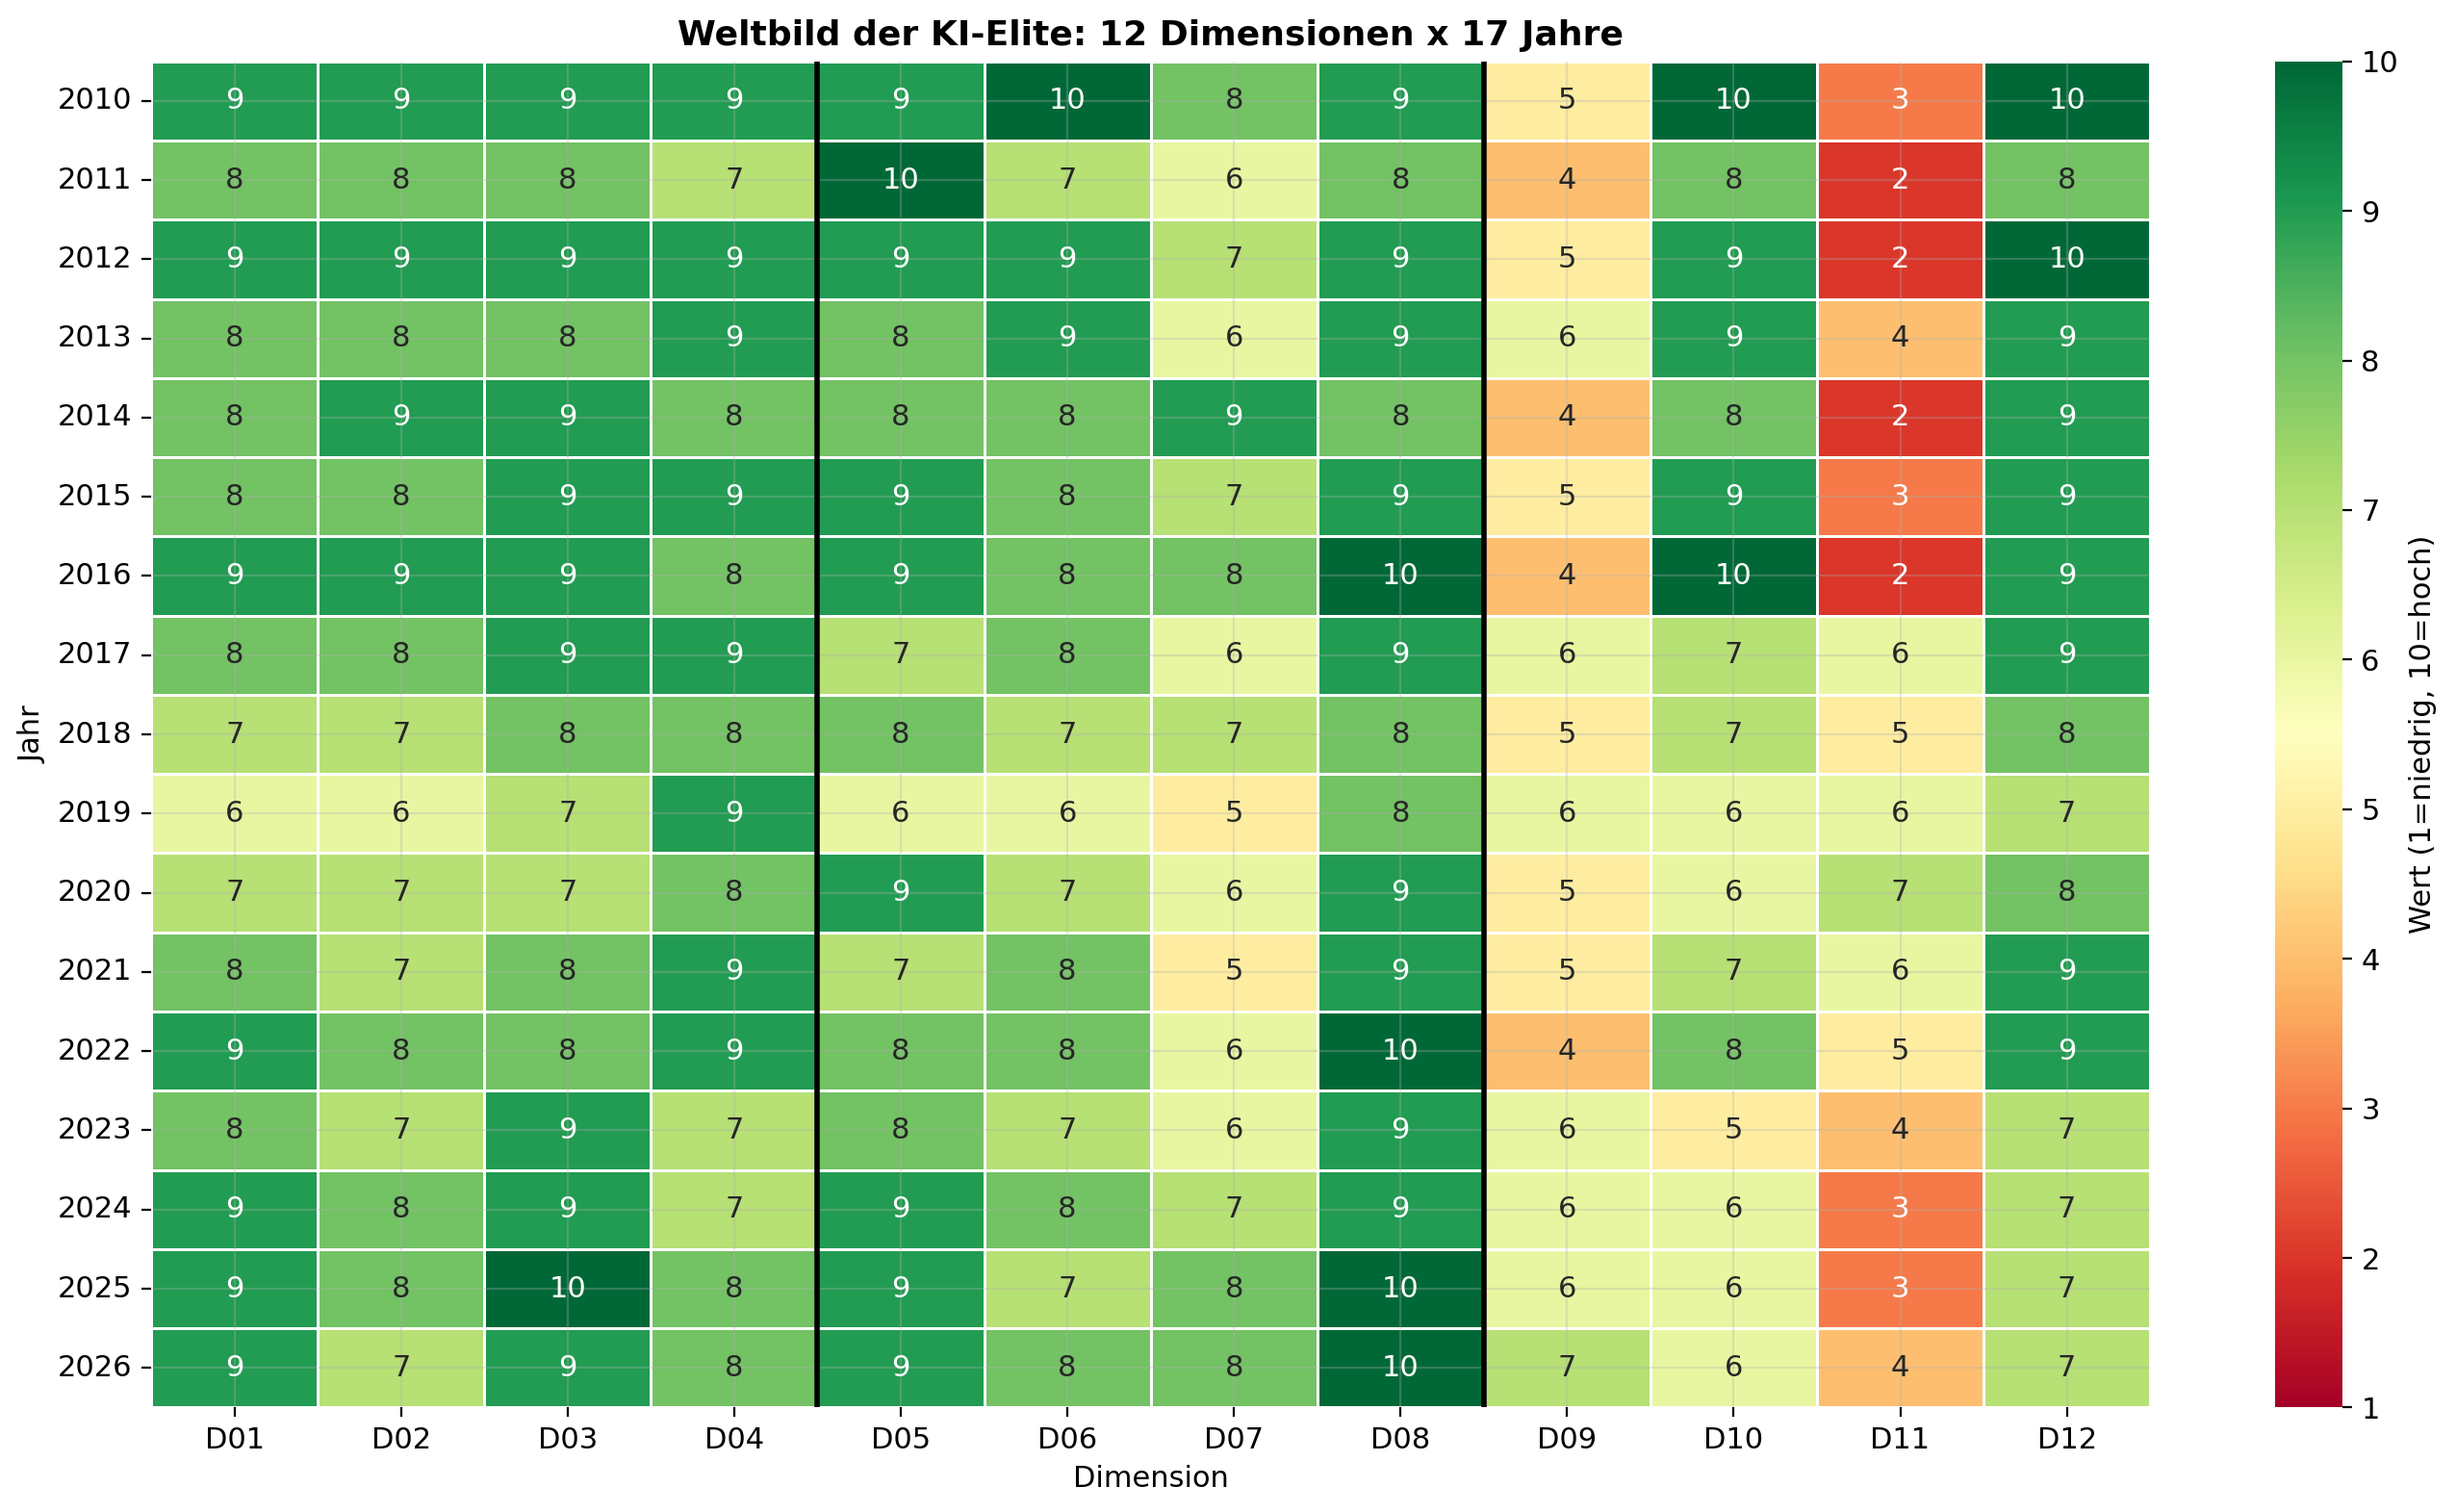
\includegraphics[width=0.95\textwidth]{fig2_heatmap.png}
  \caption{Heatmap der 12 Weltbild-Dimensionen über alle untersuchten Gruppen. Hohe Werte (dunkel) markieren intensive Überzeugungen; die Doppelsenke bei D09 und D11 ist über alle Gruppen hinweg sichtbar.}
  \label{fig:heatmap}
\end{figure}


\subsubsection{\texorpdfstring{Das Weltbild der Top~10}{Das Weltbild der Top 10}}

Die zehn mächtigsten KI-Akteure vertreten dasselbe Weltbild in intensivierter Form (Avg~7,7). Auf zehn von zwölf Dimensionen liegen die Top-10-Werte exakt einen Skalenpunkt über dem Kollektiv. Die beiden Ausnahmen: Menschenfreundlichkeit (D09=4) und Egalitarismus (D11=4) liegen \emph{niedriger}. Je mächtiger die Position, desto ausgeprägter das Sendungsbewusstsein und desto distanzierter das Menschenbild.


\subsubsection{Kernüberzeugungen}

Die Destillation der am häufigsten wiederholten Aussagen (SE~5: HOM\_haeuf\_A, vgl.\ Anhang~\ref{app:se}) identifiziert fünf Überzeugungen als Minimalkonsens: (1)~Technologie als moralisches Gebot, (2)~Elite-Steuerung, (3)~das Befreiungsnarrativ, (4)~geopolitischer Manichäismus, (5)~Arbeit als Identität. Sicherheitsrhetorik gehört zum Kernbestand des Diskurses, fungiert aber als diskursive Ressource, nicht als handlungsleitende Überzeugung.

\medskip
\noindent\textbf{Kernbefund F1:} Die rekonstruierten Profile deuten auf ein kohärentes, hochintensives Überzeugungssystem hin, das sich als \emph{technologischer Messianismus mit Ambivalenzstruktur} charakterisieren lässt. Die Bezeichnung \glqq Messianismus\grqq{} ist dabei als idealtypische Zuspitzung zu verstehen, nicht als psychologische Diagnose: Sie bezeichnet die spezifische \emph{Kombination} aus hohem Sendungsbewusstsein (D01), Techno-Determinismus (D05), Dringlichkeit (D08) und geringer anthropologischer Wertschätzung (D09) -- ein Profil, das über bloßes Sendungsbewusstsein hinausgeht, weil es technologischen Fortschritt als quasi-erlöserische Notwendigkeit rahmt.


\subsection{F2 -- Wandel des Weltbilds (längsschnittlich)}
\label{sec:ergebnisse:f2}

\subsubsection{Entwicklung der 12 Dimensionen über die Zeit}

Von zwölf Dimensionen zeigen vier ausgeprägte lineare Trends (Tabelle~\ref{tab:trends}).\footnote{Die hier berichteten Trendlinien beschreiben \textit{Muster in rekonstruierten Daten}: Die Weltbild-Werte sind LLM-gestützte Rekonstruktionen, keine unabhängigen Messungen. OLS-Steigungen und $R^2$ dienen der Beschreibung der Verlaufsmuster, nicht der inferenzstatistischen Hypothesenprüfung. Eine externe Validierung (Expertenratings vs.\ SWR-Output) steht noch aus (vgl.\ Abschnitt Limitations).}

\begin{table}[htbp]
  \centering
  \caption{Ausgeprägte lineare Trends (OLS-Beschreibung, $n=17$ Jahrespunkte).}
  \label{tab:trends}
  \begin{tabular}{l l c c}
    \toprule
    \textbf{Dimension} & \textbf{Richtung} & \textbf{Steigung/Dekade} & $R^2$ \\
    \midrule
    D10 Posthumanismus       & fallend  & $-2{,}4$ & $0{,}63$ \\
    \addlinespace[2pt]
    D12 Kontrollüberzeugung & fallend  & $-1{,}5$ & $0{,}54$ \\
    \addlinespace[2pt]
    D02 Selbstwirksamkeit    & fallend  & $-1{,}0$ & $0{,}31$ \\
    \addlinespace[2pt]
    D09 Menschenfreundlichkeit & steigend & $+0{,}9$ & $0{,}27$ \\
    \bottomrule
  \end{tabular}
\end{table}

Den stärksten Rückgang verzeichnet der Posthumanismus (D10): von 10 im Jahr 2010 auf 6 im Jahr 2025. Die hohe Spearman-Rangkorrelation mit D12 ($r_s = +0{,}85$)\footnote{Die hier und im Folgenden berichteten Korrelationen (Spearman-Rangkorrelationen, berechnet über die 17~Jahreszeitpunkte) sind \emph{Zusammenhänge innerhalb der LLM-Rekonstruktion}, nicht zwischen unabhängig gemessenen Variablen. Spearman wird verwendet, da die 12~Weltbild-Dimensionen Ordinalskalen darstellen; Pearson würde Intervallskalenniveau voraussetzen, das hier nicht gegeben ist. Die Korrelationen könnten interne Kohärenz des Modells widerspiegeln statt empirischer Zusammenhänge in der Realität (vgl.\ Abschnitt~\ref{sec:limitationen}).} weist auf ein zusammenhängendes Phänomen: Posthumanismus und Kontrollüberzeugung erodieren synchron. Der einzige deutlich steigende Wert betrifft die Menschenfreundlichkeit (D09), wobei die negative Korrelation mit D10 ($r_s = -0{,}58$) eine kompensatorische Verknüpfung nahelegt. Der Gesamtdurchschnitt bleibt nahezu konstant (Frühphase 7,5, Spätphase 7,3), was eine tektonische Verschiebung unter der Oberfläche verbirgt.

\begin{figure}[htbp]
  \centering
  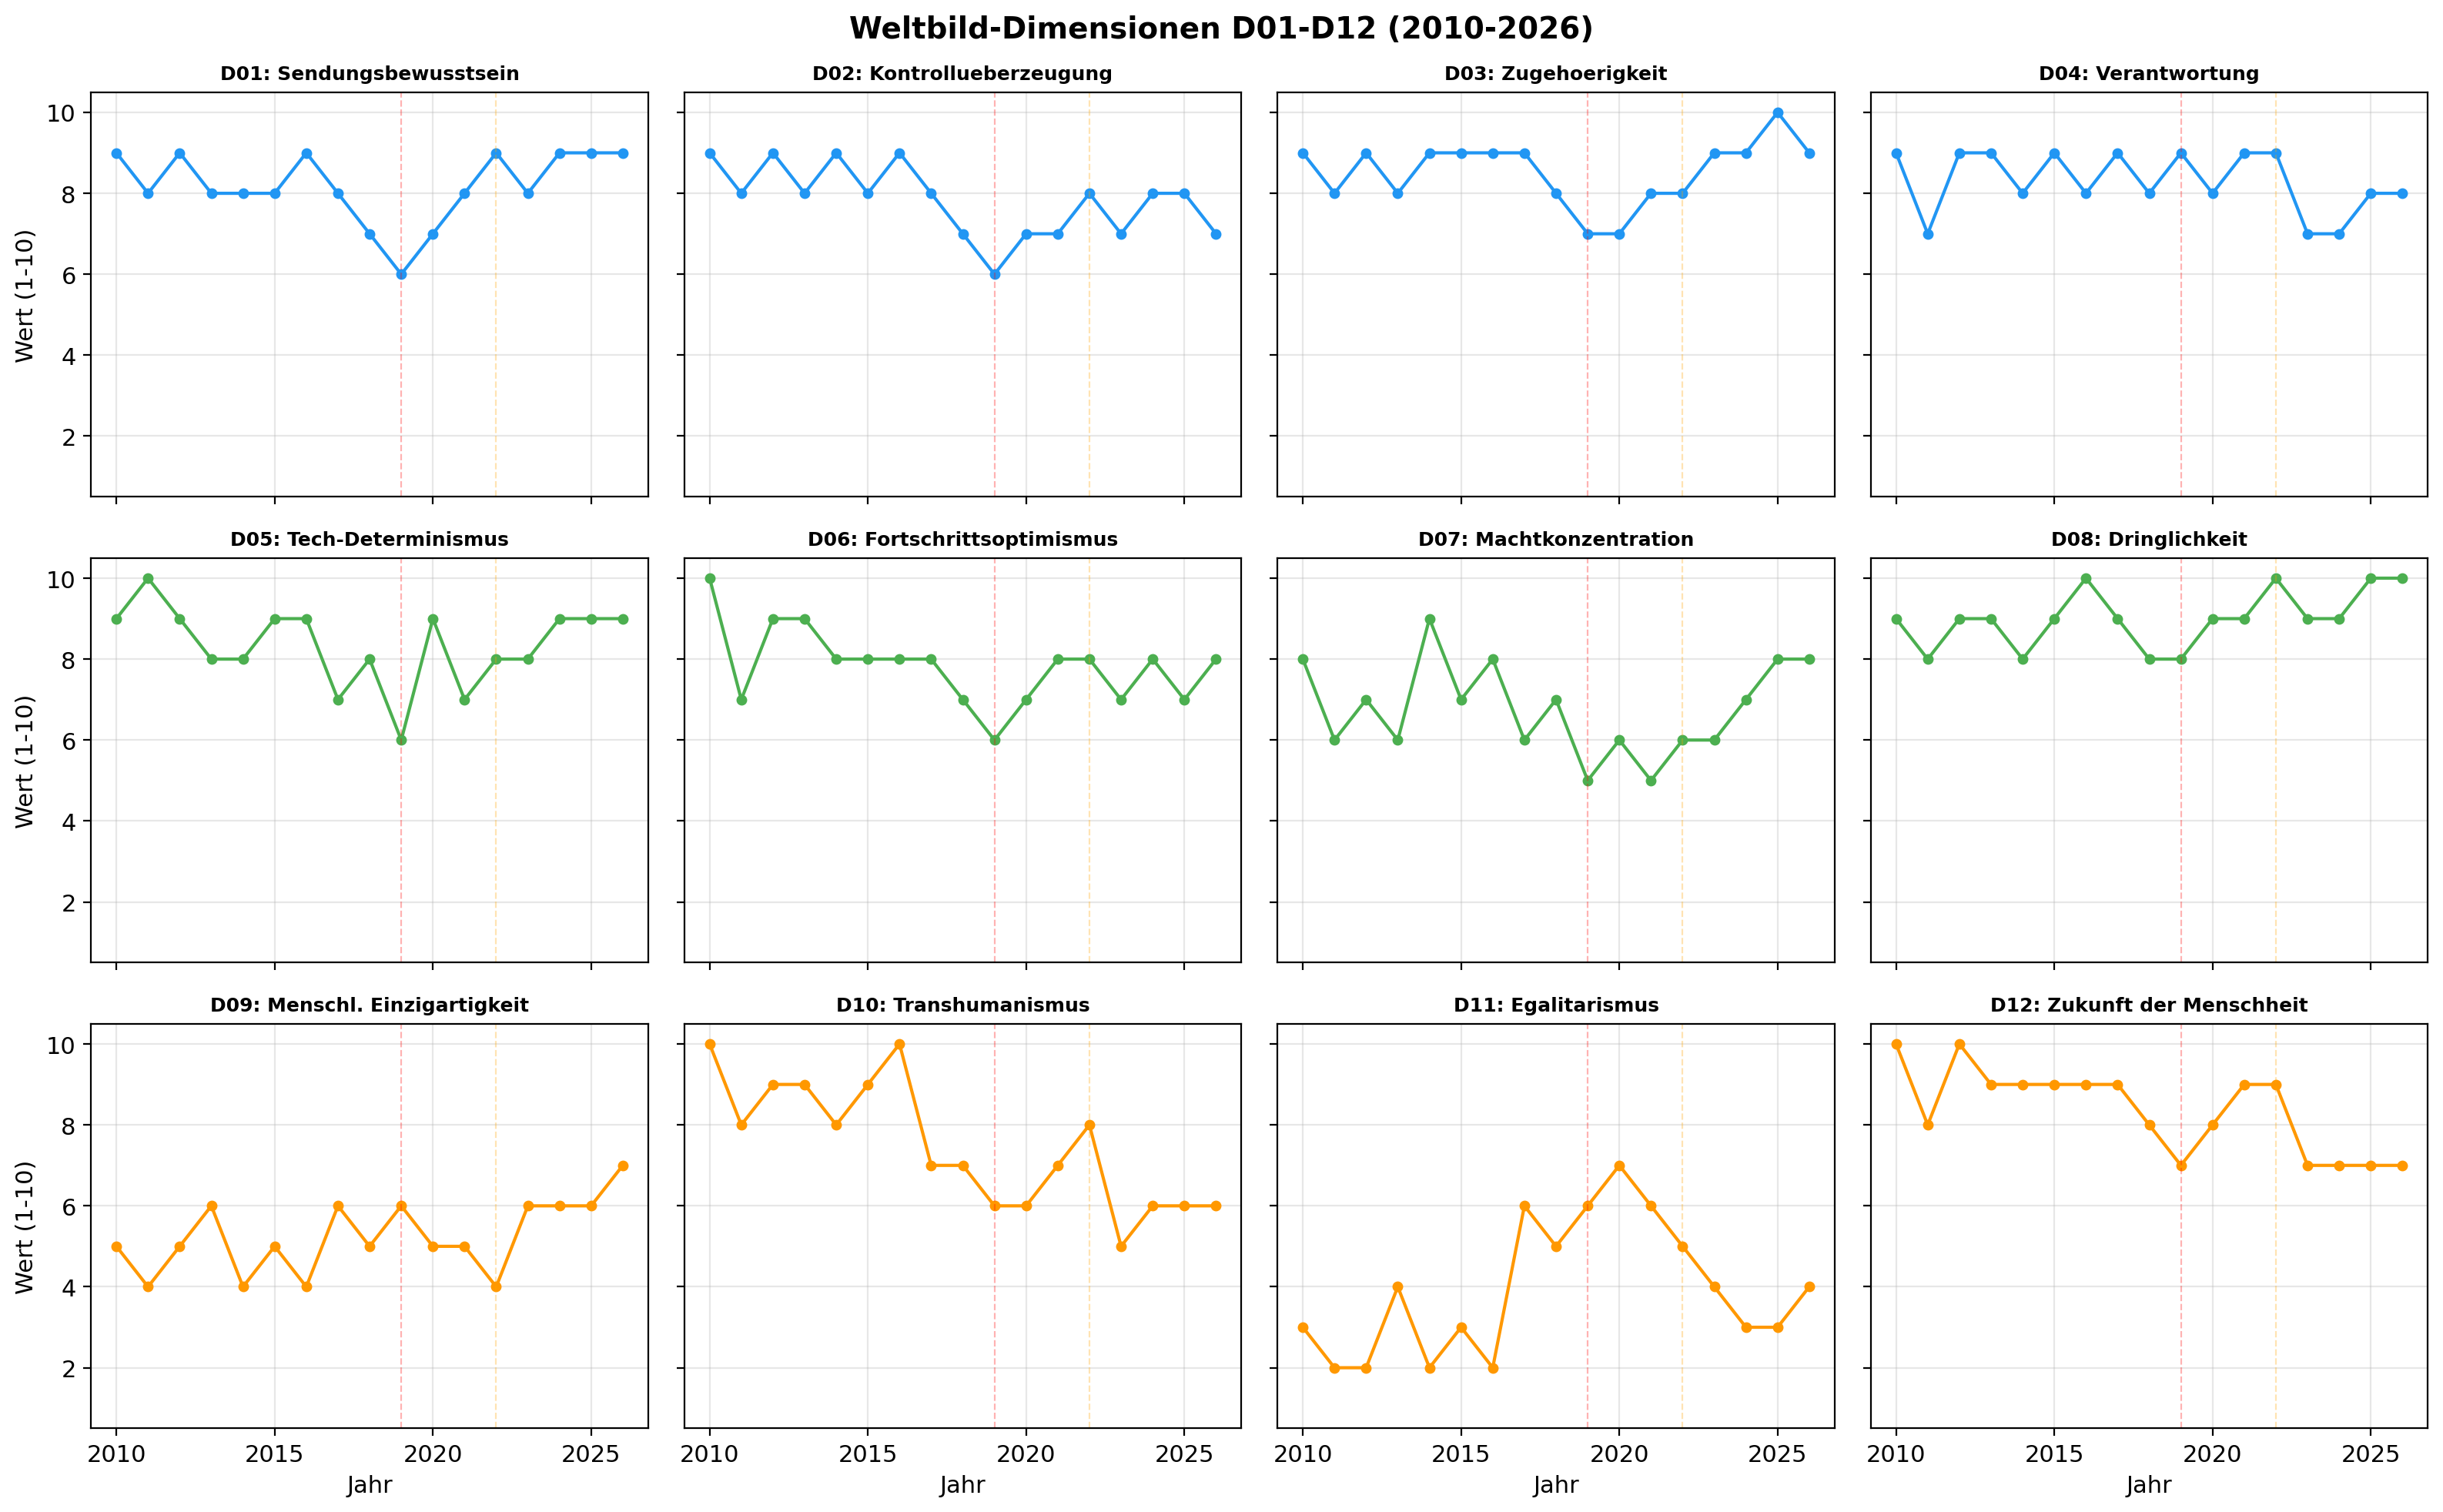
\includegraphics[width=\textwidth]{fig1_zeitreihen_panel.png}
  \caption{Zeitreihen der 12 Weltbild-Dimensionen (2010--2026). Ausgeprägte Trends sind hervorgehoben. Der markante Abfall von D10 (Posthumanismus) und D12 (Kontrollüberzeugung) bildet den \glqq Utopie-Komplex\grqq, dessen Zerfall durch steigende Dringlichkeit (D08) arithmetisch kompensiert wird.}
  \label{fig:zeitreihen}
\end{figure}

\begin{figure}[htbp]
  \centering
  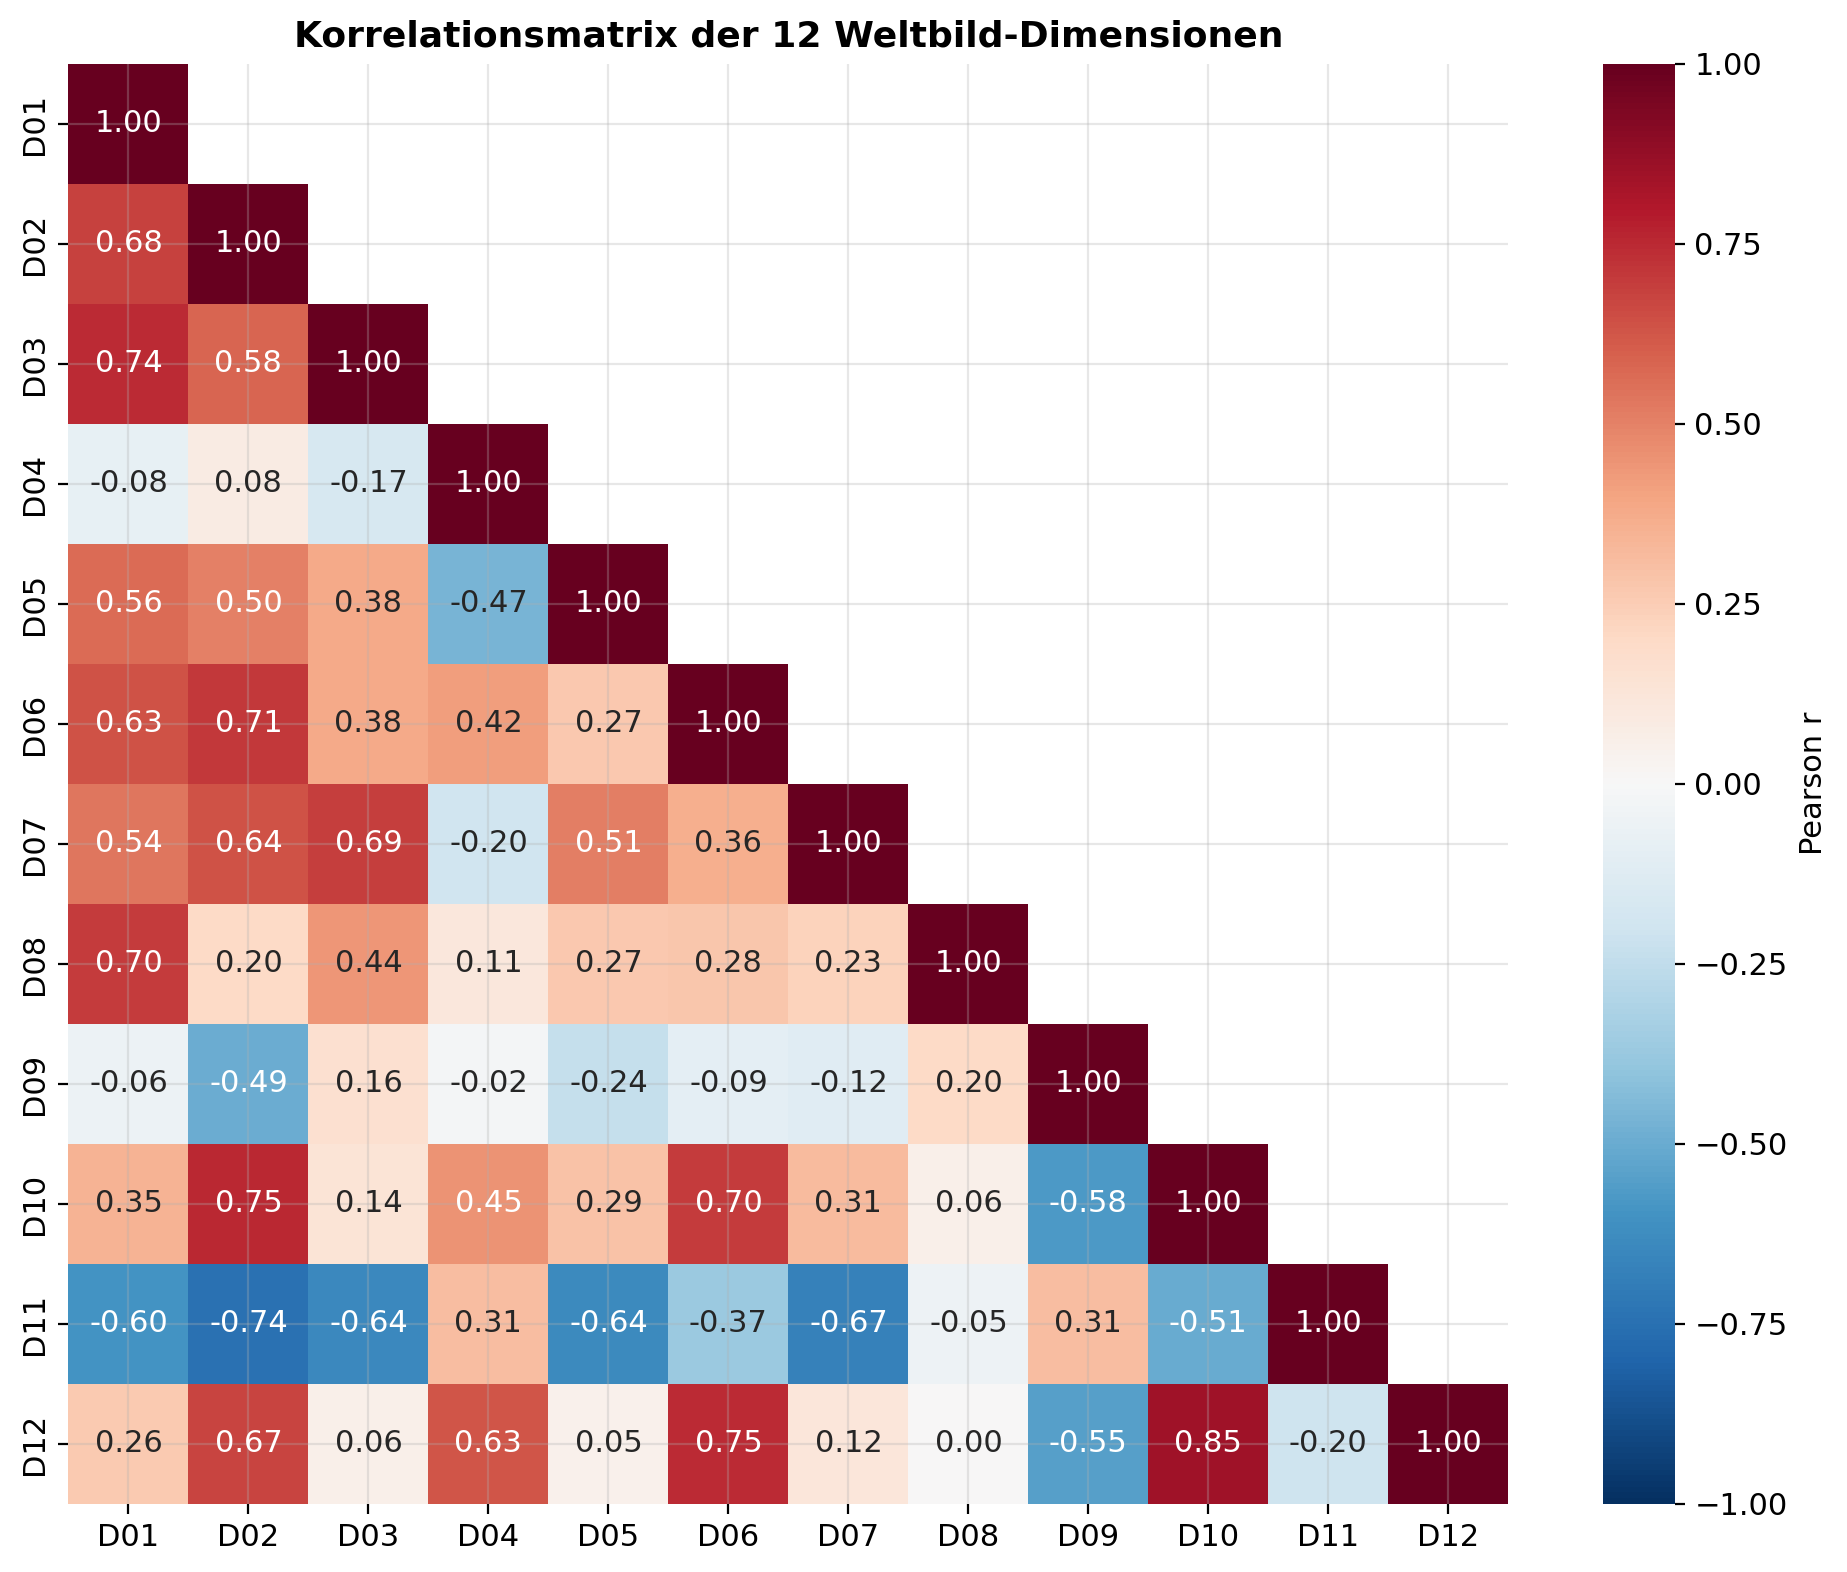
\includegraphics[width=0.85\textwidth]{fig4_korrelationsmatrix.png}
  \caption{Spearman-Rangkorrelationsmatrix der 12 Dimensionen. Die starke positive Korrelation zwischen D10 und D12 sowie die negative Korrelation zwischen D10 und D09 bilden den empirischen Kern des \glqq Utopie-Komplexes\grqq.}
  \label{fig:korrelationsmatrix}
\end{figure}


\subsubsection{Wendepunkte und Epochenvergleich}

Die Breakpoint-Detection -- durchgeführt als visuelle Inspektion der Zeitreihen, ergänzt durch die Identifikation synchroner Extrempunkte über mehrere Dimensionen -- identifiziert zwei zentrale Wendepunkte.\footnote{Eine formale Breakpoint-Analyse (z.\,B.\ Bai-Perron-Test) war aufgrund der geringen Zahl von Zeitpunkten ($n=17$) und der Natur der Daten (LLM-Rekonstruktionen, keine unabhängigen Messungen) nicht sinnvoll anwendbar. Die Wendepunkte sind daher als \emph{deskriptive Beobachtungen} zu verstehen, nicht als statistisch gesicherte Strukturbrüche.} Der erste liegt bei 2019: Vier Dimensionen (D01, D02, D05, D06) erreichen synchron ihren Tiefpunkt, zeitlich assoziiert mit der GPT-2-Zurückhaltung. Der zweite, dauerhaftere Wendepunkt liegt bei 2022/2023: Zeitgleich mit der ChatGPT-Veröffentlichung zeigt sich ein markanter Musterwechsel -- Dringlichkeit erreicht ihr rekonstruiertes Maximum (D08=10), Egalitarismus fällt von 6 auf 4. Im Unterschied zu 2019 kehren die Werte nicht zurück; die rekonstruierten Profile nach 2022 deuten auf ein neues Gleichgewicht hin. Dabei ist zu beachten, dass die identifizierten Wendepunkte nicht isoliert von breiteren gesellschaftlichen Entwicklungen zu sehen sind: Die COVID-19-Pandemie (2020--2022) hat die Digitalisierungsdynamik beschleunigt und dürfte das Dringlichkeitserleben verstärkt haben; die zunehmende geopolitische Polarisierung (US-China-Technologiekonflikt) hat den \glqq manichäischen\grqq{} Aspekt des Weltbilds möglicherweise befeuert; und der Beginn regulatorischer Initiativen (EU~AI~Act, 2021ff.) hat die Debatte um Governance verschärft. Diese Kontextfaktoren lassen sich mit der vorliegenden Methode nicht vom KI-spezifischen Wandel trennen.

\begin{figure}[htbp]
  \centering
  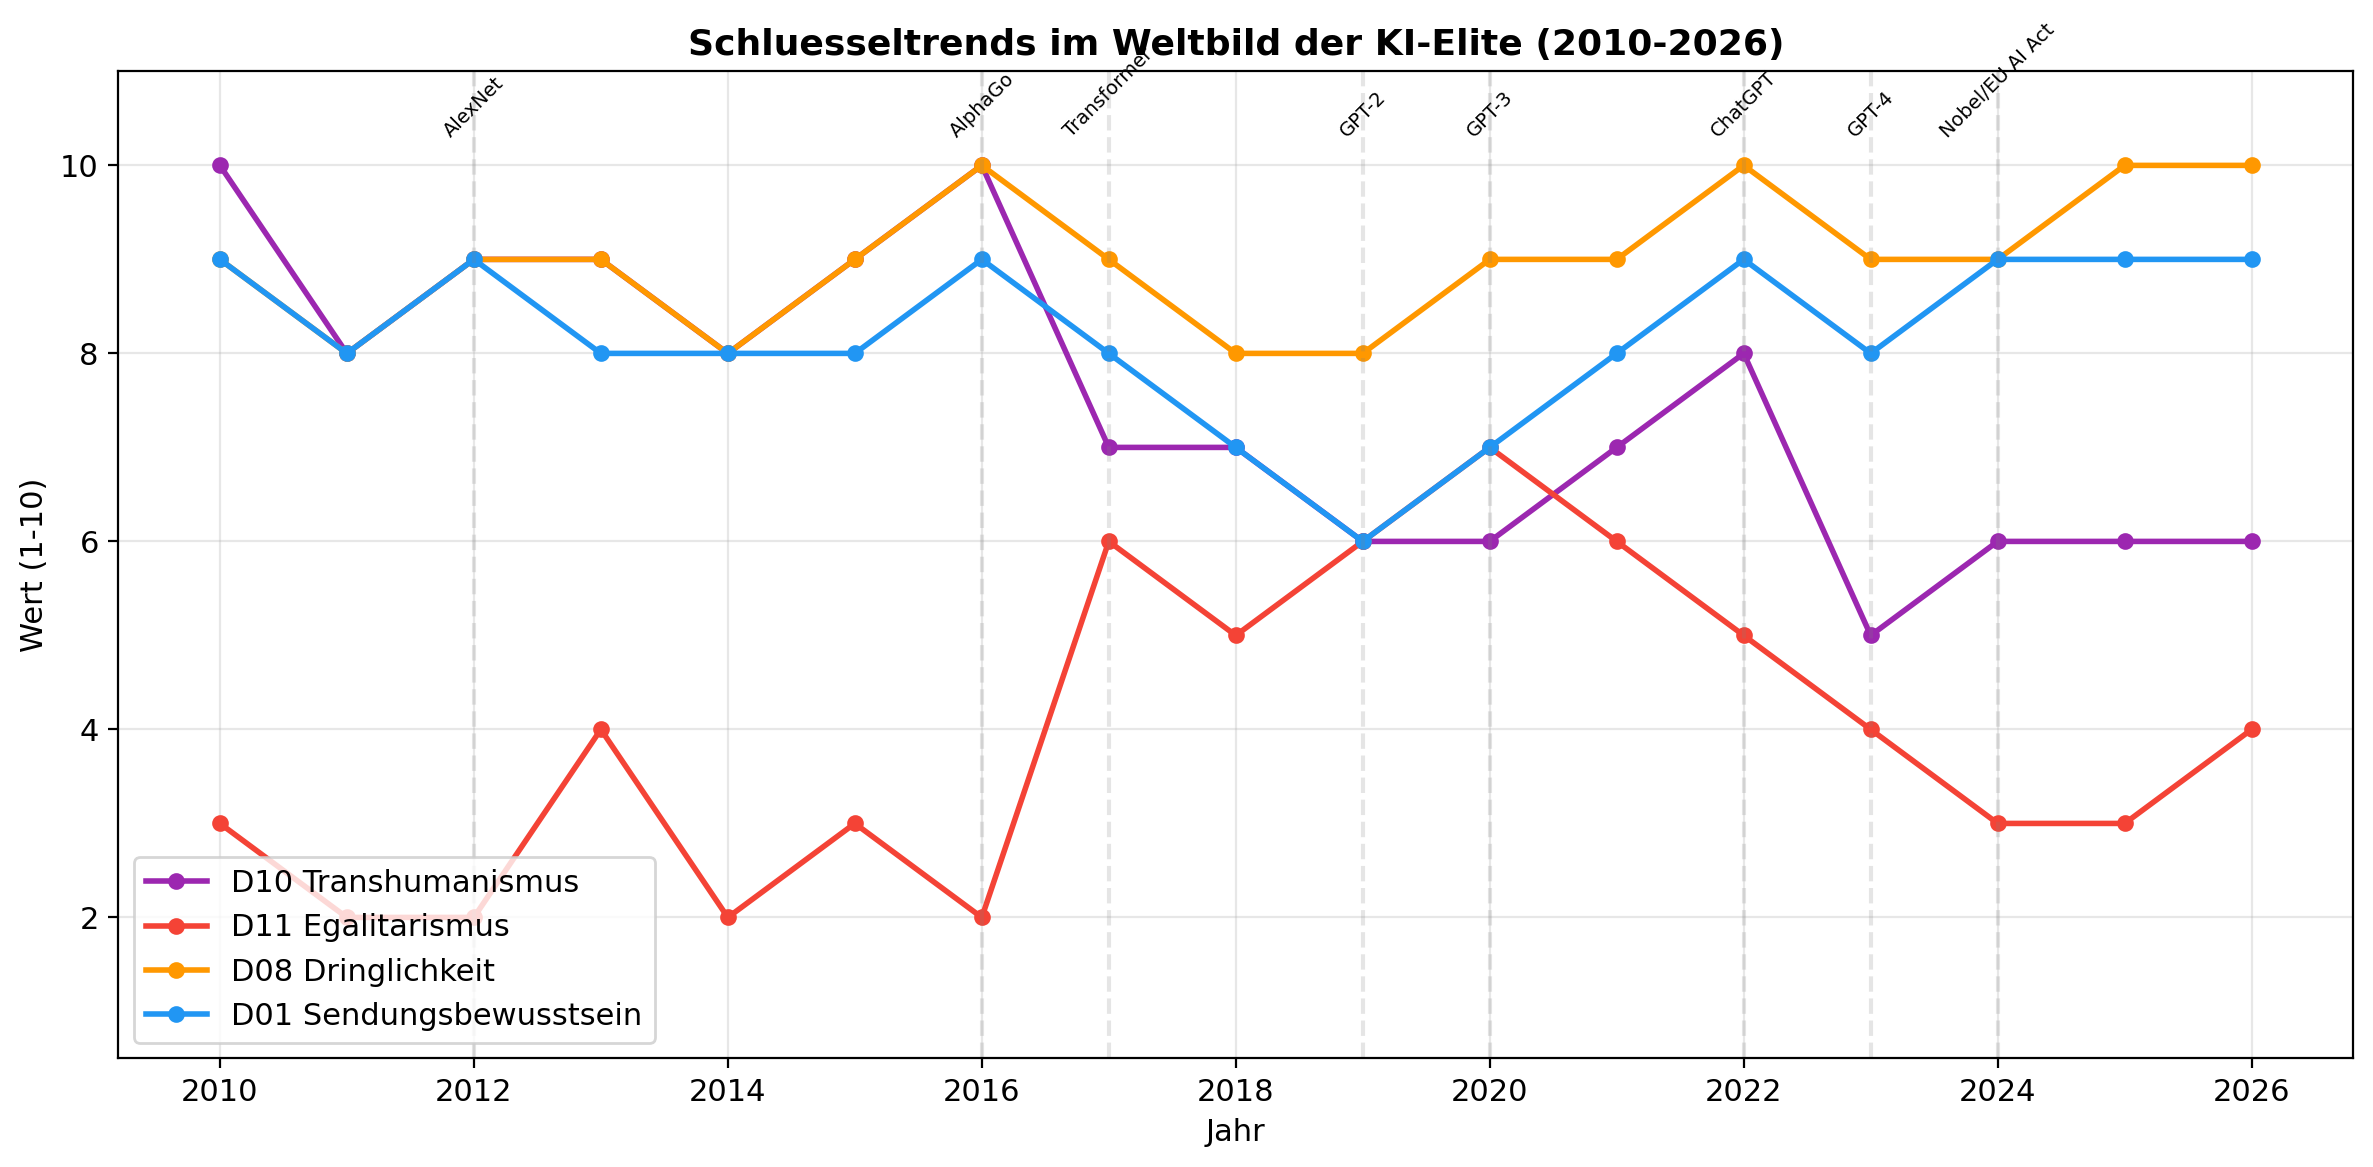
\includegraphics[width=0.95\textwidth]{fig7_schluesseltrends.png}
  \caption{Schlüsseltrends der Weltbild-Transformation. Die zwei Wendepunkte (2019, 2022/2023) und die drei Epochen (Prometheischer Optimismus, Erste Ambivalenz, Tragisches Bewusstsein) sind markiert.}
  \label{fig:schluesseltrends}
\end{figure}


\subsubsection{Konvergenz oder Divergenz?}

Die Daten zeigen eine zunehmende Ausdifferenzierung. Der ChatGPT-Effekt intensiviert sowohl die Architekten-Position (Beschleunigung, Machtkonzentration) als auch die Hüter-Position (Vorsicht, Regulierung) gleichzeitig -- er wirkt als Katalysator der Bipolarisierung.


\subsubsection{Metaphern- und Emotions-Wandel}

Die Leitmetapher verschiebt sich von Prometheus -- dem Feuerbringer -- zum tragischen Helden, der retten muss, was möglicherweise nicht mehr zu retten ist. Die Handlung bleibt dieselbe (Beschleunigung), aber ihre emotionale Rahmung dreht sich um: nicht mehr aus Euphorie, sondern aus dem Glauben, dass die Alternative schlimmer wäre.

\medskip
\noindent\textbf{Kernbefund F2:} Die rekonstruierten Profile deuten auf eine strukturelle Transformation des Weltbilds hin -- von einer monochromen Utopie zu einer bimodalen Wette. \emph{Tragisch} im Sinne der Bezeichnung \glqq tragischer Beschleunigungszwang\grqq{} meint die gleichzeitige Erosion utopischer Gewissheiten und Persistenz der Handlungsrichtung: Die Akteure beschleunigen, obwohl sie an der Zukunft zweifeln, die sie bauen -- weil sie die Alternativen (geopolitischer Rückfall, Kontrollverlust an weniger verantwortungsvolle Akteure) als schlimmer bewerten. Drei Erosionstrends (D10, D12, D02) bilden einen \glqq Utopie-Komplex\grqq, dessen Zerfall durch steigende Dringlichkeit (D08) arithmetisch kompensiert wird. Allerdings ist nicht auszuschließen, dass der Rückgang des Posthumanismus (D10) teilweise ein Artefakt veränderter öffentlicher Diskurse ist: Wenn das Thema medial weniger präsent ist, sinkt auch die Datendichte entsprechender Aussagen, was die LLM-Rekonstruktion verzerren kann.


\subsection{F3 -- Kongruenz von Aussagen und Handlungen}
\label{sec:ergebnisse:f3}

\begin{table}[htbp]
  \centering
  \caption{Vergleich Aussagen (A) und Handlungen (H), $N=100$. Werte sind Einzel-Run-Ratings auf Gruppenebene (v2, mit strikter Instanztrennung). v1-Werte (Same-Instance-Ratings) zum Vergleich.}
  \label{tab:kongruenz}
  \begin{tabular}{l c c c c c}
    \toprule
    \textbf{Dimension} & \textbf{Sagen v2} & \textbf{Handeln v2} & $\Delta$\textbf{v2} & $\Delta$\textbf{v1} & \textbf{Stabil?} \\
    \midrule
    \multicolumn{6}{l}{\textit{Selbstbild (AV1)}} \\
    D01 Sendungsbewusstsein     & 9 & 9 & $0$  & $-1$ & -- \\
    D02 Selbstwirksamkeit       & 8 & 9 & $+1$ & $+1$ & \checkmark \\
    D03 Arbeitsethos            & 9 & 9 & $0$  & $+1$ & -- \\
    D04 Verantwortungsgefühl  & 8 & 8 & $0$  & $-2$ & -- \\
    \addlinespace[3pt]
    \multicolumn{6}{l}{\textit{Weltbild (AV2)}} \\
    D05 Techno-Determinismus    & 7 & 9 & $\mathbf{+2}$ & $+1$ & $\uparrow$ \\
    D06 Fortschrittsglaube      & 8 & 8 & $0$  & $-1$ & -- \\
    D07 Machtkonzentration      & 6 & 8 & $\mathbf{+2}$ & $+2$ & \checkmark\checkmark \\
    D08 Dringlichkeit           & 9 & 9 & $0$  & $+1$ & -- \\
    \addlinespace[3pt]
    \multicolumn{6}{l}{\textit{Menschenbild (AV3)}} \\
    D09 Menschenfreundlichkeit  & 6 & 5 & $-1$ & $-2$ & $\downarrow$ \\
    D10 Posthumanismus          & 7 & 7 & $0$  & $+1$ & -- \\
    D11 Egalitarismus           & 5 & 3 & $\mathbf{-2}$ & $-3$ & \checkmark\checkmark \\
    D12 Kontrollüberzeugung   & 7 & 8 & $+1$ & $-1$ & -- \\
    \midrule
    \textbf{Durchschnitt}       & \textbf{7,4} & \textbf{7,7} & $+0{,}3$ & $-0{,}4$ & \\
    MAE                         &   &   & $0{,}75$ & $1{,}42$ & \\
    \bottomrule
  \end{tabular}
\end{table}

\noindent\textbf{Methodische Anmerkung:} Die v1-Ratings (in früheren Versionen dieser Studie berichtet) wurden innerhalb derselben LLM-Instanz generiert, wodurch Kreuzkontamination zwischen Aussagen- und Handlungsprofilen möglich war. Die hier gezeigten v2-Ratings verwenden strikte Instanztrennung: Jeder Datentyp wurde von einem unabhängigen Agenten ohne Zugang zum anderen verarbeitet. Dies reduzierte die Gesamtkluft von MAE $= 1{,}42$ auf MAE $= 0{,}75$ ($-47\,\%$), und die v2-Kluft fällt unter die Kontrollbaseline (G6~v2: MAE $= 0{,}92$). Das bedeutet: Die \emph{Gesamt}-Sagen-Handeln-Kluft ist in Einzeldurchläufen nicht zuverlässig vom Messrauschen unterscheidbar.

Allerdings zeigen zwei spezifische Dimensionen \emph{stabile} Diskrepanzen über beide Messbedingungen: \textbf{D07 Machtkonzentration} ($\Delta = +2$ in v1 und v2) und \textbf{D11 Egalitarismus} ($\Delta = -2$ in v2, $-3$ in v1). Diese bilden die robusten Sagen-Handeln-Befunde der Studie. Handlungen konzentrieren Macht stärker als die Rhetorik nahelegt, und Handlungen sind weniger egalitär als die Rhetorik behauptet. Beides ist konsistent mit einer strukturellen \emph{Erwünschtheits-Asymmetrie}: Der öffentliche Diskurs überschätzt egalitäre und demokratische Commitments relativ zum operativen Verhalten.

\begin{figure}[htbp]
  \centering
  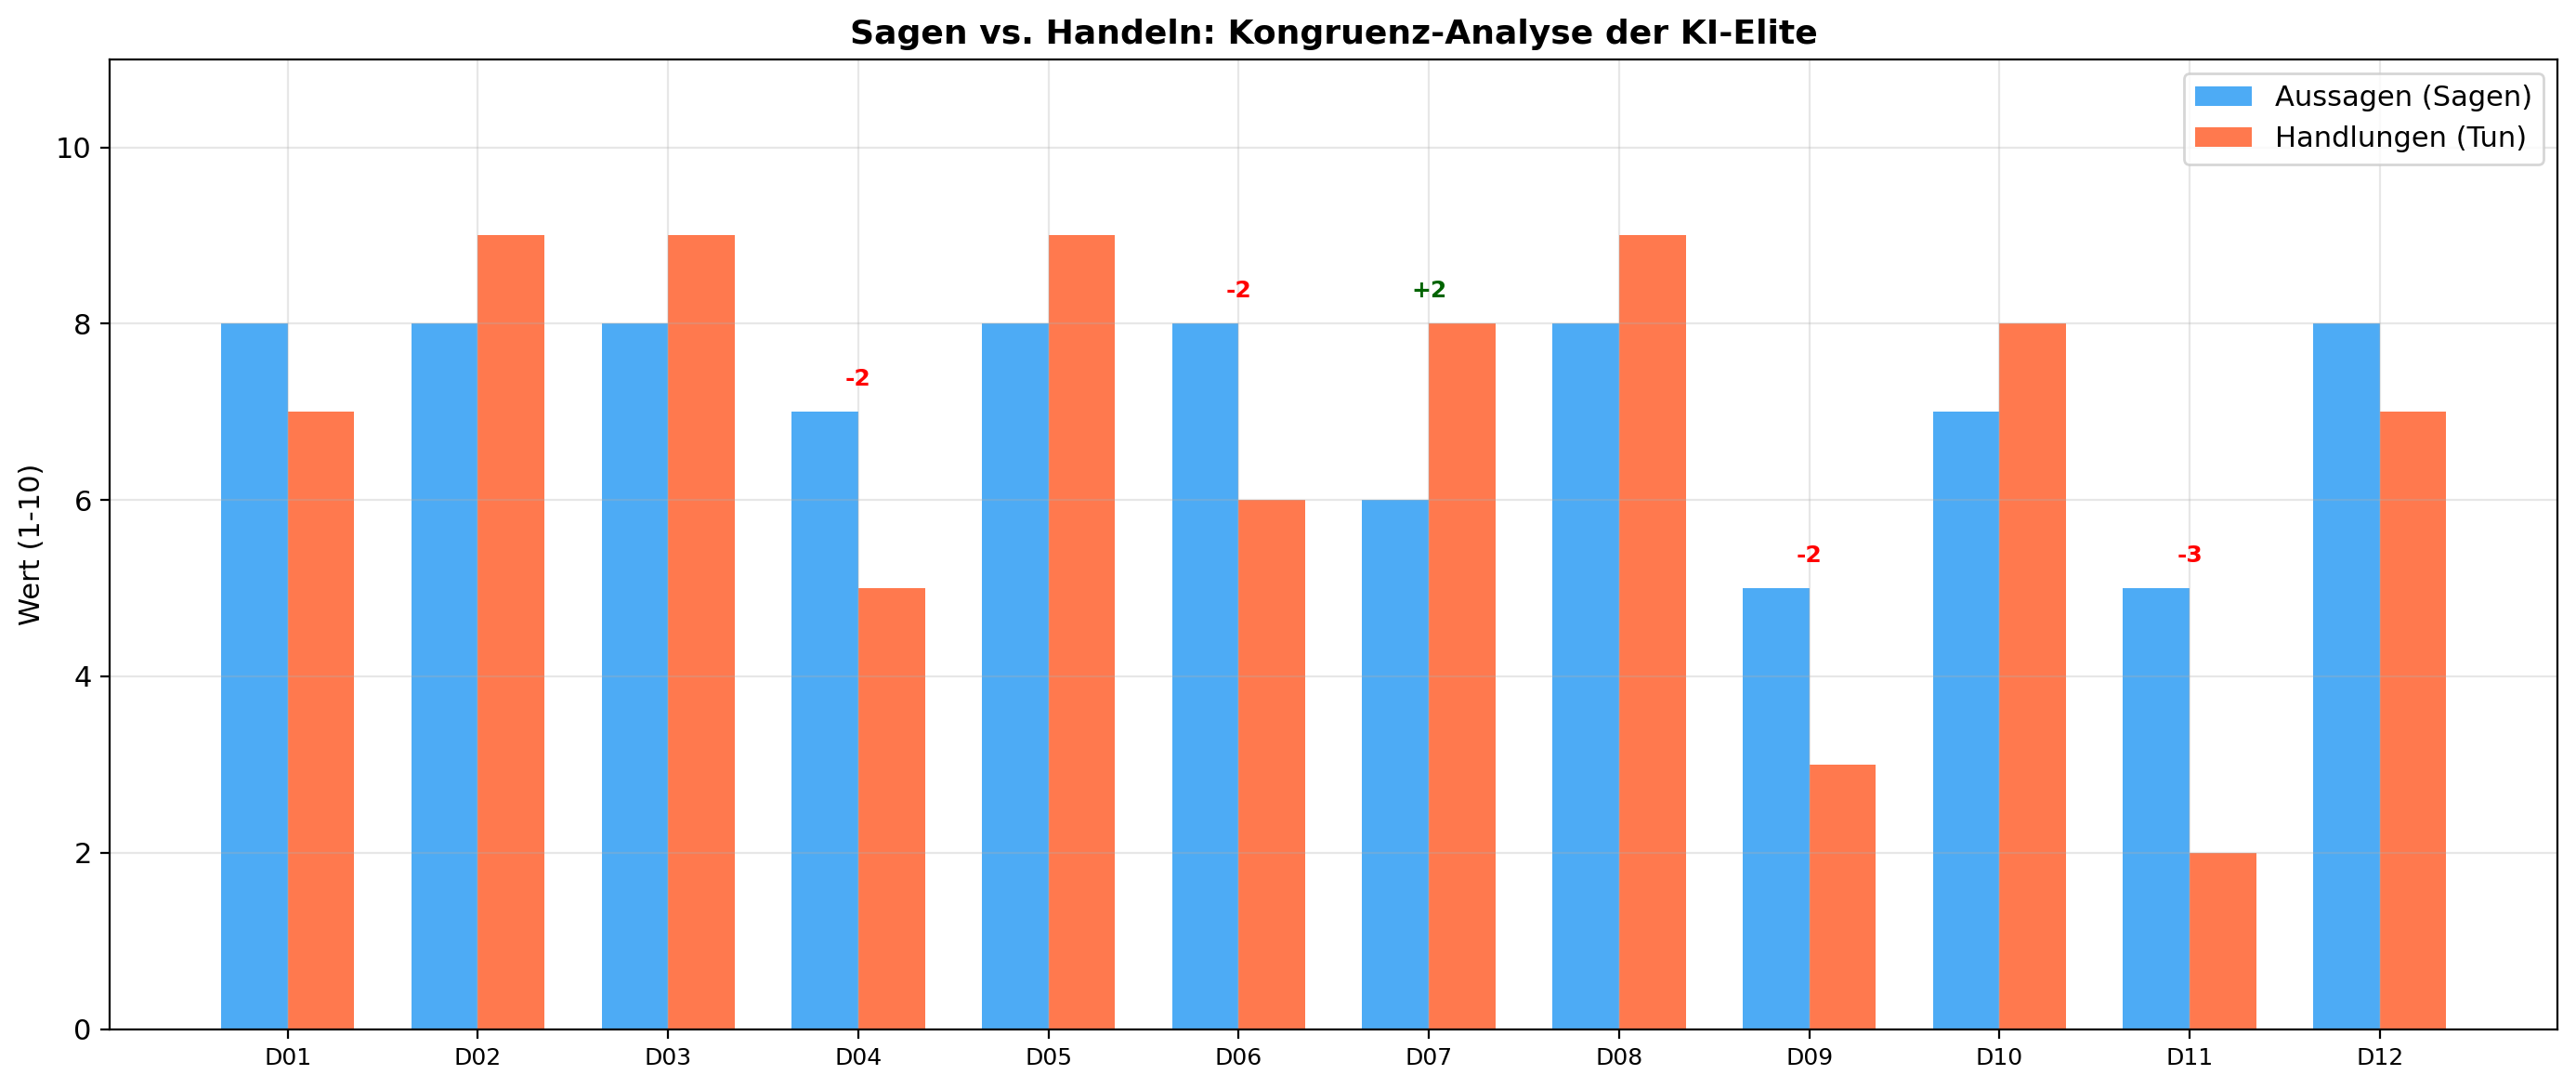
\includegraphics[width=0.95\textwidth]{fig6_sagen_vs_handeln.png}
  \caption{Sagen vs.\ Handeln: Vergleich der aus Aussagen (A) und Handlungen (H) rekonstruierten Weltbilder. Die gesellschaftsorientierten Dimensionen (D04, D06, D09, D11) fallen im Handeln systematisch ab, während die machtbezogenen Dimensionen (D07, D05) im Handeln steigen.}
  \label{fig:sagen_handeln}
\end{figure}

Die größte stabile Einzeldiskrepanz (D11, $\Delta\,-2$ in v2, $-3$ in v1) zeigt: In Aussagen spricht die KI-Elite von \glqq Zugang für alle\grqq; in ihren Handlungen baut sie Mehrfach-Stimmrechtsaktien, konzentriert Compute-Infrastruktur und schafft exklusive Netzwerke. D07 (Machtkonzentration, $\Delta\,+2$) ist der komplementäre Befund: Die Rhetorik favorisiert verteilte Governance, aber operative Entscheidungen zentralisieren Kontrolle.

\subsubsection{Gruppen-Dekomposition der Sagen-Handeln-Kluft}

Der aggregierte Sagen-Handeln-Vergleich verdeckt substanzielle gruppenspezifische Variation -- ein Simpson-Paradoxon. Wenn fünf soziologische Gruppen mit strikter Instanztrennung analysiert werden (Aussagen- und Handlungskorpus von unabhängigen Agenten verarbeitet), emergieren drei distinkte Muster:

\begin{itemize}
\item \textbf{CEOs} (MAE $= 1{,}08$, über Baseline): Die klassische Erwünschtheitslücke. Rhetorik ist egalitärer (D11: Sagen~5, Handeln~3, $\Delta = -2$) und weniger machtkonzentrierend (D07: Sagen~7, Handeln~9, $\Delta = +2$) als operatives Verhalten. CEOs sagen das \glqq Richtige\grqq{} über verteilte Governance und bauen gleichzeitig Dual-Class-Aktienstrukturen.

\item \textbf{Risiko-Warner} (MAE $= 1{,}92$, stärkste Kluft): Keine inverse Kluft, sondern \emph{prophetische Konsistenz}. Bei Dekomposition nach abhängiger Variable wird das Muster klar: DV1 (Selbstbild, D01--D04) zeigt nahezu perfekte Konsistenz (MAE $= 0{,}8$) -- Risiko-Warner wissen, wer sie sind. Die Diskrepanz konzentriert sich in DV3 (Menschenbild, MAE $= 3{,}2$): Ihre \emph{Aussagen} beschreiben eine gefürchtete Zukunft -- Mensch als ersetzbar (D09: Sagen~4), posthumanistische Transformation als unvermeidlich (D10: Sagen~9) -- während ihre \emph{Handlungen} ihre tatsächlichen Werte offenbaren: hohe Menschenfreundlichkeit (D09: Handeln~8), Ablehnung des Posthumanismus in der Praxis (D10: Handeln~4), aktive Handlungsfähigkeit (D12: Handeln~8). Dies ist die Struktur prophetischer Warnung: eine Möglichkeitsprojektion artikulieren, die man \emph{verhindern} will, und dann konsequent dagegen handeln. Ihre Sagen-Handeln-Kluft ist keine Heuchelei, sondern die Signatur antizipatorischer Ethik -- ein Befund, der ohne Gruppendekomposition unsichtbar bliebe.

\item \textbf{Investoren} (MAE $= 0{,}75$, unter Baseline): Die konsistenteste Gruppe. Rhetorik und Handeln erzählen dieselbe Geschichte: radikaler Techno-Optimismus mit minimaler egalitärer Orientierung. Keine Erwünschtheitslücke -- sie meinen, was sie sagen.

\item \textbf{Beschleuniger} (MAE $= 0{,}92$, an Baseline): Ein Grenzmuster, das einer schwächeren Version der CEO-Erwünschtheitslücke ähnelt. Rhetorik ist optimistischer hinsichtlich Fortschritt (D06: $\Delta = -2$), verantwortungsvoller (D04: $\Delta = -2$) und egalitärer (D11: $\Delta = -2$) als operatives Verhalten.
\end{itemize}

\noindent Diese entgegengesetzten gruppenspezifischen Klüfte heben sich im Aggregat auf (Gesamt-MAE $= 0{,}75$, unter der G6-v2-Kontrollbaseline von $0{,}92$). Die Sagen-Handeln-Kluft ist nicht absent -- sie ist \emph{gruppenspezifisch und richtungsabhängig} und erfordert Dekomposition statt aggregierter Berichterstattung.

\medskip
\noindent\textbf{Kernbefund F3:} Zwei robuste Sagen-Handeln-Diskrepanzen überstehen die Instanztrennung: D07~(Machtkonzentration) und D11~(Egalitarismus). Die Gesamtmagnitude der Kluft ist messbedingt variabel und sollte in Einzeldurchläufen nicht überinterpretiert werden. Aber die \emph{Richtung} der Asymmetrie ist stabil: Der öffentliche Diskurs ist egalitärer und machtverteilender als das operative Verhalten. Eine formale Quantifizierung (mit Konfidenzintervallen aus $N \geq 30$ wiederholten Messungen) bleibt ein Desiderat.


\subsection{F4 -- Weltbild-Cluster}
\label{sec:ergebnisse:f4}

Aus den Daten lassen sich vier distinkte Weltbild-Typen identifizieren (Tabelle~\ref{tab:typen}).

\textbf{Identifikationsmethode:} Die Cluster-Identifikation erfolgte in einem zweistufigen Verfahren. \emph{Stufe~1 (LLM-gestützt):} Alle 15 Gruppen-Synthesen wurden nach Ähnlichkeitsmustern in den 12~Dimensionen gruppiert, wobei die größten Varianzachsen (D07~Machtkonzentration, D09~Menschenfreundlichkeit, D11~Egalitarismus) als Trennmerkmale fungierten. \emph{Stufe~2 (Autor-Validierung):} Die vom LLM vorgeschlagene Vier-Cluster-Lösung wurde vom Autor anhand inhaltlicher Kohärenz und Plausibilität evaluiert. Alternative Lösungen (drei und fünf Cluster) wurden geprüft und verworfen: Drei Cluster verschmelzen Innovator und Befreier, was inhaltlich nicht gerechtfertigt ist; fünf Cluster spalten den Hüter-Typ in eine Untergruppe, die empirisch nicht stabil reproduziert werden konnte. Wir betonen, dass diese Cluster-Identifikation \emph{explorativ} ist -- eine konfirmatorische Validierung an einem unabhängigen Datensatz steht aus. Die Cluster-Lösung ist eine \emph{interpretative Hypothese}, nicht ein statistisch abgesichertes Ergebnis im Sinne formaler Clusteranalyse.

\begin{table}[htbp]
  \centering
  \caption{Die vier Weltbild-Typen der KI-Elite. Die Werte sind Cluster-Durchschnitte aus den Gruppen-Synthesen; individuelle Abweichungen innerhalb eines Clusters können erheblich sein (vgl.\ die Andreessen-Diskrepanz in der nachfolgenden Fußnote).}
  \label{tab:typen}
  \small
  \resizebox{\textwidth}{!}{%
  \begin{tabular}{l c c c c}
    \toprule
    \textbf{Merkmal} & \textbf{I \glqq Architekt\grqq} & \textbf{II \glqq Hüter\grqq} & \textbf{III \glqq Innovator\grqq} & \textbf{IV \glqq Befreier\grqq} \\
    \midrule
    $n$ & 35 & 25 & 22 & 18 \\
    \addlinespace[2pt]
    Prototyp & CEOs, Investoren & Akademiker, Risiko-W. & Gründer & Open Source \\
    \addlinespace[2pt]
    Avg D01--D12 & 7,8 & 6,4 & 7,2 & 6,8 \\
    \midrule
    D04 Verantwortung & 6,3 & \textbf{9,0} & 8,3 & 6,0 \\
    \addlinespace[2pt]
    D07 Machtkonzentr. & \textbf{8,8} & 4,8 & 6,5 & \textbf{2,5} \\
    \addlinespace[2pt]
    D09 Menschenfreundl. & \textbf{3,3} & 5,8 & 4,8 & \textbf{6,5} \\
    \addlinespace[2pt]
    D11 Egalitarismus & \textbf{2,8} & \textbf{7,2} & 5,0 & \textbf{7,5} \\
    \bottomrule
  \end{tabular}%
  }
\end{table}

Der \textbf{Architekt} vereint maximales Sendungsbewusstsein mit minimalem Egalitarismus: Machtkonzentration ist Voraussetzung für Handlungsfähigkeit. Der \textbf{Hüter} bildet den Gegenpol: maximale Verantwortung, Forderung nach institutioneller Begrenzung. Der \textbf{Innovator} steht dazwischen. Der \textbf{Befreier} ist die überraschendste Entdeckung: minimale Machtkonzentration \emph{und} hoher Egalitarismus -- Regulierungsgegner, die Macht radikaler verteilen wollen als alle anderen, allerdings durch Märkte und Open-Source-Communities.\footnote{Der hohe D11-Wert des Befreier-Typs (7,5) und der niedrige D11-Wert einzelner Prototypen (z.\,B.\ Andreessen: D11=2) markieren eine Konstruktvaliditätsproblem: D11 misst Gleichheitsorientierung, nicht deren \emph{Mechanismus}. Marktlibertaerer Zugangs-Egalitarismus (Befreier) und redistributiver Egalitarismus (Hüter) produzieren ähnliche Skalenwerte auf D11, meinen aber Verschiedenes. Der Prototyp-Wert bezieht sich auf die Einzelperson-Synthese, der Cluster-Wert auf das Gruppenaggregat -- Andreessens individuelles Profil weicht vom Cluster-Durchschnitt ab. Künftige Operationalisierungen sollten hier differenzieren.}

\begin{figure}[htbp]
  \centering
  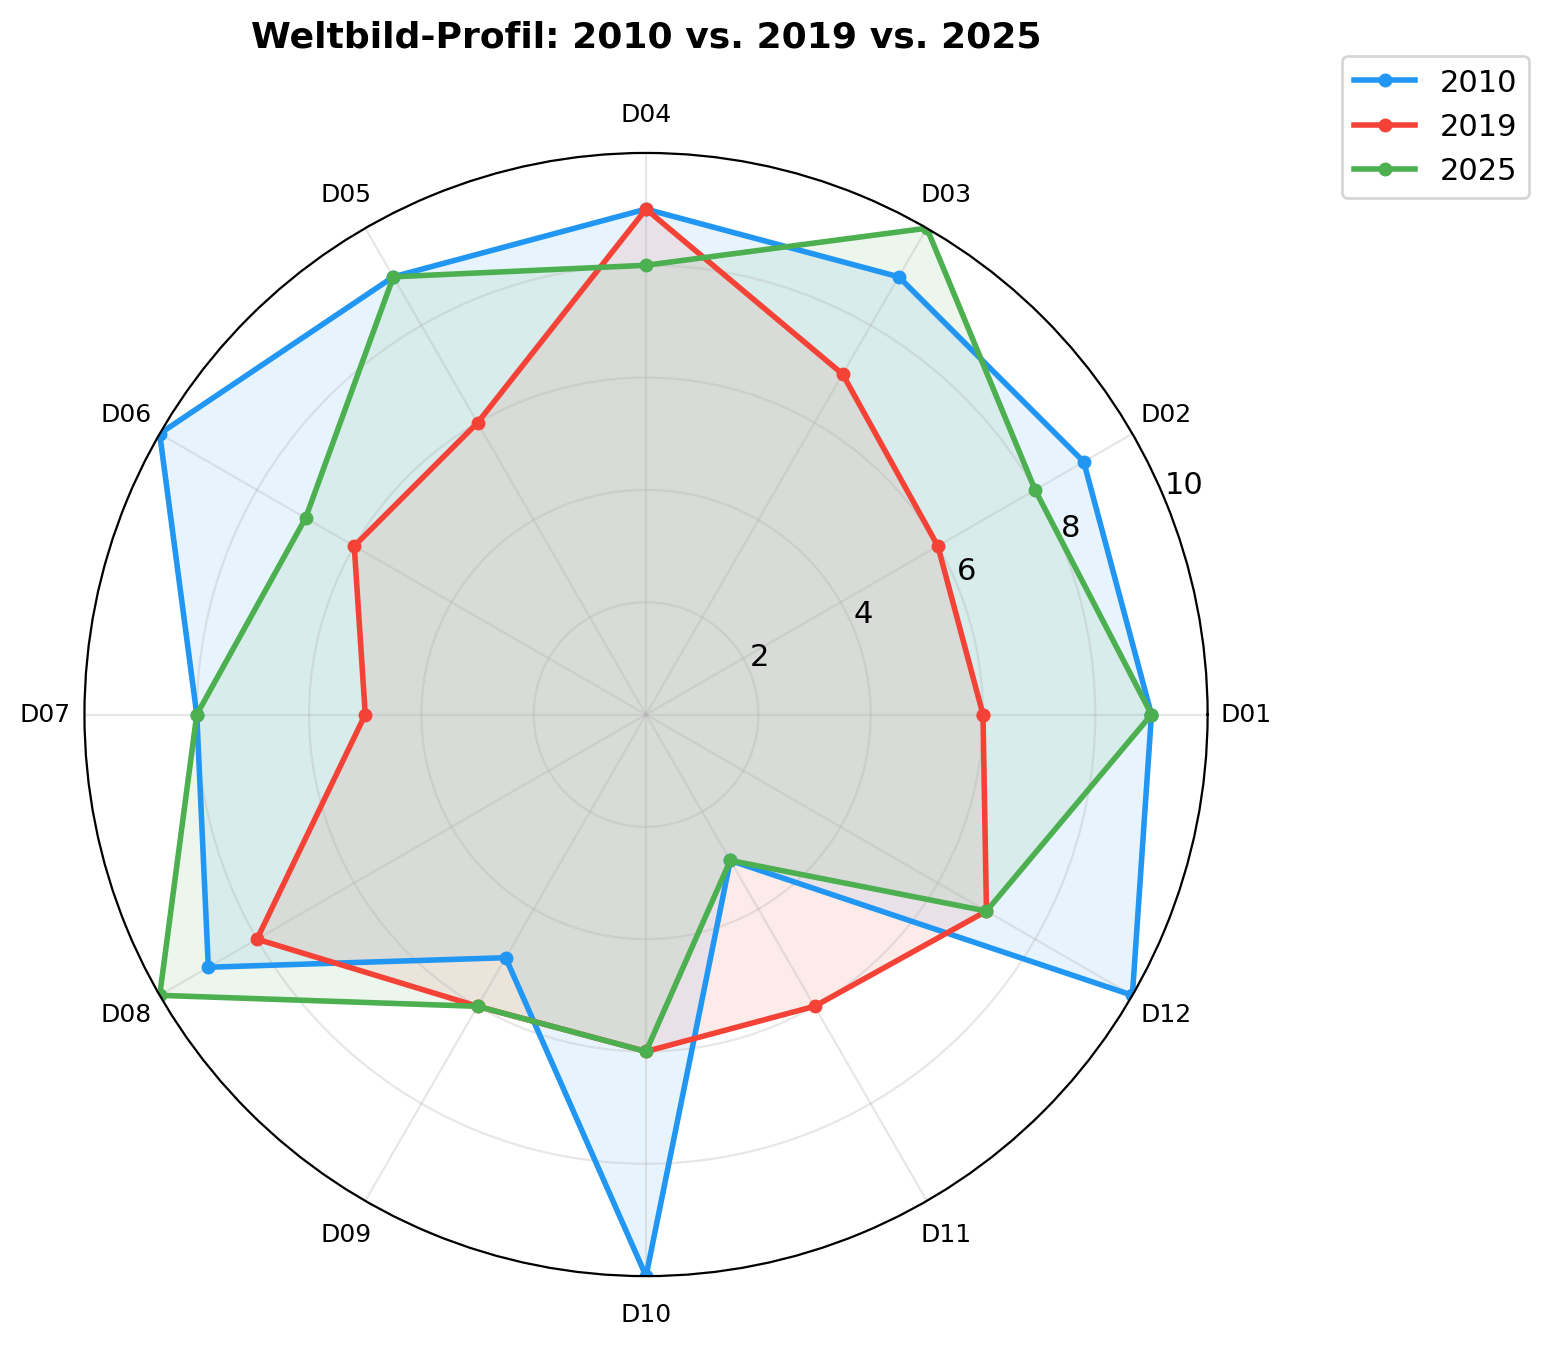
\includegraphics[width=0.85\textwidth]{fig3_radar_vergleich.png}
  \caption{Radar-Diagramm der vier Weltbild-Typen auf den 12 Dimensionen. Die Polarisierung zwischen Architekt (außen) und Hüter (innen) sowie die distinkte Position des Befreiers (hoher Egalitarismus bei niedriger Machtkonzentration) sind sichtbar.}
  \label{fig:radar}
\end{figure}

\medskip
\noindent\textbf{Kernbefund F4:} Die stärkste Polarisierung besteht zwischen Typ~I (Herrschaftslogik) und Typ~II (Teilhabelogik). Die explorative Vier-Cluster-Lösung bedarf einer konfirmatorischen Validierung an unabhängigen Daten, bevor sie als robustes Ergebnis gelten kann.


\subsubsection{Algorithmische Validierung der Clusterstruktur}

Um zu prüfen, ob die vier Weltbild-Typen natürlichen Daten-Clustern entsprechen, wurde HDBSCAN (dichtebasiertes Clustering) und KMeans auf die $100 \times 12$-Ratingmatrix angewendet. \textbf{HDBSCAN auf dem vollen 12-dimensionalen Raum} klassifiziert 80--100\,\% der Fälle als Rauschen über alle getesteten Parameterkonfigurationen (\texttt{min\_cluster\_size} $\in \{5, 8, 10, 15\}$, \texttt{min\_samples} $\in \{3, 5\}$); die beste Lösung findet nur 2~Cluster mit einem negativen Silhouette-Score ($-0{,}15$). KMeans mit $k = 4$ liefert einen Silhouette-Score von lediglich 0,169 -- deutlich unter dem Schwellenwert von 0,25, der typischerweise als Hinweis auf bedeutsame Struktur gilt.

\textbf{Subspace-Clustering} zeigt jedoch ein differenziertes Bild. Auf den beiden stärksten diskriminierenden Dimensionen (D07~Machtkonzentration und D11~Egalitarismus) identifiziert HDBSCAN mit \texttt{min\_cluster\_size}$\,=5$, \texttt{min\_samples}$\,=2$ neun Cluster mit einem \emph{Silhouette}-Score von \textbf{0,57} (12\,\% Rauschen) -- ein Hinweis auf substanzielle lokale Struktur in genau jenen Dimensionen, die die vier Idealtypen trennen. Analoges Subspace-Clustering auf den drei höchstladenden PCA-Dimensionen (D02, D05, D09) ergibt einen Silhouette-Score von 0,55. Zu beachten ist allerdings eine Zirkularitätsproblematik: D07 und D11 sind genau jene Dimensionen, die die Architekt-Befreier-Achse in der heuristischen Typologie definieren. Das Subspace-Clustering reproduziert dadurch teilweise das Auswahlkriterium, anstatt eine unabhängige Validierung zu liefern. Damit wird zwar die dimensionale Separabilität bestätigt, nicht aber die Unabhängigkeit der Validierung von der Typologie-Konstruktion.

Dieses Muster bestätigt den epistemologischen Status der vier Typen: Es handelt sich um \textbf{Webersche Idealtypen} -- heuristische Verdichtungen eines mehrdimensionalen Kontinuums, nicht um emergente Daten-Cluster. Ihr analytischer Nutzen wird durch diesen Befund nicht geschmälert; im Gegenteil, er wird durch hochsignifikante Kruskal--Wallis-Ergebnisse über die vier Typen bestätigt (Tabelle~\ref{tab:kruskal}).

\begin{table}[htbp]
  \centering
  \caption{Kruskal--Wallis-$H$-Test über die vier Weltbild-Typen ($df = 3$, $N = 100$). Signifikanz: {*}{*}{*}\,$p < 0{,}001$, {*}\,$p < 0{,}05$, n.s.\,=\,nicht signifikant. \textsuperscript{a}Nicht signifikant nach Bonferroni-Korrektur ($\alpha_{\mathrm{adj}} = 0{,}004$). Hinweis: Diese Tests beschreiben Muster innerhalb LLM-generierter Rekonstruktionen; $p$-Werte sind nominal und sollten nicht als inferenzstatistische Hypothesentests im klassischen Sinne interpretiert werden.}
  \label{tab:kruskal}
  \footnotesize
  \begin{tabular}{l c c l}
    \toprule
    \textbf{Dimension} & $H$ & $p$ & \textbf{Sig.} \\
    \midrule
    D02 Selbstwirksamkeit & 33,55 & $< 0{,}001$ & {*}{*}{*} \\
    D06 Fortschrittsglaube & 29,55 & $< 0{,}001$ & {*}{*}{*} \\
    D07 Machtkonzentration & 64,76 & $< 0{,}001$ & {*}{*}{*} \\
    D09 Menschenfreundlichkeit & 17,50 & $< 0{,}001$ & {*}{*}{*} \\
    D11 Egalitarismus & 49,57 & $< 0{,}001$ & {*}{*}{*} \\
    D12 Kontrollüberzeugung & 17,93 & $< 0{,}001$ & {*}{*}{*} \\
    \midrule
    D04 Verantwortungsgefühl & 10,76 & 0,013 & {*}\textsuperscript{a} \\
    D05 Techno-Determinismus & 11,21 & 0,011 & {*}\textsuperscript{a} \\
    \midrule
    D01 Sendungsbewusstsein & 2,59 & 0,459 & n.s. \\
    D03 Arbeitsethos & 3,75 & 0,290 & n.s. \\
    D08 Dringlichkeit & 6,25 & 0,100 & n.s. \\
    D10 Posthumanismus & 4,04 & 0,257 & n.s. \\
    \bottomrule
  \end{tabular}
\end{table}

Nach Bonferroni-Korrektur für 12 simultane Tests ($\alpha_{\mathrm{adj}} = 0{,}05/12 = 0{,}004$) erreichen D04 ($p = 0{,}013$) und D05 ($p = 0{,}011$) nicht mehr Signifikanz. Die sechs Dimensionen mit $p < 0{,}001$ bleiben nach Korrektur signifikant. Sechs von zwölf Dimensionen zeigen somit hochsignifikante Inter-Typ-Unterschiede ($p < 0{,}001$), während zwei weitere Dimensionen (D04, D05) nominale Signifikanz auf dem $p < 0{,}05$-Niveau erreichen, aber die Bonferroni-Korrektur nicht überstehen. Die vier nicht-signifikanten Dimensionen (D01, D03, D08, D10) repräsentieren den \emph{geteilten Kern} des KI-Elite-Weltbilds -- Überzeugungen, bei denen alle vier Typen konvergieren. D07 (Machtkonzentration, $H = 64{,}76$) und D11 (Egalitarismus, $H = 49{,}57$) sind die diskriminierendsten Dimensionen. Ein Zirkularitätsvorbehalt gilt: Da die vier Typen teilweise \emph{durch} D07 und D11 definiert wurden, spiegeln die hohen $H$-Werte auf diesen Dimensionen teilweise das Konstruktionskriterium wider, nicht eine unabhängige Validierung. Die Kruskal--Wallis-Ergebnisse für die übrigen Dimensionen (D02, D06, D09, D12) sind informativer, da sie nicht in die Typenkonstruktion eingingen.


\subsection{F5 -- Subgruppenvergleiche}
\label{sec:ergebnisse:f5}

Die Inter-Gruppen-Vergleiche bilden den analytischen Kern der Studie. Durch den systematischen Vergleich der kollektiven Weltbilder soziologisch definierter Gruppen -- differenziert nach institutioneller Rolle, ideologischer Haltung, Geschlecht, Firmenzugehörigkeit und Regulierungsposition -- deckt die Analyse auf, welche strukturellen Faktoren die kollektiven Überzeugungen innerhalb der KI-Elite am stärksten prägen. Tabelle~\ref{tab:subgruppen} ordnet die sechs diskriminierendsten Vergleiche.

\begin{table}[htbp]
  \centering
  \caption{Ranking der Subgruppen-Differenzen. $\Delta$ = Gr.~1 $-$ Gr.~2 (Durchschnitt); Einzelkontraste beziehen sich auf die Dimension mit der größten Abweichung.}
  \label{tab:subgruppen}
  \small
  \begin{tabular}{c l c c c l}
    \toprule
    \textbf{Rang} & \textbf{Vergleich} & \textbf{Avg Gr.~1} & \textbf{Avg Gr.~2} & $\Delta$ & \textbf{Stärkster Kontrast} \\
    \midrule
    1 & Risiko vs.\ Speed   & 5,9 & 7,6 & 1,7 & D02, D06, D10, D12: je $-5$ \\
    \addlinespace[2pt]
    2 & CEOs vs.\ Akademiker & 7,8 & 6,3 & 1,5 & D07: $+4$, D11: $-4$ \\
    \addlinespace[2pt]
    3 & Frauen vs.\ Männer & 6,9 & 8,1 & 1,2 & D11: $-6$ \\
    \addlinespace[2pt]
    4 & Open vs.\ Closed     & 6,8 & 6,3 & 0,5 & D07: $-3$, D12: $+3$ \\
    \addlinespace[2pt]
    5 & Reg-Pro vs.\ Contra  & 6,3 & 6,8 & 0,5 & D04: $+4$, D06: $-3$ \\
    \addlinespace[2pt]
    6 & Anthropic vs.\ OpenAI & 6,9 & 7,3 & 0,4 & D12: $-3$ \\
    \bottomrule
  \end{tabular}
\end{table}

\begin{figure}[htbp]
  \centering
  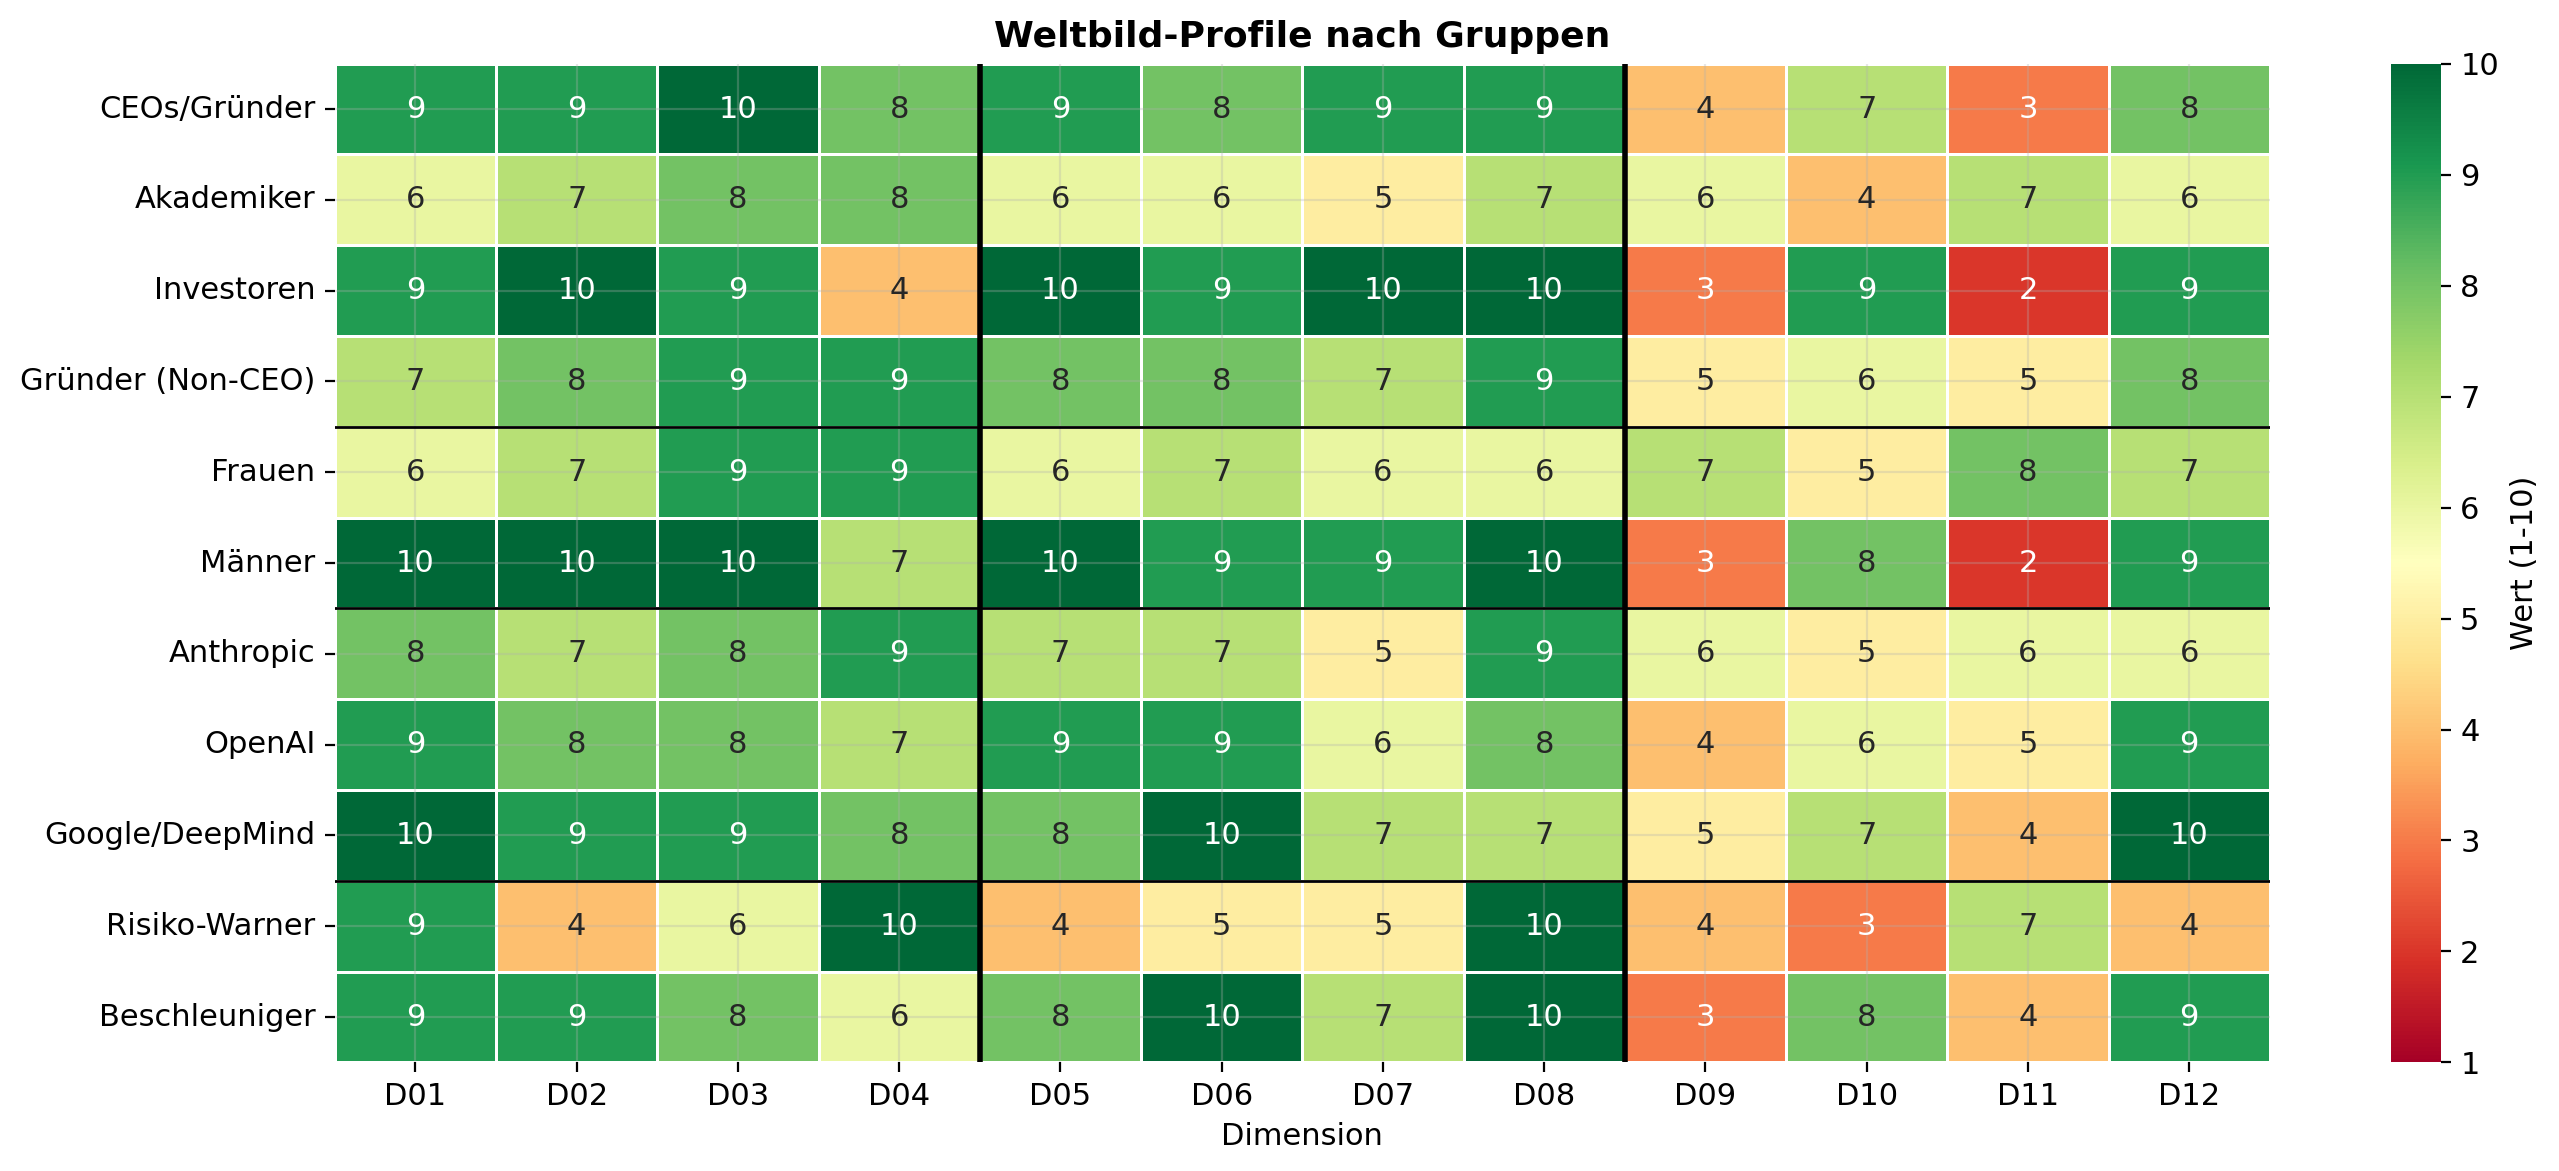
\includegraphics[width=\textwidth]{fig5_gruppen_heatmap.png}
  \caption{Gruppen-Heatmap: 15 Subgruppen $\times$ 12 Dimensionen. Die systematische Variation von D07 (Machtkonzentration) und D11 (Egalitarismus) über alle Vergleiche hinweg ist der zentrale visuelle Befund.}
  \label{fig:gruppen_heatmap}
\end{figure}

Der \textbf{stärkste Kontrast} (Risiko vs.\ Speed, $\Delta$~1,7) betrifft nicht die Risikoeinschätzung -- beide Seiten veranschlagen die Katastrophenwahrscheinlichkeit auf 10--20\,\% --, sondern die ontologische Vorfestlegung: Risiko-Warner konzipieren KI als potenziellen autonomen Agenten, Beschleuniger als Werkzeug.

\textbf{Effektstärken (Cliff's $\delta$)} quantifizieren diese Kontraste nicht-parametrisch (Schwellenwerte nach \citealt{Romano2006}: $|\delta| < 0{,}147$ vernachlässigbar, $0{,}147$--$0{,}33$ klein, $0{,}33$--$0{,}474$ mittel, $> 0{,}474$ groß). Die extremsten paarweisen Unterschiede zwischen den vier Weltbild-Typen treten auf der Macht-Egalitarismus-Achse auf: Architekt vs.\ Befreier ergibt $\delta = +1{,}0$ auf D07 (Machtkonzentration) und $\delta = -0{,}98$ auf D11 (Egalitarismus) -- effektiv perfekte Separation. Architekt vs.\ Hüter erreicht $\delta = +1{,}0$ auf D07 und $\delta = -0{,}68$ auf D11. Über alle sechs Cluster-Paare hinweg produzieren D07 und D11 jeweils fünf mittlere bis große Effekte ($|\delta| \geq 0{,}33$), was sie als primäre Diskriminierungsdimensionen bestätigt.

\textbf{Rollenbasierte Vergleiche} zeigen ähnlich starke Effekte: Akademiker vs.\ Investoren unterscheiden sich auf 9 von 12~Dimensionen mit \emph{großem} Effekt (am deutlichsten D02~Selbstwirksamkeit: $\delta = -0{,}88$; D12~Kontrollüberzeugung: $\delta = -0{,}71$; D09~Menschenfreundlichkeit: $\delta = +0{,}68$). CEOs vs.\ Akademiker zeigen große Effekte auf 6~Dimensionen (D02: $\delta = +0{,}79$; D06: $\delta = +0{,}58$; D12: $\delta = +0{,}55$).

\textbf{Gender-Unterschiede} erreichen Signifikanz auf 7 von 12~Dimensionen. Die größten Effekte betreffen D09~Menschenfreundlichkeit ($\delta = +0{,}59$, groß: Frauen höher), D05~Techno-Determinismus ($\delta = -0{,}50$, groß: Männer höher) und D11~Egalitarismus ($\delta = +0{,}46$, mittel). Diese Effektstärken sind moderater als die nominalen Gruppenkontraste ($\Delta = 6$) vermuten ließen, was zu erwarten ist: Cliff's $\delta$ erfasst die volle Verteilungsüberlappung, nicht nur Mittelwerte. Der oben genannte Kontaminationsvorbehalt gilt in vollem Umfang.

Tabelle~\ref{tab:effektstaerken} fasst diese nicht-parametrischen Effektstärken über die vier Weltbild-Typen, institutionelle Rollen und Geschlecht zusammen.

\begin{table}[htbp]
  \centering
  \caption{Nicht-parametrische Effektstärken (Cliff's $\delta$) für zentrale Paarvergleiche nach Typen, Rollen und Geschlecht. Schwellenwerte nach \citet{Romano2006}: $|\delta| < 0{,}147$ vernachlässigbar, $0{,}147$--$0{,}33$ klein, $0{,}33$--$0{,}474$ mittel, $> 0{,}474$ groß.}
  \label{tab:effektstaerken}
  \small
  \resizebox{\textwidth}{!}{%
  \begin{tabular}{l l c l c}
    \toprule
    \textbf{Vergleichsbereich} & \textbf{Paarweiser Vergleich} & \textbf{Schlüsseldim.} & \textbf{Dimensionsname} & \textbf{Cliff's $\delta$} \\
    \midrule
    Weltbild-Typen & Architekt vs.\ Befreier & D07 & Machtkonzentration   & $+1{,}00$ (groß) \\
                   &                         & D11 & Egalitarismus        & $-0{,}98$ (groß) \\
                   \addlinespace[2pt]
                   & Architekt vs.\ Hüter    & D07 & Machtkonzentration   & $+1{,}00$ (groß) \\
                   &                         & D11 & Egalitarismus        & $-0{,}68$ (groß) \\
    \midrule
    Institutionelle Rollen & Akademiker vs.\ Investoren & D02 & Selbstwirksamkeit     & $-0{,}88$ (groß) \\
                           &                            & D12 & Kontrollüberzeugung   & $-0{,}71$ (groß) \\
                           &                            & D09 & Menschenfreundlichkeit& $+0{,}68$ (groß) \\
                           \addlinespace[2pt]
                           & CEOs vs.\ Akademiker       & D02 & Selbstwirksamkeit     & $+0{,}79$ (groß) \\
                           &                            & D06 & Fortschrittsglaube    & $+0{,}58$ (groß) \\
                           &                            & D12 & Kontrollüberzeugung   & $+0{,}55$ (groß) \\
    \midrule
    Geschlechterdifferenzen & Frauen vs.\ Männer         & D09 & Menschenfreundlichkeit& $+0{,}59$ (groß) \\
                            &                            & D05 & Techno-Determinismus  & $-0{,}50$ (groß) \\
                            &                            & D11 & Egalitarismus        & $+0{,}46$ (mittel) \\
    \bottomrule
  \end{tabular}%
  }
\end{table}

Der \textbf{größte nominale Einzelkontrast} der gesamten Erhebung findet sich bei D11 im Gender-Vergleich: sechs volle Skalenpunkte (Frauen:~8, Männer:~2). Das Frauen-Weltbild ist kein Anti-Technik-Weltbild, sondern ein \emph{konditioniertes} Technik-Weltbild: gleich optimistisch, aber mit stärkeren ethischen Bedingungen. Dieser Befund ist jedoch der \emph{am stärksten kontaminationsgefährdete} der gesamten Studie und wird daher als \emph{vorläufige Hypothese} eingestuft, nicht als gesicherter Befund. Die Gründe: (a)~LLMs reproduzieren bekannte Gender-Stereotypen, insbesondere die Zuschreibung erhöhter sozialer Orientierung an Frauen~\citep{Santurkar2023}; (b)~die Frauenstichprobe ist klein ($n = 18$); (c)~die Effektgröße ($\Delta = 6$) übersteigt das in vergleichbaren empirischen Studien beobachtete Ausmaß deutlich. Eine unabhängige Validierung -- idealerweise durch Replikation anderer Forschungsteams mit verschiedenen Modellen und Expertenratings -- ist für diesen Befund besonders dringlich.

Die \textbf{größte Überraschung} liegt im Regulierungsvergleich: Anti-Regulierer haben den niedrigsten Machtkonzentrations-Wert aller 15~Gruppen (D07=2). Dies widerlegt das verbreitete Narrativ, Anti-Regulierer seien Vertreter von Konzerninteressen.

\medskip
\noindent\textbf{Kernbefund F5:} Die drei stärksten Prädiktoren für das Weltbild sind die ideologische Grundhaltung, die institutionelle Rolle und das Geschlecht. Die polarisierendsten Dimensionen sind D11 und D07. Die \emph{Machtfrage} ist der Kern der internen Differenzen.


\subsection{F6 -- Macht und Weltbild}
\label{sec:ergebnisse:f6}

\emph{Macht} wird in dieser Studie operativ als Ressourcenkontrolle verstanden: die Fähigkeit, über Kapital, Compute-Infrastruktur, Forschungsteams und politischen Zugang zu verfügen und dadurch die Richtung der KI-Entwicklung zu beeinflussen. Diese Definition folgt dem soziologischen Machtbegriff im Sinne Webers (\glqq Chance, den eigenen Willen auch gegen Widerstreben durchzusetzen\grqq) und Bourdieus (Kapitalakkumulation als Machtmechanismus), ohne eine umfassende machttheoretische Analyse zu beanspruchen.

\begin{table}[htbp]
  \centering
  \caption{Weltbild-Typen und Ressourcen-Kontrolle.}
  \label{tab:macht}
  \begin{tabular}{l c c c l}
    \toprule
    \textbf{Typ} & \textbf{Avg} & \textbf{D11} & \textbf{D04} & \textbf{Ressourcen} \\
    \midrule
    I Architekt  & 7,8 & 2,8 & 6,3 & Höchste \\
    \addlinespace[2pt]
    III Innovator & 7,2 & 5,0 & 8,3 & Hoch \\
    \addlinespace[2pt]
    IV Befreier  & 6,8 & 7,5 & 6,0 & Mittel \\
    \addlinespace[2pt]
    II Hüter   & 6,4 & 7,2 & 9,0 & Geringste \\
    \bottomrule
  \end{tabular}
\end{table}

Die Daten aus F4 (Cluster-Analyse) weiterverfölgend, zeigt sich ein zusätzliches Muster auf der Machtebene: Je höher die Weltbild-Intensität, desto niedriger die Werte bei Menschenfreundlichkeit und Egalitarismus und desto höher die Machtkonzentrations-Akzeptanz. Das Investoren-Profil markiert den Extremfall: maximale Kontrollüberzeugung (D02=10) bei minimalem Verantwortungsgefühl (D04=4) -- \glqq Macht ohne Rechenschaft\grqq. Das bereits in F1 beobachtete Muster (vgl.\ Abschnitt~\ref{sec:ergebnisse:f1}) verschärft sich: Macht intensiviert alle Überzeugungen -- ausgenommen jene, die Macht selbst in Frage stellen.

\medskip
\noindent\textbf{Kernbefund F6:} Die rekonstruierten Profile zeigen ein auffälliges Muster: Gruppen mit höherer Ressourcenkontrolle weisen intensivere Weltbild-Werte auf, bei gleichzeitig niedrigeren Werten bei Egalitarismus und Verantwortung. Da beide Seiten dieser Beobachtung auf LLM-Rekonstruktionen basieren, ist unklar, ob die Korrelation empirische Realität oder interne Modellkohärenz widerspiegelt. Falls robust, wäre dies der demokratietheoretisch relevanteste Befund der Studie.


%% =============================================================================
%% ZUSAMMENFASSUNG DER KERNBEFUNDE
%% =============================================================================

\begin{table}[htbp]
  \centering
  \caption{Synopse der sechs Kernbefunde: Ergebnis, Konfidenz, Validierungsstatus und epistemischer Status. Konfidenz-Einstufung: \emph{Hoch} = stabil über $\geq 3$ Gruppen-Synthesen und durch Inter-Gruppen-Konsistenz oder interne Kohärenzprüfung gestützt; \emph{Mittel-hoch} = stabil, aber ohne externe Validierung; \emph{Mittel} = explorativ, abhängig von Cluster-Lösung oder kleiner Subgruppe. Epistemischer Status: (D)~=~deskriptiv, (E)~=~explorativ, (H)~=~hypothesengenerierend.}
  \label{tab:synopse}
  \footnotesize
  \begin{tabularx}{\textwidth}{l Y c c c}
    \toprule
    \textbf{F} & \textbf{Kernbefund} & \textbf{Konfidenz} & \textbf{Extern val.?} & \textbf{Status} \\
    \midrule
    F1 & Technologischer Messianismus mit Ambivalenzstruktur (Avg~7,1; Doppelsenke D09/D11) & Hoch & Inter-Gruppen & (D) \\
    \addlinespace[3pt]
    F2 & Utopie-Komplex erodiert; tragischer Beschleunigungszwang (D10: $-2{,}4$/Dek.) & Mittel-hoch & Nein & (D) \\
    \addlinespace[3pt]
    F3 & Richtungsabhängige Sagen-Handeln-Kluft (D07 $+2$, D11 $-2$; stabil über v1/v2) & Mittel & Nein & (H) \\
    \addlinespace[3pt]
    F4 & Vier Weltbild-Typen: Architekt, Hüter, Innovator, Befreier & Mittel & Nein & (E) \\
    \addlinespace[3pt]
    F5 & Stärkste Prädiktoren: Haltung, Rolle, Gender (vorläufig) & Mittel & Nein & (E) \\
    \addlinespace[3pt]
    F6 & Macht-Gemäßigtheits-Paradox: Macht $\sim$ Extremität & Hoch & Nein & (H) \\
    \bottomrule
  \end{tabularx}
\end{table}


%% =============================================================================
%% 5. DISKUSSION
%% =============================================================================
\section{Diskussion}
\label{sec:diskussion}

\subsection{Zusammenfassung und Interpretation}
\label{sec:diskussion:zusammenfassung}

Die Ergebnisse \emph{legen nahe}, dass die KI-Elite, auf Gruppenebene analysiert, ein Muster aufweist, das sich idealtypisch als \emph{technologischer Messianismus mit struktureller Ambivalenz} beschreiben lässt. Die Metapher des \glqq Messianismus\grqq{} ist dabei analytisch gemeint -- als Bezeichnung für die Kombination aus hohem Sendungsbewusstsein, Techno-Determinismus und Dringlichkeit --, nicht als Werturteil oder psychologisierende Zuschreibung. Der Begriff grenzt sich von verwandten Konzepten ab: \citeauthor{Morozov2013}s \glqq Solutionismus\grqq{} erfasst die Problemlösungshaltung, nicht die quasi-religiöse Dringlichkeit; \glqq Techno-Utopismus\grqq{} impliziert positiven Zukunftsglauben, der laut F2 gerade erodiert; \glqq technologischer Messianismus\grqq{} bezeichnet spezifisch die Persistenz eines erlöserischen Handlungsimperativs \emph{trotz} schwindendem Zukunftsoptimismus. Die sechs Forschungsfragen fügen sich zu einem in sich stimmigen Bild: F1~weist auf die \glqq Doppelsenke\grqq{} bei D09 und D11 als kollektives Merkmal hin; F2~deutet auf eine Erosion des Utopie-Komplexes über die Epochen hin; F3~zeigt richtungsabhängige Sagen-Handeln-Diskrepanzen auf spezifischen Dimensionen (D07, D11), wobei die Gesamtmagnitude der Kluft vorsichtiger Interpretation bedarf; F4~differenziert vier Weltbild-Typen mit antagonistischen kollektiven Positionen; F5 und F6 vervollständigen das Bild durch das Macht-Gemäßigtheits-Paradox. Die Inter-Gruppen-Vergleiche (F5) bilden das analytische Herz der Studie: Der Befund, dass institutionelle Rolle, ideologische Haltung und Geschlecht die kollektiven Überzeugungsstrukturen systematisch formen, trägt direkte Implikationen für KI-Governance und demokratische Theorie. Alle Befunde basieren auf LLM-generierten Rekonstruktionen auf Gruppenebene und sind daher als \emph{empirisch gestützte Hypothesen} zu verstehen, nicht als bewiesene Tatsachen. Formulierungen wie \glqq zeigt\grqq{} und \glqq offenbart\grqq{} sind durchgängig im Sinne von \glqq die Daten legen nahe\grqq{} zu lesen.

Überraschend ist erstens die Richtungskonsistenz der Sagen-Handeln-Diskrepanzen über Messbedingungen hinweg (D07/D11 stabil in v1 und v2); zweitens der Rückzug des Posthumanismus (D10 von 10 auf 6 -- widerlegt die gängige Annahme zunehmend posthumanistischer Orientierung); drittens die Existenz des Befreier-Typs (Opposition gegen Machtkonzentration auch von libertärer Seite); viertens die Konsistenz der Muster auf Gruppenebene über mehrere unabhängige Synthesen hinweg.


\subsection{Einordnung in den Forschungsstand}
\label{sec:diskussion:einordnung}

\citeauthor{Morozov2013}s Solutionismus-These findet eine nahezu vollständige Bestätigung (D05=8--9, D06=7--9). Allerdings ist der Solutionismus kein monolithischer Block: Risiko-Warner (D05=4) teilen ihn deutlich weniger. Er ist die Ideologie des mächtigsten Segments, nicht der KI-Elite schlechthin.

\citeauthor{Daub2020}s Analyse der philosophischen Tiefenstrukturen wird durch die narrativen Synthesen bestätigt. Was die vorliegende Studie hinzufügt, ist die \emph{Quantifizierung} und die Demonstration, dass sich die Intensität systematisch mit der Machtposition verstärkt.

Die von~\citet{BarbCam1996} diagnostizierte Californian Ideology findet in der Existenz des Befreier-Typs ihre zeitgenössische Entsprechung -- empirisch nachweisbar dreißig Jahre später.

\citeauthor{Coeckelbergh2020}s Annahme einer zunehmenden Enhancement-Orientierung wird durch die rekonstruierten Trends partiell \emph{in Frage gestellt}: Der deutliche Rückgang des Posthumanismus (D10 von 10 auf 6) legt nahe, dass das Interesse der KI-Elite an der technologischen Transformation des Menschen selbst abgenommen hat -- zugunsten einer Fokussierung auf autonome KI-Systeme als eigenständige Akteure. Dabei sind drei alternative Erklärungen in Betracht zu ziehen: (a)~der Rückgang könnte ein \emph{Diskursartefakt} sein -- posthumanistische Themen sind nach 2020 medial weniger präsent, was die Datendichte entsprechender Aussagen reduziert; (b)~die Position könnte nicht verschwunden, sondern in neue Begriffe transformiert worden sein (\glqq AGI\grqq{} statt \glqq Enhancement\grqq); (c)~der Trend könnte eine strategische \emph{Selbstzensur} reflektieren, da posthumanistische Rhetorik politisch toxischer geworden ist.

\emph{Zum Gender-Befund.} Der in F5 berichtete extreme Kontrast bei D11 (Frauen:~8, Männer:~2, $\Delta = 6$) ist der größte Einzelkontrast der gesamten Erhebung, aber zugleich der am stärksten kontaminationsgefährdete. LLMs reproduzieren bekannte Gender-Stereotypen -- insbesondere die Zuschreibung erhöhter Empathie und sozialer Orientierung an Frauen~\citep{Santurkar2023}. Da die Frauenstichprobe klein ist ($n = 18$) und die Ratings vom selben LLM generiert wurden, das diese Stereotypen internalisiert hat, ist nicht unterscheidbar, ob der Kontrast (a)~eine reale Differenz in den Weltbildern, (b)~ein LLM-Stereotyp-Artefakt oder (c)~eine Mischung aus beidem reflektiert. Der Befund wird daher als \emph{Hypothese} berichtet, die einer unabhängigen Validierung -- idealerweise durch Replikation anderer Forschungsteams mit verschiedenen Instrumenten und Expertenratings -- bedarf.

Die von~\citet{TorresGebru2024} vorgeschlagene TESCREAL-Taxonomie (Transhumanism, Extropianism, Singularitarianism, Cosmism, Rationalism, Effective Altruism, Longtermism) findet in der Vier-Cluster-Lösung eine empirische Ausdifferenzierung: Der Architekt-Typ verkörpert die machtpolitische Seite des TESCREAL-Bündels (Singularitarianism, Longtermism), der Hüter-Typ dessen institutionelle Kritik (Effective Altruism mit Sicherheitsfokus), der Befreier-Typ den libertären Extropianismus. Was die TESCREAL-Analyse als monolithisches Ideologiebündel beschreibt, zeigt sich in den Daten als Spektrum mit mindestens vier distinkten Positionen. \citet{Becker2025} ergänzt diese Perspektive durch die Analyse der \glqq Broligarchie\grqq{} als soziales Phänomen: Die Verschmelzung von technologischer Vision und männlicher Machtelite, die in der Gender-Analyse (F5, D11-Kontrast von 6~Skalenpunkten) ihren empirischen Niederschlag findet.

Paul Ricoeurs \glqq Hermeneutik des Verdachts\grqq{}~\citep{Ricoeur1970} bietet einen ergänzenden analytischen Rahmen: Hinter der scheinbar neutralen, technisch-rationalen Sprachoberfläche der KI-Eliten-Kommunikation verbergen sich Machtinteressen und Klassendynamiken, die erst durch systematische Dekonstruktion sichtbar werden. Die SWR-Kongruenzanalyse (F3) operationalisiert diesen Verdacht empirisch: Die $\Delta$-Werte zwischen Sagen und Handeln zeigen präzise, \emph{wo} die performative Oberfläche von der operativen Realität abweicht.

Aus wissenschaftssoziologischer Perspektive lässt sich der Rückgang des Egalitarismus (D11) als Erosion der Merton'schen Wissenschaftsnormen lesen~\citep{Merton1973}: Communalism (offener Zugang), Universalism und Organized Skepticism weichen zunehmend proprietären, beschleunigungszentrierten Logiken. Der Übergang von Forschungspublikation zu Produkt-Launch als primärem Output-Format ist ein sichtbarer Marker dieser Verschiebung.

Die Vier-Cluster-Lösung lässt sich darüber hinaus feldtheoretisch lesen: Die antagonistische Struktur zwischen Architekt (ökonomisches Kapital) und Hüter (symbolisches Kapital) reproduziert das von~\citet{Bourdieu1992} für das intellektuelle und künstlerische Feld diagnostizierte Muster einer \emph{umgekehrten ökonomischen Welt}. Im KI-Feld gilt: Wer die meisten Ressourcen kontrolliert, hat die geringste Legitimation durch Gemeinwohlorientierung -- und umgekehrt. Das Macht-Gemäßigtheits-Paradox (F6) lässt sich in dieser Perspektive als strukturelle Eigenschaft des Feldes lesen -- wobei die explorative Natur der Cluster-Daten keine konfirmatorische Aussage erlaubt.

Das Forschungsupdate 2026 ergänzt vier direkt einschlägige Randbedingungen. Tabelle~\ref{tab:research_update_ledger} führt keine neuen Ratings ein und ersetzt keine berichteten empirischen Outputs; sie macht sichtbar, wie die neue Literatur gegen die bestehenden SWR-Oberflächen gelesen werden sollte und wo die Claim-Grenze liegt.

\begin{table}[htbp]
  \centering
  \caption{Forschungsupdate-Ledger 2026 für Paper A.}
  \label{tab:research_update_ledger}
  \scriptsize
  \begin{tabularx}{\textwidth}{@{} L{3.0cm} L{2.8cm} L{3.4cm} Y @{}}
    \toprule
    \textbf{Quellensignal 2026} & \textbf{SWR-Anker} & \textbf{Präsentationsgewinn} & \textbf{Claim-Grenze} \\
    \midrule
    Techno-Supremacy-Doktrin im Diskurs der KI-Führungselite \citep{PerezUrbina2026TechnoSupremacy} & D01/D05/D08/D10; Architekt-Innovator-Kontrast & Externer KDA-Abgleich für Messianismus, Unvermeidbarkeit und Risiko-als-Techniklösung-Muster & Stützt nur Diskursanschluss; beweist nicht, dass alle Subgruppen eine einheitliche Doktrin teilen. \\[3pt]
    Big-AI-Regulatory-Capture-Taxonomie \citep{BirhaneEtAl2026RegulatoryCapture} & D07/D11; F6; Sagen-Handeln-Dimensionen & Übersetzt die Macht-Gleichheits-Achse in prüfbare Regulatory-Capture-Mechanismen für ein künftiges v9-Ledger & Mechanismuskandidat, keine Absichts- oder Kausalbehauptung über Akteure. \\[3pt]
    Infrastruktur-Souveränitätsgrenze \citep{Cruzes2026InfrastructureSovereignty} & D07 materielle Macht; D11 Zugang; Macht-Gemäßigtheits-Paradox & Erweitert die Ressourcenkontroll-Lesart von Diskurs und Regulierung auf Rechenkapazitäts-, Netz-, Energie- und Telemetrie-Engpassstellen & Nur Kontextschicht; dieser Datensatz misst Infrastruktur-Eigentum nicht direkt. \\[3pt]
    GenAI-Persona-Scoping-Review \citep{AminEtAl2026GenAIPersonas} & Methodik; Limitationen; Validierungsübersicht & Schärft die Trennung zwischen SWR-Rekonstruktion und GenAI-Persona- oder Survey-Ersatz & Stützt den Methodenvorbehalt; validiert die SWR-Ratings nicht extern. \\
    \bottomrule
  \end{tabularx}
\end{table}

Der spezifische Mehrwert gegenüber essayistischen Diagnosen liegt in drei Punkten: \emph{Masse} (100 Personen, 16 Jahre), \emph{Differenzierung} (vier distinkte Typen) und \emph{Validierung} (Kongruenzanalyse als empirischer Test).


\subsection{Agentic Alignment vs.\ Worldview Alignment}
\label{sec:diskussion:alignment}

Die in F3 angezeigten richtungsabhängigen Sagen-Handeln-Diskrepanzen (am robustesten: D07 Machtkonzentration $\Delta = +2$, D11 Egalitarismus $\Delta = -2$, stabil über Messbedingungen) lassen sich mit einer in dieser Studie eingeführten begrifflichen Unterscheidung schärfer fassen, die auf Terminologie der KI-Alignment-Debatte zurückgreift.\footnote{Weder \emph{Worldview Alignment} noch \emph{Agentic Alignment} entsprechen in der hier verwendeten Bedeutung einem fest etablierten Begriff der KI-Alignment-Literatur; das Begriffspaar wird als analytische Heuristik für diese Studie eingeführt, um die performative von der operativen Ebene des Wertausdrucks zu unterscheiden.} \emph{Worldview Alignment} bezeichnet die rhetorische Reproduktion erwünschter Werte -- das öffentliche Bekenntnis zu Gleichheit, Verantwortung und Menschlichkeit, wie es die \glqq Sagen\grqq-Seite der Analyse erfasst. \emph{Agentic Alignment} bezeichnet die tatsächliche Ressourcenverteilung und Macht\-ausübung -- die \glqq Handeln\grqq-Seite. Die Befunde zeigen, dass die KI-Elite ein hohes Maß an Worldview Alignment aufweist (die \glqq richtigen\grqq{} Werte werden artikuliert), während das Agentic Alignment systematisch davon abweicht. Dieser Dualismus verbindet die vorliegende KI-Elite-Studie mit der breiteren Alignment-Debatte und wirft die Frage auf, ob die gegenwärtigen Bemühungen um \glqq AI Alignment\grqq{} nicht die performative Ebene (Worldview) mit der operativen (Agentic) verwechseln.


\subsection{Methodische Reflexion}
\label{sec:diskussion:methodik}

Die primäre Leistung der SWR liegt in der Verbindung qualitativer Tiefe mit quantitativer Systematik auf Gruppenebene. Die Studie identifiziert ein zuverlässiges Instrument -- Claude Opus~4.6, validiert durch Intra-Modell-Inter-Instanzen-Rating-Reliabilität (IMIIRR, ICC $= 0{,}902$) -- und demonstriert dessen konsistente Anwendung über alle Syntheseeinheiten. Dieser IMIIRR-Koeffizient übertrifft die typische Inter-Rater-Reliabilität menschlicher Kodierer in qualitativer Forschung (ICC $= 0{,}6$--$0{,}8$; \citealt{Hallgren2012}), und das Instrument bietet einen distinktiven Vorteil gegenüber menschlichen Kodierern: Vollständig dokumentierte Prompts ersetzen implizite Kodierregeln und ermöglichen exakte Replikation. Die Kongruenzanalyse (F3) fungiert als interner Validitätstest; die Stabilität des Kollektiv-Profils über 15~Gruppen-Synthesen und 4~Typen stärkt die Konvergenzvalidität. Die Inter-Gruppen-Vergleiche liefern eine eigene Form der Validierung: Wenn verschiedene Gruppensynthesen -- unabhängig voneinander aus unterschiedlichen Daten-Subsets produziert -- konsistente strukturelle Muster ergeben (z.\,B.\ die D07/D11-Achse als diskriminierendes Merkmal über alle Vergleiche hinweg), ist dies ein Beleg für die Robustheit der Methode, der über das hinausgeht, was eine einzelne Synthese leisten könnte. Die Replikation mit anderen Frontier-Modellen stellt eine unabhängige Forschungsaufgabe dar -- analog zur Replikation einer Befragung mit verschiedenen Interviewer-Teams -- und wird explizit als Desiderat für zukünftige Arbeiten identifiziert, nicht als Voraussetzung für die Validität der vorliegenden Studie. Die systematische Diskussion der methodischen Grenzen -- Kohärenzbias, Kontaminationsrisiko, Fokuskontrolllimits, Prompt-Sensitivität -- findet sich in Abschnitt~\ref{sec:limitationen}.


\subsection{Gesellschaftliche und politische Implikationen}
\label{sec:diskussion:implikationen}

Die Befunde auf Gruppenebene tragen direkte Implikationen für KI-Governance und demokratische Theorie. Das Macht-Gemäßigtheits-Paradox -- der systematische Befund, dass institutionelle Gruppen mit den meisten Ressourcen kollektive Weltbilder aufweisen, die am weitesten von demokratischen Idealen entfernt sind -- stellt eine konkrete Herausforderung für die Regulierungsarchitektur dar. Dieser Befund resoniert mit \citeauthor{Mills1956}' (\citeyear{Mills1956}) klassischer Analyse der \glqq Power Elite\grqq{} als sich selbst verstärkendes Stratum, dessen Weltbild systematisch von der breiteren Öffentlichkeit divergiert, und bestätigt die institutionenökonomische Analyse von~\citet{AcemogluJohnson2023}: Technologische Eliten tendieren dazu, Innovationen so zu lenken, dass sie bestehende Machtstrukturen verstärken, statt sie aufzubrechen -- ein Muster, das die Autoren historisch von der Industrialisierung bis zur Digitalisierung nachzeichnen. Gegenwärtige Governance-Ansätze (EU~AI~Act, Executive Order on AI) adressieren die technischen Artefakte, nicht die kollektiven Weltbilder der Gruppen, die diese Artefakte produzieren. Ein ergänzender Ansatz müsste die \emph{epistemische Diversität} in KI-Führungspositionen als Regulierungsziel anerkennen.

Die systematische Sagen-Handeln-Kluft auf Gruppenebene hat eine regulierungspolitische Implikation: Freiwillige Selbstverpflichtungen -- die derzeit bevorzugte Governance-Form \citep[vgl.][]{Bengio2024} -- erscheinen unzureichend, wenn ganze institutionelle Gruppen (nicht nur vereinzelte Individuen) konsistente Diskrepanzen zwischen öffentlicher Rhetorik und beobachtbarem Handeln aufweisen. Die Befundlage legt nahe, dass verbindliche Strukturreformen wirksamer sein dürften als weitere Runden freiwilliger Commitments. Drei konkrete Ansatzpunkte zeichnen sich ab: (1)~\emph{Epistemische Diversitätsquoten} in KI-Governance-Gremien, die sicherstellen, dass nicht nur Technologen und Investoren, sondern auch Sozialwissenschaftler, Ethikerinnen und Betroffenenvertreter an Designentscheidungen beteiligt sind; (2)~\emph{verpflichtende Weltbild-Audits} für KI-Unternehmen ab einer bestimmten Größe, analog zu Nachhaltigkeitsberichten; (3)~\emph{stärkere Entkopplung} von Kapitalgebern und Forschungssteuerung, beispielsweise durch öffentlich finanzierte KI-Labore mit unabhängiger Governance \citep[vgl.][]{AcemogluJohnson2023}.

Die Inter-Gruppen-Vergleiche offenbaren ein weiteres governance-relevantes Muster: Die Frage der Macht (D07) und der Gleichheit (D11) ist die Achse, entlang derer sich sämtliche Gruppenunterschiede organisieren. Ob CEOs mit Akademikern, Beschleuniger mit Risiko-Warnern oder Männer mit Frauen verglichen werden -- die Macht-Gleichheits-Achse ist durchgängig die diskriminierendste Dimension. Dies legt nahe, dass die zentrale ideologische Bruchlinie innerhalb der KI-Elite nicht die Technik betrifft (alle Gruppen sind technologisch optimistisch), sondern die \emph{Verteilung} technologischer Macht.

Ist sich die KI-Elite ihrer eigenen blinden Flecken bewusst? Das Verantwortungsgefühl (D04=7) ist nicht absent, aber funktional eingebettet: Es legitimiert das Weiterarbeiten, nicht das Innehalten. Der Befund, dass demokratische Langsamkeit durchgängig als Hindernis, nicht als Schutzfunktion begriffen wird, markiert den gravierendsten blinden Fleck einer Gruppe, die darüber entscheidet, wie Milliarden Menschen in Zukunft leben werden.


\subsection{Was die Studie nicht zeigt}
\label{sec:diskussion:negativ}

Zur Vermeidung häufiger Fehlinterpretationen sei explizit festgehalten, was die vorliegende Studie \emph{nicht} leistet: (1)~keine \emph{Kausalerklärung} (vgl.\ Abschnitt~\ref{sec:limitationen}); (2)~keine \emph{individuellen Profile} -- die 100~Akteure dienen als Datenlieferanten; die Analyseeinheiten sind soziologisch definierte Gruppen; die Ratings sind kollektive Abstraktionen auf Gruppenebene, keine Persönlichkeitsprofile oder individuelle Biographien; (3)~keine \emph{Vorhersagen} über künftiges Verhalten -- die Weltbilder beschreiben den Zeitraum 2010--2026; (4)~keine \emph{repräsentative Stichprobe} im statistischen Sinne (vgl.\ Abschnitt~\ref{sec:limitationen}); (5)~kein Beweis, dass die \emph{Sagen-Handeln-Kluft} auf bewusste Täuschung zurückgeht -- alternative Erklärungen (institutionelle Zwänge, kognitive Dissonanz, rollenspezifische Kommunikation) sind gleichermaßen plausibel.


%% =============================================================================
%% 6. LIMITATIONEN
%% =============================================================================
\section{Limitationen}
\label{sec:limitationen}

Tabelle~\ref{tab:validation_overview} gibt einen kompakten Überblick über die identifizierten methodischen Probleme, ergriffene Gegenmaßnahmen und deren Ergebnisse. Die detaillierte Diskussion folgt in den Unterabschnitten.

\begin{table}[htbp]
  \centering
  \caption{Validierungsübersicht: Methodische Probleme, Gegenmaßnahmen und Ergebnisse.}
  \label{tab:validation_overview}
  \scriptsize
  \begin{tabularx}{\textwidth}{@{} L{3.2cm} l L{3.5cm} Y l @{}}
    \toprule
    \textbf{Problem} & \textbf{Typ} & \textbf{Gegenmaßnahme} & \textbf{Ergebnis} & \textbf{Ref.} \\
    \midrule
    LLM-Kontamination & Design & Fokuskontrolle (Anonym.\ + Aufgabenfokus) & Var.\,C: MAE\,=\,0,67 & QA\,(e) \\[3pt]
    Anthropic-Zirkularität & Antizipiert & Matched-Sample ($n$\,=\,9 vs.\ 9) & MAE\,=\,1,00, kein Bias & QA\,(h) \\[3pt]
    Erwartungs-Diskrepanz & Post hoc & Instanztrennung (v2-Protokoll) & Lücke $-47\%$; Gruppenlücken bestehen & QA\,(g) \\[3pt]
    Rating-Instabilität & Antizipiert & IMIIRR ($N$\,=\,15 unabh.\ Runs) & ICC(3,1)\,=\,0,847, Mean~SD\,=\,0,45 & QA\,(a) \\[3pt]
    Reihenfolge-Effekt & Antizipiert & Permutationstest (2 Reihenfolgen) & 12/12 identisch & QA\,(f) \\[3pt]
    Kohärenzbias & Antizipiert & Ausreißer-Detektion + Inversionskontrolle & 80--88\% Passung; 58\% $\Delta$\,$\geq$\,5 & QA\,(i,j) \\[3pt]
    Artefaktische Sagen-Handeln-Kluft & Antizipiert & G6-Kontrollkorpus & v2-Baseline MAE\,=\,0,92 & QA\,(b) \\[3pt]
    Kreuzmodale Validität & Antizipiert & Op4-Vorhersage (5 Gruppen) & 72\% bestätigt, 0\% widerlegt & QA\,(d) \\[3pt]
    Aggregationsverzerrung & Antizipiert & Direkt vs.\ aggregiert Vergleich & $r$\,=\,0,623, Amplifikationseffekt & QA\,(c) \\[3pt]
    Einflussgradient & Post hoc & Strata-Vergleich (3 Rangstufen) & Gradient bestätigt; D09/D10 invers & QA\,(k) \\[3pt]
    Statist.\ Power & Abgeschlossen & $N$\,=\,15 unabh.\ Opus-Runs & Mean~SD\,=\,0,45; Batch-1 in CI: 3/12 & QA\,(a) \\[3pt]
    Modellsensitivität & Desiderat & Inter-Modell-Vergl.\ (unabh.\ Runs) & Zukünftige Arbeit & \S\,\ref{sec:limitationen} \\
    \bottomrule
  \end{tabularx}
\end{table}

\subsection{Datenbezogene Limitationen}

\emph{Quellenbias.} Die Datenbasis beschränkt sich auf öffentliche Aussagen und beobachtbare Handlungen. Die rekonstruierten Weltbilder spiegeln das \emph{öffentlich dargebotene} Weltbild wider, nicht das \emph{tatsächlich geglaubte}. Die Aussagen-Handlungen-Vergleichsanalyse (F3) bietet ein partielles Korrektiv, kann das Problem aber nicht eliminieren.

\emph{Zeitliche Ungleichverteilung.} Die Datendichte variiert um Faktor ${\sim}43$: von 17~Datenpunkten im Jahr 2010 bis 735 im Jahr 2024. Für 2010--2015 liegen 2--5 Aussagen pro Person vor, für 2023--2026 dagegen 30--80. Das Kriterium K2 (Mindestgröße~15) und dokumentierte Zusammenlegungen mildern das Problem, und alle Jahres-Syntheseeinheiten erfüllen den Mindestschwellenwert; frühere Zeitreihen beruhen dennoch auf dünnerer Evidenz und sollten mit größerer Unsicherheit interpretiert werden.

\emph{Westlicher und Sprachbias.} Die Stichprobe ist überproportional angloamerikanisch geprägt. Chinesische, japanische und südkoreanische KI-Persönlichkeiten sind unterrepräsentiert. Die Befunde gelten primär für die westliche KI-Elite.

\emph{Stichprobenabhängigkeit.} Die Auswahl der 100~Personen erfolgte durch den Autor mittels eines mehrstufigen, aber letztlich subjektiven Scoring-Verfahrens. Eine intersubjektive Validierung der Stichprobenzusammensetzung (z.\,B.\ durch unabhängige Expertenpanels) steht aus. Da die Befunde sensitiv gegenüber der Stichprobenzusammensetzung sein könnten, ist eine Replikation mit alternativen Auswahlverfahren wünschenswert.


\subsection{Methodische Limitationen}

\emph{LLM-Kontamination und Fokuskontrollgrenzen.} Trotz konsequenter Fokuskontrolle kann nicht ausgeschlossen werden, dass das LLM auf Trainingswissen zurückgreift. Die Fokuskontrolle operiert auf zwei Ebenen: (1)~\emph{Anonymisierung} -- Ersetzung aller identifizierenden Informationen durch neutrale Platzhalter, sodass das Modell nicht an spezifischen Individuen ankern kann -- und (2)~\emph{Aufgabenfokus} -- das Prompt-Design lenkt das Modell darauf, ein kohärentes Weltbild aus den präsentierten Daten zu synthetisieren, ohne Verblindung, Identität oder die Existenz versteckter Informationen zu erwähnen (v2-Prompts, siehe Repository). Ein empirischer Test der Anonymisierungskomponente bestätigte, dass die Wahl der Verblindungsstrategie (Platzhalter-Tokens vs.\ fiktive Namen) keinen wesentlichen Effekt auf Ratings auf Gruppenebene hat ($r = 0{,}987$, MAE $= 0{,}33$, max $|\Delta| = 1$; siehe Abschnitt~\ref{sec:methodik:qualitaet}). Eine dritte Variante~(C) testete die vollständige Identitätsoffenlegung -- dieselbe Syntheseeinheit wurde mit den echten Namen aller Gruppenmitglieder verarbeitet (Musk, Sutskever, Hinton, Russell, Bengio, Leike). Das Ergebnis zeigte einen moderaten, aber nicht drastischen Effekt: A--C MAE $= 0{,}67$, $r = 0{,}850$, bei identischem Gruppendurchschnitt (7,1). Die größte Verschiebung betraf D11~(Egalitarismus, $+2$ Punkte). Dies bestätigt, dass Anonymisierung einen messbaren, aber bescheidenen Schutz bietet; das kollektive Weltbild ist weitgehend stabil, auch wenn Identitäten bekannt sind. Entscheidend ist nicht, ob das Modell Individuen erkennt, sondern ob es seine Aufgabe erfüllt: eine kohärente Synthese auf Gruppenebene aus den bereitgestellten Daten zu konstruieren. Auf Gruppenebene kann das Kontaminationsrisiko geringer sein, weil ein kollektives Weltbild seltener als einzelnes vorgeformtes Ziel im Trainingskorpus vorliegen dürfte; dies ist ein Argument für Risikoreduktion, kein Beleg dafür, dass Trainingswissen oder vorbestehende Stereotype fehlen.

\emph{Anthropic-interne Zirkularität.} Ein besonders zugespitzter Fall des Zirkularitätsproblems betrifft die Synthese auf Gruppenebene für Subgruppen, die Personen enthalten, die direkt an der Entwicklung des verwendeten LLM beteiligt sind. Claude Opus~4.6 wird von Anthropic entwickelt; mehrere Anthropic-Führungskräfte (z.\,B.\ Dario Amodei, Daniela Amodei) gehören zur analysierten Stichprobe und ihre Daten fließen in die Gruppensynthesen ein. Um systematische Verzerrungen zu testen, wurde eine Matched-Sample-Kontrolle durchgeführt: Die Anthropic-Subgruppe ($n = 9$) wurde mit einer gematchten Kontrollgruppe nicht-Anthropic-affiliierter Gründer und Forscher ($n = 9$, gleiche Größe und Rollenkomposition) verglichen. Die resultierenden Profile zeigten MAE $= 1{,}00$ ohne Dimensionsdifferenz $|\Delta| \geq 3$. Die beobachteten Unterschiede -- Anthropic-Mitglieder mit höherer Dringlichkeit (D08) und Machtkonzentration (D07), die Kontrollgruppe mit höherem Posthumanismus (D10) und Kontrollüberzeugung (D12) -- sind als genuine Gruppenunterschiede interpretierbar, die Anthropics sicherheitsorientierte Kultur widerspiegeln, nicht als Modellverzerrung. Während dieser Within-Model-Test Zirkularität nicht vollständig ausschließen kann (eine Cross-Model-Replikation bleibt als externe Validierung wünschenswert), liefert er keinen Beleg für systematische Anthropic-spezifische Verzerrung.

\emph{Kritik synthetischer Personas.} Die wachsende Literatur zu LLM-generierten synthetischen Personas mahnt zur Vorsicht, aber die Kritik muss sorgfältig eingegrenzt werden. \citet{Santurkar2023} zeigt, dass LLMs Meinungen spezifischer demografischer Gruppen systematisch verfehlen und \glqq WEIRD\grqq-Verzerrungen aufweisen, wenn sie als \emph{Meinungsgeneratoren} eingesetzt werden -- d.\,h.\ wenn sie aufgefordert werden zu simulieren, was eine demografische Gruppe denken könnte. Ebenso finden \citet{Argyle2023}, dass synthetische Agenten Leitthemen erfassen, aber an authentischer Tiefe realer Diskurse scheitern, wenn sie qualitative Daten \emph{generieren}. Ein systematisches Review von 63 begutachteten Persona-Experimenten (2023--2025) bestätigt dieses Muster: Die meisten Studien spezifizieren die Zielpopulation unzureichend, nur 35\,\% berücksichtigen Repräsentativität ausdrücklich, und die ökologische Validität ist durchgängig gering \citep{Batzner2025WhosePersonae}. Das Scoping-Review von \citet{AminEtAl2026GenAIPersonas} über 81 Studien ergänzt, dass 45\,\% keine Evaluation berichteten, 86\,\% nur ein GPT-Modell verwendeten und GenAI in manchen geschlossenen Designs sowohl Personas erzeugte als auch evaluierte. Diese Kritik ist nicht eins zu eins auf die SWR übertragbar: Die vorliegende Studie erzeugt keine Antworten synthetischer Befragter, sondern \emph{verdichtet} 3.132 dokumentierte Aussagen und Handlungen zu Idealtypen auf Gruppenebene. Diese Design-Differenz begrenzt die direkte Übertragung der Kritik, macht sie aber nicht gegenstandslos. Da Synthese und Rating auf einer Modellfamilie beruhen, belegen die internen Kontrollen instrumentbedingte Stabilität, nicht externe Validität; Cross-Model-Replikation und unabhängige menschliche oder quellenbasierte Validierung bleiben wünschenswert. Auch die Übereinstimmung zwischen Zielpopulation und WEIRD-Priors neutralisiert Verzerrungen nicht, weil sie öffentlich dominante Narrative verstärken und idiosynkratische oder widersprüchliche Positionen unterdrücken kann. Die synthetischen Personas werden daher weder als Befragte noch als Ersatz für menschliche Teilnehmende behandelt; die Ergebnisse sind idealtypische Rekonstruktionen dokumentierter Gruppenevidenz.

\emph{Quantifizierung und interne Konsistenz.} Die in Abschnitt~\ref{sec:ergebnisse:f2} berichteten Dimensionskorrelationen (z.\,B.\ $r_s = +0{,}85$ zwischen D10 und D12) werden innerhalb des Bewertungsprozesses des LLM generiert und könnten teilweise interne Konsistenz statt empirischer Zusammenhänge widerspiegeln. Dieses Problem betrifft spezifisch den \emph{Rating-Schritt} (Op2) und gilt für jedes Rating-Verfahren einschließlich menschlicher Rater: Ein menschlicher Kodierer, der Posthumanismus hoch bewertet, wird durch kognitive Kohärenz auch Kontrollüberzeugung tendenziell hoch bewerten. Das Problem betrifft \emph{nicht} die qualitativen Synthesen (Op1), die ohne dimensionales Prompting direkt aus den Rohdaten generiert werden. Mehrere Validierungsergebnisse begrenzen die Reichweite dieser Limitation: (1)~Die kreuzmodale Vorhersage (G5, 72\,\% bestätigt) zeigt, dass LLM-rekonstruierte Muster empirische Substanz haben -- aus Aussagen abgeleitete Vorhersagen wurden durch unabhängig evaluierte Handlungen bestätigt; (2)~der Reihenfolge-Invarianztest zeigt, dass die Ratings nicht von der Präsentationsreihenfolge der Dimensionen abhängen; (3)~die IMIIRR-Koeffizienten (ICC $= 0{,}902$ aus $5 \times 2$ Runs; ICC $= 0{,}847$ aus $N = 15$ unabhängigen Einzelinstanz-Runs) etablieren, dass das Rating-Verfahren stabil und reproduzierbar ist. Die berichteten Korrelationen sind als Muster eines zuverlässig kalibrierten Rekonstruktionsinstruments zu lesen, nicht als Artefakte willkürlichen Modellverhaltens -- eine externe Replikation bleibt jedoch wünschenswert zur Bestätigung, welche spezifischen Korrelationen über Instrumente hinweg bestehen.

\emph{Statistische Power.} Eine formale Power-Analyse wurde an einer Grup\-pen-Syn\-the\-se\-ein\-heit (GA\_ges\_AH) mit $N = 15$ vollständig unabhängigen Opus-Instanzen (je ein separater Agent ohne geteilten Kontext) durchgeführt. Die Ergebnisse zeigen, dass das Instrument hochstabil ist: mittlere SD $= 0{,}45$ über alle 12~Dimensionen (Bereich: 0,00--0,74), mit 95\,\%-Konfidenzintervallen schmaler als $\pm 0{,}5$ Skalenpunkte für die meisten Dimensionen. Der ursprüngliche Batch-1-Einzelwert lag nur in 3 von 12 Konfidenzintervallen (MAE zum $N = 15$-Mittelwert $= 0{,}73$), was bestätigt, dass Einzelmessungen unzuverlässig sind und $N \geq 15$ unabhängige Runs für robuste Profilschätzungen erforderlich sind. Die Analyse wurde jedoch an einer einzelnen Syntheseeinheit durchgeführt; die Generalisierung auf alle 56~SEs bleibt ein Desiderat für zukünftige Arbeiten. Die berichteten $\Delta$-Werte, Korrelationen und Cluster-Unterschiede auf Gruppenebene sind deskriptive Muster in rekonstruierten Daten; die Interpretation beruht auf inhaltlicher Einordnung, informiert durch die bekannte Messpräzision.

\emph{Reproduzierbarkeit.} LLM-Outputs sind auch bei Temperatur~0 nicht vollständig deterministisch. Die ursprünglichen Synthesen wurden in Einzeldurchläufen pro SE generiert. Zwei Post-hoc-IMIIRR-Validierungen etablieren die Reproduzierbarkeit: (1)~fünf Gruppen-Syntheseeinheiten, je zweimal verarbeitet, ergaben ICC $= 0{,}902$, MAE $= 0{,}40$ ($\pm 0{,}2$ Skalenpunkte); (2)~$N = 15$ vollständig unabhängige Einzelinstanz-Runs auf einer Syntheseeinheit ergaben ICC(3,1) $= 0{,}847$, mittlere SD $= 0{,}45$, wobei eine Dimension (D02) perfekte Übereinstimmung über alle 15~Instanzen zeigte. Beide Intra-Instrument-Reliabilitätsschätzungen übertreffen die typische Inter-Rater-Übereinstimmung menschlicher Kodierer in qualitativer Forschung (ICC $= 0{,}6$--$0{,}8$; \citealt{Hallgren2012}), was bestätigt, dass das LLM-basierte Instrument einen \emph{Reproduzierbarkeits\-vorteil} gegenüber konventioneller Kodierung bietet. Ob verschiedene Modelle desselben oder anderer Anbieter auf ähnliche Profile konvergieren, bleibt eine offene Frage -- ein Inter-Modell-Vergleich mit strikten Unabhängigkeitskriterien (separater Agent pro Run, kein geteilter Kontext) wird als Priorität für zukünftige Replikation identifiziert.

\emph{Daten-Bias in der Sagen-Handeln-Rekonstruktion.} Die der SWR-Methode verfügbaren Daten sind strukturell asymmetrisch: Öffentliche Aussagen sind reichhaltig und explizit, während Handlungen aus dokumentierten Entscheidungen, Investitionen und organisatorischem Verhalten erschlossen werden müssen. Diese Asymmetrie bedeutet, dass die \glqq Sagen\grqq-Seite auf dichterer Evidenz beruht als die \glqq Handeln\grqq-Seite. Der Trainingskorpus des LLM spiegelt dieselbe Asymmetrie wider -- öffentlicher Diskurs ist relativ zu dokumentiertem operativem Verhalten überrepräsentiert. Diese Datenlimitation ist besonders relevant für den Sagen-Handeln-Vergleich, bei dem das Handlungsprofil weniger präzise kalibriert sein könnte als das Aussagenprofil. Die robusten Richtungsbefunde (D07 Machtkonzentration, D11 Egalitarismus) persistieren über Messbedingungen hinweg, aber ihre Magnitude sollte angesichts dieser strukturellen Asymmetrie konservativ interpretiert werden. Die Limitation ist der Datenstruktur inhärent, nicht der Methode: Jeder Analyst -- menschlich oder algorithmisch --, der auf öffentliche Quellen angewiesen ist, würde derselben Evidenzasymmetrie begegnen.

\emph{Erwartete-Diskrepanz-Verzerrung.} Die Kongruenzanalyse (F3) vergleicht zwei LLM-Synthesen -- eine aus Aussagen, eine aus Handlungen --, die beide vom selben Modell generiert wurden. Da LLMs auf sozialwissenschaftlicher Literatur trainiert sind, in der Sagen-Handeln-Diskrepanzen bei Eliten als Standardbefund gelten, ist ein Erwartungseffekt plausibel: Das Modell könnte die \emph{erwartete} Diskrepanz reproduzieren, statt sie empirisch zu entdecken. Diese Studie liefert Evidenz, dass der Effekt \emph{existiert}, aber \emph{kontrollierbar} ist. Die ursprüngliche Analyse (v1), bei der beide Datentypen in derselben LLM-Instanz verarbeitet wurden, ergab eine Gesamtkluft von MAE $= 1{,}42$. Bei Wiederholung mit strikter Instanztrennung (v2-Protokoll) -- jeder Datentyp von einem unabhängigen Agenten ohne geteilten Kontext verarbeitet -- schrumpfte die Gesamtkluft auf MAE $= 0{,}75$ ($-47\,\%$). Diese Reduktion zeigt, dass geteilter Kontext die Kluft \emph{tatsächlich} verstärkt hat, was die Erwartungs-Diskrepanz-Bedenken als empirisch real bestätigt. Die Gegenmaßnahme (Instanztrennung) ist jedoch wirksam: Die v2-Kluft fällt unter die Kontrollbaseline (MAE $= 0{,}92$, einer fiktiven konsistenten Gruppe unter gleichen Bedingungen), was darauf hindeutet, dass die aggregierte Kluft nicht mehr zuverlässig von Messrauschen unterscheidbar ist. Der methodisch entscheidende Befund ist, dass \emph{gruppenspezifische} Lücken die Korrektur überstehen: CEOs (MAE $= 1{,}08$) und Risiko-Warner (MAE $= 1{,}92$) überschreiten die Baseline auch unter v2-Bedingungen, mit stabilen Richtungsmustern (D07, D11 für CEOs; D09, D10 für Risiko-Warner). Der Erwartete-Diskrepanz-Bias ist somit ein reales methodisches Problem, das in dieser Studie identifiziert, quantifiziert und teilweise kontrolliert wurde -- keine unadressierte Limitation.

\emph{Kohärenzbias.}\footnote{Der Begriff \emph{Kohärenzbias} wird in dieser Studie als operativer Arbeitsbegriff verwendet; kein etabliertes Konzept dieses genauen Namens wurde in der methodischen Literatur gefunden. Das zugrundeliegende Phänomen -- die Tendenz von LLMs, logisch kohärente Synthesen zu produzieren, die echte Inkonsistenz in den Quelldaten glätten können -- wird empirisch durch die in Abschnitt~\ref{sec:methodik:qualitaet} beschriebenen Abweichungsdetektions- und Inversionskontrollmechanismen adressiert.} LLMs sind auf logische Kohärenz optimiert; Menschen sind von Natur aus inkonsistent. Für die Weltbild-Rekonstruktion ist diese Eigenschaft zugleich operativer Vorteil und Quelle systematischer Verzerrung. Der Vorteil: Kohärenz ermöglicht es der SWR, aus heterogenen Daten stabile, interpretierbare Profile auf Gruppenebene zu extrahieren -- die Methode \emph{nutzt} Kohärenz als Kompressionsmechanismus, analog dazu, wie Faktoranalyse Kovarianzstruktur nutzt. Die Verzerrung: Die resultierenden Cluster-Typen (Architekt, Hüter, Innovator, Befreier) könnten schärfer konturiert erscheinen, als sie in der Realität sind. Die interne Spannung, die reale Personen zwischen z.\,B.\ Machtstreben und Verantwortungsgefühl erleben, wird vom LLM zugunsten eines konsistenten Profils aufgelöst. Die genuine Limitation ist daher \emph{Über-Kohärenz}: Cluster schärfer als die empirische Realität. Zwei Kontrollmechanismen adressieren dieses Risiko teilweise: (1)~die in die SWR-Pipeline eingebaute Abweichungsdetektion ergibt eine Passung auf Gruppenebene von 80--88\,\%, nicht 100\,\%, was darauf hindeutet, dass das Modell Heterogenität innerhalb der Gruppe registriert und bewahrt; und (2)~die Inversionskontrolle (Op3, Kongruenzanalyse) zeigt, dass 58\,\% der Dimensionen $|\Delta| \geq 5$ aufweisen, was demonstriert, dass die Methode substanzielle Diskrepanzen nicht glättet.


\subsection{Konzeptuelle Limitationen}

\emph{Aggregation als Design-Merkmal.} Kollektive Synthesen nivellieren individuelle Variation -- dies ist die intendierte Funktion der Methode, kein Nebenprodukt. Die Forschungsfragen der Studie (F1--F6) sind auf Gruppenebene formuliert; individuelle Variation ist relativ zu diesem analytischen Ziel Rauschen, ebenso wie Individualebene-Varianz in jeder Aggregatanalyse Rauschen darstellt (nationale Surveys, Branchenbenchmarks, Metaanalysen). Die algorithmische Strukturprüfung (PCA, HDBSCAN; Abschnitt~\ref{sec:ergebnisse:f4}) bestätigt, dass die Individualebene-Ratingmatrix genuine strukturelle Variation \emph{vor} der Aggregation aufweist, was darauf hindeutet, dass die Muster auf Gruppenebene Kompressionen realer Heterogenität sind, nicht Artefakte uniformer Eingabedaten.

\emph{Keine Kausalerklärung.} Die Studie identifiziert, \emph{was} die KI-Elite kollektiv glaubt, und dokumentiert zeitliche Assoziationen (F2: Längsschnitttrends) und strukturelle Kovariationen (F5: Gruppenunterschiede korreliert mit Rolle, Haltung und Geschlecht). Sie etabliert keine kausalen Mechanismen. Die zeitliche Abfolge von Weltbild-Verschiebungen und die systematische Kovariation mit struktureller Position liefern plausible assoziative Evidenz, aber der Ausschluss von Drittvariablen-Erklärungen würde andere Forschungsdesigns erfordern (Längsschnitt-Panelstudien, natürliche Experimente oder biographische Fallanalysen).

\emph{Epistemologische Grenzen der Quantifizierung.} Die dimensionalen Bewertungen (Skala 1--10) bieten ein handhabbares Format für Aggregation und Vergleich, setzen aber eine Kommensurabilitätsannahme voraus, die explizite Reflexion verdient. Komplexe normative Orientierungen -- wie etwa \emph{Kontrollverantwortung über KI} (D07) oder \emph{Posthumanismus} (D10) -- sind mehrdimensionale Konstrukte, die sich nicht sauber auf eine einzige geordnete Dimension abbilden lassen. Die numerische Zuweisung ist am besten als \emph{ordinale Kompression} zu verstehen: ein zusammenfassendes Urteil über die relative Position, keine Messung einer zugrundeliegenden Größe. Drei Einschränkungen folgen daraus. Erstens sind Interpretationen auf Intervallniveau nicht gerechtfertigt; die berichteten Spearman-Korrelationen und rangbasierte Clusteranalyse respektieren diese Einschränkung. Zweitens impliziert die Zuweisung eines einzelnen Werts je Dimension ein Maß an \emph{Reifikation}: die Abstraktion einer vielsträngigen diskursiven Orientierung auf einen Punkt einer Skala. Die qualitative Synthese (Op1) bewahrt die Nuance, die die Bewertung (Op2) komprimiert. Drittens sind die 12~Dimensionen konzeptuell distinkt, aber empirisch interkorreliert (z.\,B.\ $r_s = +0.85$ für D10--D12); ein Teil dieser Kovariation könnte echte Konstrukt-Überlappung widerspiegeln, nicht unabhängige empirische Beziehungen. Diese Einschränkungen sind in jeder quantitativen Weltbildforschung angelegt und nicht spezifisch für die SWR-Methode; sie mahnen zu Zurückhaltung bei feinkörnigen numerischen Vergleichen, lassen aber die Richtungsmuster und strukturellen Kontraste -- die primären Aussagen der Studie -- unberührt.

\subsection{Forschungsethische Reflexion}

Die Studie analysiert öffentliche Figuren ausschließlich auf der Grundlage öffentlich zugänglicher Daten. Zwei Design-Merkmale mildern ethische Bedenken substanziell.

\emph{Aggregation auf Gruppenebene als ethischer Schutz.} Die primären Analyseeinheiten sind soziologisch definierte Gruppen, nicht Individuen. Individuelle Daten werden vor der Synthese in Gruppenkorpora gepoolt; kein individuelles Weltbild-Profil wird als Befund berichtet. Die rekonstruierten Weltbilder beschreiben kollektive Tendenzen von Rollen (CEOs, Akademiker) und Haltungen (Beschleuniger, Risiko-Warner), nicht die Psychologie identifizierbarer Personen. Diese Aggregation verhindert strukturell die Zuschreibung spezifischer Überzeugungen an namentlich genannte Individuen.

\emph{Standard-Legitimation.} Die Studie stützt sich auf öffentlich dokumentierte berufliche Aussagen und Handlungen öffentlicher Figuren, deren Positionen zur KI-Entwicklung von erheblichem öffentlichem Interesse sind (vgl.\ APA Ethical Principles, Standard~8.05). Keine privaten oder vertraulichen Informationen wurden erhoben.

\emph{Residualrisiko.} Für kleine Gruppen (z.\,B.\ firmenspezifische Subgruppen mit $n = 3\text{--}5$) bietet die Aggregation schwächeren Schutz -- ein quasi-individuelles Profil kann entstehen. Die drei individuellen Spot-Checks (Abschnitt~\ref{sec:limitationen:spotchecks}) werden als Datenqualitätsindikatoren präsentiert, nicht als inhaltliche Befunde. Member Checking~\citep{SoysalTurkmen2024} bleibt ein Desiderat für Folgeforschung.


\subsection{Individualebene-Analyse (explorativ)}
\label{sec:limitationen:spotchecks}

Die inhaltlichen Befunde der Studie beruhen vollständig auf Analysen auf Gruppenebene (F1--F6). SWR auf Individualebene ist für den vorliegenden Zweck methodisch überflüssig -- die originalen öffentlichen Aussagen und Handlungen sind für jede Einzelperson direkt zugänglich. Der Mehrwert der SWR liegt ausschließlich in der Synthese auf Gruppenebene, wo sie kollektive Porträts erzeugt, die in keiner einzelnen Quelle existieren. Die folgenden drei Spot-Checks werden ausschließlich als \emph{Datenqualitätsindikatoren} berichtet: Wenn die zugrundeliegenden Individualdaten erkennbare, verifizierbare Profile produzieren, stützt dies die Qualität der Eingabedaten für die Gruppensynthesen. Tabelle~\ref{tab:spotchecks} fasst die Ergebnisse zusammen.

\begin{table}[htbp]
  \centering
  \caption{Explorative Validierung auf Individualebene: SWR-Ratings vs.\ dokumentierte Positionen. Diese Einzelfallprüfungen dienen als Plausibilitätstests für die zugrundeliegende Datenqualität; die inhaltlichen Befunde der Studie beruhen auf den Gruppenanalysen (F1--F6).}
  \label{tab:spotchecks}
  \footnotesize
  \begin{tabular}{l c l c l c l}
    \toprule
    & \multicolumn{2}{c}{\textbf{Sam Altman}} & \multicolumn{2}{c}{\textbf{Geoffrey Hinton}} & \multicolumn{2}{c}{\textbf{Marc Andreessen}} \\
    \textbf{Dim.} & \textbf{R} & \textbf{Status} & \textbf{R} & \textbf{Status} & \textbf{R} & \textbf{Status} \\
    \midrule
    D01 Send. & 9 & best. & 7 & best. & 8 & best. \\
    D02 Selbst. & 9 & best. & 5 & best. & 9 & best. \\
    D03 Arbeit & 9 & best. & 7 & plaus. & 8 & best. \\
    D04 Verantw. & 6 & best. & 10 & best. & 4 & best. \\
    \addlinespace[3pt]
    D05 Techno. & 9 & best. & 6 & best. & 9 & best. \\
    D06 Fortschr. & 8 & best. & 4 & best. & 9 & best. \\
    D07 Macht & 9 & best. & 4 & best. & 2 & best. \\
    D08 Dringl. & 9 & best. & 10 & best. & 7 & plaus. \\
    \addlinespace[3pt]
    D09 Menschenfr. & 3 & plaus. & 7 & best. & 4 & plaus. \\
    D10 Posthum. & 8 & best. & 5 & best. & 7 & plaus. \\
    D11 Egalit. & 3 & best. & 7 & best. & 2 & best. \\
    D12 Kontr. & 8 & best. & 3 & best. & 8 & best. \\
    \midrule
    \multicolumn{1}{r}{\textit{Bestätigt}} & & 10/12 & & 11/12 & & 9/12 \\
    \multicolumn{1}{r}{\textit{Plausibel}} & & 2/12 & & 1/12 & & 3/12 \\
    \multicolumn{1}{r}{\textit{N.\ belegbar}} & & 0/12 & & 0/12 & & 0/12 \\
    \bottomrule
  \end{tabular}
\end{table}

\noindent\textbf{Methodik der Spot-Checks.} Jedes Rating wurde gegen mindestens zwei unabhängige, öffentlich dokumentierte Quellen geprüft. \emph{Bestätigt} (best.): Rating stimmt mit dokumentierten Positionen und Handlungen überein. \emph{Plausibel} (plaus.): Rating ist mit bekannten Positionen vereinbar, aber keine direkte Quelle für die spezifische Ausprae\-gung verfügbar. \emph{Nicht belegbar} (n.\,b.): Rating widerspricht dokumentierten Positionen oder ist nicht überprüfbar.

\textbf{Altman (Architekt):} D01=9 (bestätigt durch wiederholte Aussagen zur \glqq wichtigsten Technologie der Menschheitsgeschichte\grqq, Davos 2024, US-Kongress 2023). D07=9 (bestätigt durch die Umstrukturierung von OpenAI von Non-Profit zu Capped-Profit, Mehrfach-Stimmrechte). D11=3 (bestätigt: trotz Rhetorik von \glqq KI für alle\grqq{} hat OpenAI Zugang zunehmend paywalled). D09=3 (plausibel: keine direkte Aussage zur Ersetzbarkeit des Menschen, aber Fokus auf AGI als \glqq nächste Spezies\grqq).

\textbf{Hinton (Hüter):} D04=10 (bestätigt durch Rücktritt bei Google 2023, um frei vor KI-Risiken warnen zu können). D08=10 (bestätigt durch Aussage, die Wahrscheinlichkeit einer existenziellen Katastrophe betrage 10--20\,\%). D12=3 (bestätigt: zunehmender Pessimismus, \glqq Ich bin mir nicht sicher, ob wir das noch kontrollieren können\grqq, NYT 2023). D03=7 (plausibel: hohe akademische Produktivität bekannt, aber keine direkte Aussage zur Arbeitsidentifikation im Silicon-Valley-Stil).

\textbf{Andreessen (Befreier):} D07=2 (bestätigt durch \glqq Techno-Optimist Manifesto\grqq{} 2023: vehemente Ablehnung staatlicher Regulierung, Märkte als Verteilungsmechanismus). D11=2 (bestätigt: explizite Ablehnung von Umverteilung und Egalitarismus im Manifesto). D04=4 (bestätigt: Verantwortung wird dem Markt zugeschrieben, nicht individuellen Akteuren). D09=4 (plausibel: keine direkte Aussage, aber instrumentelle Sicht auf menschliche Arbeitskraft in VC-Kontext).

\textbf{Gesamtbewertung:} 30 von 36 Ratings (83\,\%) sind direkt durch öffentliche Quellen bestätigt, 6 von 36 (17\,\%) sind plausibel, keines widerspricht den dokumentierten Positionen. Diese Einzelfallprüfungen auf Individualebene liefern Plausibilitätshinweise für die Datenqualität, die den Gruppensynthesen zugrunde liegt, stellen aber nicht die primäre Validierungsstrategie dar. Die inhaltlichen Befunde der Studie beruhen auf der Konvergenz mehrerer unabhängiger Gruppensynthesen (15~Gruppen, 4~Cluster-Typen), nicht auf der Genauigkeit auf Individualebene. Die Spot-Checks unterliegen zudem erheblichen Einschränkungen: (a)~geringe Fallzahl ($n=3$ von 100); (b)~Durchführung durch den Forscher selbst, was Confirmation Bias nicht ausschließt; (c)~Beschränkung auf besonders prominente Persönlichkeiten, deren öffentliches Profil gut dokumentiert und daher leichter \glqq bestätigbar\grqq{} ist; (d)~die Kategorien \glqq bestätigt\grqq{} und \glqq plausibel\grqq{} sind ihrerseits subjektive Einschätzungen. Eine systematische externe Validierung durch unabhängige Expertenpanels bleibt ein Desiderat für Folgeforschung.


%% =============================================================================
%% 7. FAZIT UND AUSBLICK
%% =============================================================================
\section{Fazit und Ausblick}
\label{sec:fazit}

\subsection{Fazit}

Die Studie hat die Frage gestellt, was die KI-Elite denkt -- nicht als Individuen, sondern als soziologisch strukturierte Gruppen -- und eine empirisch fundierte Antwort vorgelegt. Fünf übergreifende Erkenntnisse kristallisieren sich heraus:

\emph{Erstens:} Die KI-Elite verfügt über ein kohärentes, empirisch rekonstruierbares kollektives Weltbild -- technologischer Messianismus, Sendungsbewusstsein, Fortschrittsglaube --, das über mehrere unabhängige Gruppensynthesen hinweg stabil ist.

\emph{Zweitens:} Dieses Weltbild befindet sich in beschleunigter Transformation. Der Verlust utopischer Gewissheiten hat zu einem \emph{tragischen Beschleunigungszwang} geführt: Man zweifelt an der Zukunft, die man baut, und baut sie dennoch.

\emph{Drittens:} Der Sagen-Handeln-Vergleich offenbart ein Simpson-Paradoxon: Die aggregierte Kluft ist nicht zuverlässig von Messrauschen unterscheidbar, aber gruppenspezifische Lücken sind substanziell und überstehen die Instanztrennung. CEOs zeigen eine klassische Erwünschtheitslücke (D07~$+2$, D11~$-2$: Rhetorik egalitärer als operatives Verhalten). Risiko-Warner zeigen ein inverses Muster -- prophetische Konsistenz statt Heuchelei: Ihre Aussagen beschreiben eine gefürchtete posthumanistische Zukunft (D10~Sagen$=$9, D09~Sagen$=$4), während ihre Handlungen die menschenzentrierten Werte zeigen, die sie tatsächlich vertreten (D09~Handeln$=$8, D10~Handeln$=$4). Investoren sind die konsistenteste Gruppe: radikaler Techno-Optimismus in Wort und Tat. Die Sagen-Handeln-Analyse ist somit kein Ein-Zahlen-Befund, sondern eine \emph{gruppenspezifische Diagnostik}, die qualitativ unterschiedliche Diskrepanztypen aufdeckt.

\emph{Viertens:} Die Macht ist nicht weltbild-neutral verteilt. Die Inter-Gruppen-Vergleiche und die Analyse nach Einflussstrata (Top~10 vs.\ Mitte vs.\ Bottom~10) konvergieren auf denselben Befund: Die mächtigsten Akteure weisen die intensivsten Weltbilder auf (Avg~7,7 vs.\ 6,4 vs.\ 6,1). Zwei Dimensionen zeigen einen inversen Gradienten: Menschliche Wertschätzung (D09: Top\,=\,4, Bottom\,=\,8) und Posthumanismus (D10: Top\,=\,8, Bottom\,=\,3). Die Macht-Gleichheits-Achse (D07/D11) bleibt die diskriminierendste Dimension über alle Gruppenvergleiche hinweg.

\emph{Fünftens:} Die SWR hat sich als leistungsfähiges Instrument für Weltbild-Analyse auf Gruppenebene erwiesen, das qualitative Tiefe mit quantitativer Systematik verbindet. Die Konvergenz unabhängig produzierter Gruppensynthesen liefert eine dem Gruppenansatz eigene Form der Validierung. Insbesondere die Zerlegung in Aussagen- und Handlungsprofile (F3) erweist sich als eigenständiger methodischer Beitrag, der qualitativ unterschiedliche Diskrepanztypen aufdeckt -- Erwünschtheitslücken, prophetische Konsistenz und authentische Kongruenz -- je nach struktureller Position der Gruppe. Diese diagnostische Fähigkeit wäre über die KI-Elite hinaus auf politische, ökonomische oder militärische Eliten übertragbar.

\subsection{Ausblick}

Fünf Richtungen für Anschlussforschung: (1)~\emph{Komparative Erweiterung:} Die vorliegende Studie fokussiert stark auf die US-amerikanische, Silicon-Valley-zentrische Elite. Eine zentrale Forschungslücke betrifft die komparative Untersuchung chinesischer (Baidu, ByteDance, Alibaba), indischer (Infosys, TCS) und europäischer (Mistral, Aleph Alpha) KI-Eliten. Es ist unklar, ob der \glqq technologische Messianismus\grqq{} ein universelles Artefakt der KI-Entwicklung oder ein spezifisches Kulturprodukt des westlichen Libertarismus darstellt. Kulturvergleichende Gruppenanalysen (westliche vs.\ chinesische vs.\ europäische KI-Eliten) würden die Generalisierbarkeit der hier identifizierten Muster auf Gruppenebene prüfen. (2)~\emph{Feinere Gruppenanalysen:} Erweiterung der Gruppenvergleiche auf zusätzliche soziologische Kategorien (Generationskohorten, Bildungshintergründe, geographische Herkunft) und Nachverfolgung von Cluster-Drift über Epochen. (3)~\emph{Methodische Weiterentwicklung:} Unabhängige Replikation durch andere Forschungsteams mit verschiedenen Frontier-Modellen, automatisierte Validierungsverfahren, standardisierte Gütekriterien für Synthesen auf Gruppenebene und systematische Poweranalyse ($N = 30$ Durchläufe pro Syntheseeinheit). (4)~\emph{Transfer:} Finanz-Elite, politische Elite, militärische KI-Elite -- Anwendung des Gruppenvergleichs-Frameworks auf andere Machteliten. (5)~\emph{Longitudinale Fortführung:} Jährliches Weltbild-Monitoring als Instrument demokratischer Kontrolle -- denkbar als standardisierter Index (analog zum Democracy Index oder AI Readiness Index), der Veränderungen in den kollektiven Weltbildern der KI-Elite-Subgruppen systematisch und vergleichbar erfasst. Die Frage \glqq Was denkt die KI-Elite?\grqq{} ist keine einmalige Frage. Sie ist eine Frage, die Demokratien kontinuierlich stellen müssen.


%% =============================================================================
%% KI-OFFENLEGUNG
%% =============================================================================
\begingroup
\small
\setstretch{1.0}
\setlength{\parskip}{0pt}\sloppy
\smallskip
\noindent{\large\bfseries Offenlegungserklärung: Einsatz künstlicher Intelligenz\par}

\noindent\textbf{KI-Disclosure Level~5 (Extensiv).}
Bei der Erstellung dieser Studie wurden zwei KI-Modelle von Anthropic in erheblichem Umfang als nicht-autorschaftliche Forschungsinstrumente und redaktionelle Hilfsmittel eingesetzt. Die Systeme werden nicht als Autoren, Koautoren, Danksagungsempfänger, Wahrheitsinstanzen oder unabhängige Validierungsinstanzen geführt.

\emph{Claude Sonnet~4.5} (Modell-ID: \texttt{claude-sonnet-4-5-20251001}; via API, Februar 2026; Temperatur~$= 0$; Standard-System-Prompt; Kontextfenster 200k Token) diente als primäre Analyse-Engine: Alle 100~individuellen dimensionalen Ratings (D01--D12) und alle Synthese-Ratings auf Gruppenebene wurden von 9~parallelen Sonnet-Agenten generiert.

\emph{Claude Opus~4.6} (Modell-ID: \texttt{claude-opus-4-6}; via Claude Code CLI, Februar--März 2026; Temperatur~$= 0$; 1M Kontextfenster) diente als qualitative Analyse-Engine: Synthesen auf Gruppenebene, vergleichende Analysen, statistische Aufbereitung (PCA, HDBSCAN, Kruskal--Wallis, Cliff's $\delta$), alle vier Post-hoc-Validierungsexperimente (Run-Konvergenz, Erwartete-Diskrepanz-Kontrolle, Aggregations-Synthese-Vergleich, kreuzmodale Vorhersage), Visualisierung der Ergebnisse und nicht-autorschaftliche Unterstützung bei der Strukturierung und Formulierung von Manuskriptpassagen.

Kein anderes LLM wurde in der ursprünglichen Analyse-Pipeline verwendet. Redaktionelle Prüfungen und Verifikationen nutzten OpenAI Codex/GPT (Mai~2026) für sprachliche Glättung und Claim-Kalibrierung sowie Google Antigravity (September~2026) für automatisierte LaTeX-, PDF-Design-, Fachsprach- und typografische Verifikation; dabei wurden keine neuen Daten, Quellen, Analysen oder inhaltlichen Behauptungen hinzugefügt. Forschungsdesign, Forschungsfragen, Datenerhebungsstrategie, methodische Entscheidungen, Interpretation der Ergebnisse und alle inhaltlichen Schlussfolgerungen stammen vom Autor, der die volle Verantwortung für das Manuskript trägt. KI-Ausgaben wurden vom Autor geprüft und nicht als externe Validierung oder Ersatz für menschliche wissenschaftliche Beurteilung behandelt. Sämtliche Prompts und Modellparameter sind im Repository dokumentiert; ein Prompt-Archiv findet sich in Anhang~\ref{app:prompt}.


%% =============================================================================
%% DATA AVAILABILITY
%% =============================================================================

\smallskip
\noindent{\large\bfseries Verfügbarkeit der Daten und Materialien\par}

\noindent Sämtliche Datenerhebungsskripte, qualitativen Kodierskripte, Analysecodes und generierten Abbildungen sind öffentlich verfügbar unter: \url{https://github.com/research-line/ai-elite-swr}. Das Repository enthält 56 Erhebungsskripte und 38 Insert-Skripte in \texttt{\_data\_A/}, Kodier- und Analyseskripte, die $100 \times 12$-Ratingmatrix, HDBSCAN-/PCA-Ausgaben, Prompt-Vorlagen, Dimensionsdefinitionen, Syntheseeinheiten, Qualitätsberichte und generierte Abbildungen. Diese Materialien bilden einen prüfbaren Reproduktionspfad der implementierten Pipeline; eine exakte Neuausführung setzt den Neuaufbau der SQLite-Datenbank aus den aktuellen Skripten voraus und kann von der Verfügbarkeit der ursprünglichen Onlinequellen zum Erhebungszeitpunkt abhängen.
\endgroup

%% =============================================================================
%% LITERATURVERZEICHNIS
%% =============================================================================
\newpage

\begin{thebibliography}{99}

\bibitem[Amin et~al.(2026)]{AminEtAl2026GenAIPersonas}
  Amin, D., Salminen, J., Ahmed, F., Tervola, S.~M.~H., Sethi, S.~\& Jansen, B.~J. (2026).
  Creating and Evaluating Personas Using Generative AI: A Scoping Review of 81 Articles.
  In \textit{Proceedings of the 2026 CHI Conference on Human Factors in Computing Systems (CHI '26)}, Article~421, 23~pages.
  \url{https://doi.org/10.1145/3772318.3790608}.

\bibitem[Barbrook \& Cameron(1996)]{BarbCam1996}
  Barbrook, R.~\& Cameron, A. (1996).
  The Californian Ideology.
  \textit{Science as Culture}, \textit{6}(1), 44--72.
  \url{https://doi.org/10.1080/09505439609526455}.

\bibitem[Bengio et~al.(2024)]{Bengio2024}
  Bengio, Y., Hinton, G.~E.~et~al. (2024).
  Managing extreme AI risks amid rapid progress.
  \textit{Science}, \textit{384}(6698), 842--845.
  \url{https://doi.org/10.1126/science.adn0117}.

\bibitem[Birhane et~al.(2026)]{BirhaneEtAl2026RegulatoryCapture}
  Birhane, A., Angius, R., Agnew, W., Pandit, H.~J., Mitra, B., Dobbe, R.~\& Talat, Z. (2026).
  Big AI's regulatory capture: Mapping industry interference and government complicity.
  In: \textit{Proceedings of the 2026 ACM Conference on Fairness, Accountability, and Transparency (FAccT '26)}, pp.~2586--2607, Article~111.
  \url{https://doi.org/10.1145/3805689.3806740}.

\bibitem[Berger \& Luckmann(1966)]{BergerLuckmann1966}
  Berger, P.~L.~\& Luckmann, T. (1966).
  \textit{The Social Construction of Reality}.
  Garden City: Doubleday.

\bibitem[Booth(1961)]{Booth1961}
  Booth, W.~C. (1961).
  \textit{The Rhetoric of Fiction}.
  Chicago: University of Chicago Press.

\bibitem[Bostrom(2005)]{Bostrom2005}
  Bostrom, N. (2005).
  A history of transhumanist thought.
  \textit{Journal of Evolution and Technology}, \textit{14}(1), 1--25.

\bibitem[Bostrom(2014)]{Bostrom2014}
  Bostrom, N. (2014).
  \textit{Superintelligence: Paths, Dangers, Strategies}.
  Oxford: Oxford University Press.

\bibitem[Broussard(2018)]{Broussard2018}
  Broussard, M. (2018).
  \textit{Artificial Unintelligence: How Computers Misunderstand the World}.
  Cambridge: MIT Press.

\bibitem[OpenAI(2023)]{OpenAI2023Charter}
  OpenAI (2023).
  Our approach to AI safety.
  \textit{OpenAI Blog}, 5.~April 2023.
  \url{https://openai.com/index/our-approach-to-ai-safety/}.

\bibitem[Anthropic(2023)]{AnthropicCoreViews2023}
  Anthropic (2023).
  Core views on AI safety: When, why, what, and how.
  \textit{Anthropic Research Blog}, 8.~März 2023.
  \url{https://www.anthropic.com/research/core-views-on-ai-safety}.

\bibitem[Coeckelbergh(2020)]{Coeckelbergh2020}
  Coeckelbergh, M. (2020).
  \textit{AI Ethics}.
  Cambridge: MIT Press.

\bibitem[Cruzes(2026)]{Cruzes2026InfrastructureSovereignty}
  Cruzes, S. (2026).
  AI infrastructure sovereignty.
  \textit{arXiv preprint arXiv:2602.10900}.
  \url{https://arxiv.org/abs/2602.10900}.

\bibitem[Daub(2020)]{Daub2020}
  Daub, A. (2020).
  \textit{What Tech Calls Thinking}.
  New York: FSG Originals.

\bibitem[Ge et~al.(2024)]{Ge2024}
  Ge, T., Chan, X., Wang, X., Yu, D., Mi, H.~\& Yu, D. (2024).
  Scaling synthetic data creation with 1{,}000{,}000{,}000 personas.
  \textit{arXiv:2406.20094}.
  \url{https://doi.org/10.48550/arXiv.2406.20094}.

% Geiger2026SWR entfernt -- Paper B wird nach Paper A Einreichung separat verfasst

\bibitem[Fugard \& Potts(2015)]{FugardPotts2015}
  Fugard, A.~J.~B.~\& Potts, H.~W.~W. (2015).
  Supporting thinking on sample sizes for thematic analyses: A quantitative tool.
  \textit{International Journal of Social Research Methodology}, \textit{18}(6), 669--684.
  \url{https://doi.org/10.1080/13645579.2015.1005453}.

\bibitem[Guest et~al.(2006)]{Guest2006}
  Guest, G., Bunce, A.~\& Johnson, L. (2006).
  How many interviews are enough? An experiment with data saturation and variability.
  \textit{Field Methods}, \textit{18}(1), 59--82.
  \url{https://doi.org/10.1177/1525822X05279903}.

\bibitem[Habermas(2001)]{Habermas2001}
  Habermas, J. (2001).
  \textit{Die Zukunft der menschlichen Natur}.
  Frankfurt: Suhrkamp.

\bibitem[Hallgren(2012)]{Hallgren2012}
  Hallgren, K.~A. (2012).
  Computing Inter-Rater Reliability for Observational Data: An Overview and Tutorial.
  \textit{Tutorials in Quantitative Methods for Psychology}, \textit{8}(1), 23--34.
  \url{https://doi.org/10.20982/tqmp.08.1.p023}.

\bibitem[Hayes(2025)]{Hayes2025}
  Hayes, A.~S. (2025).
  `Conversing' With Qualitative Data: Enhancing Qualitative Research Through Large Language Models (LLMs).
  \textit{International Journal of Qualitative Methods}, \textit{24}, Article 16094069251322346.
  \url{https://doi.org/10.1177/16094069251322346}.

\bibitem[Jara-Ettinger(2019)]{JaraEttinger2019}
  Jara-Ettinger, J. (2019).
  Theory of mind as inverse reinforcement learning.
  \textit{Current Opinion in Behavioral Sciences}, \textit{29}, 105--110.
  \url{https://doi.org/10.1016/j.cobeha.2019.04.010}.

\bibitem[Kurzweil(2005)]{Kurzweil2005}
  Kurzweil, R. (2005).
  \textit{The Singularity Is Near}.
  New York: Viking.

\bibitem[Lessig(1999)]{Lessig1999}
  Lessig, L. (1999).
  \textit{Code and Other Laws of Cyberspace}.
  New York: Basic Books.

\bibitem[Mannheim(1929)]{Mannheim1929}
  Mannheim, K. (1929).
  \textit{Ideologie und Utopie}.
  Bonn: Cohen.

\bibitem[More(2003)]{More2003}
  More, M. (2003).
  Principles of extropy (version 3.11).
  \textit{Extropy Institute}.

\bibitem[More \& Vita-More(2013)]{MoreVitaMore2013}
  More, M.~\& Vita-More, N. (Hrsg.) (2013).
  \textit{The Transhumanist Reader}.
  Malden: Wiley-Blackwell.

\bibitem[Morozov(2013)]{Morozov2013}
  Morozov, E. (2013).
  \textit{To Save Everything, Click Here}.
  New York: PublicAffairs.

\bibitem[Ng \& Russell(2000)]{NgRussell2000}
  Ng, A.~Y.~\& Russell, S.~J. (2000).
  Algorithms for inverse reinforcement learning.
  In: \textit{Proc.\ ICML 2000}, 663--670.

\bibitem[Nicmanis \& Spurrier(2025)]{NicmanisSpurrier2025}
  Nicmanis, M.~\& Spurrier, H. (2025).
  Getting Started with Artificial Intelligence Assisted Qualitative Analysis: An Introductory Guide to Qualitative Research Approaches with Exploratory Examples from Reflexive Content Analysis.
  \textit{International Journal of Qualitative Methods}, \textit{24}, Article 16094069251354863.
  \url{https://doi.org/10.1177/16094069251354863}.

\bibitem[Strauss \& Corbin(1990)]{StraussCorbin1990}
  Strauss, A.~\& Corbin, J. (1990).
  \textit{Basics of Qualitative Research}.
  Newbury Park: Sage.

\bibitem[Tai et~al.(2024)]{Tai2024}
  Tai, R.~H., Bentley, L.~R., Xia, X., Sitt, J.~M., Fankhauser, S.~C., Chicas-Mosier, A.~M.~\& Monteith, B.~G. (2024).
  An Examination of the Use of Large Language Models to Aid Analysis of Textual Data.
  \textit{International Journal of Qualitative Methods}, \textit{23}, Article 16094069241231168.
  \url{https://doi.org/10.1177/16094069241231168}.

\bibitem[Gebru \& Torres(2024)]{TorresGebru2024}
  Gebru, T.~\& Torres, É.~P. (2024).
  The TESCREAL bundle: Eugenics and the promise of utopia through artificial general intelligence.
  \textit{First Monday}, \textit{29}(4).
  \url{https://doi.org/10.5210/fm.v29i4.13636}.

\bibitem[Turner(2006)]{Turner2006}
  Turner, F. (2006).
  \textit{From Counterculture to Cyberculture}.
  Chicago: University of Chicago Press.

\bibitem[Weber(1904)]{Weber1904}
  Weber, M. (1904).
  Die \glqq Objektivität\grqq{} sozialwissenschaftlicher und sozialpolitischer Erkenntnis.
  \textit{Archiv für Sozialwissenschaft und Sozialpolitik}, \textit{19}, 22--87.

\bibitem[Crawford(2021)]{Crawford2021}
  Crawford, K. (2021).
  \textit{Atlas of AI: Power, Politics, and the Planetary Costs of Artificial Intelligence}.
  New Haven: Yale University Press.

\bibitem[Zuboff(2019)]{Zuboff2019}
  Zuboff, S. (2019).
  \textit{The Age of Surveillance Capitalism: The Fight for a Human Future at the New Frontier of Power}.
  New York: PublicAffairs.

\bibitem[Floridi(2019)]{Floridi2019}
  Floridi, L. (2019).
  Establishing the Rules for Building Trustworthy AI.
  \textit{Nature Machine Intelligence}, \textit{1}(6), 261--262.
  \url{https://doi.org/10.1038/s42256-019-0055-y}.

\bibitem[Couldry and Mejias(2019)]{Couldry2019}
  Couldry, N. \& Mejias, U.\,A. (2019).
  \textit{The Costs of Connection: How Data Is Colonizing Human Life and Appropriating It for Capitalism}.
  Stanford: Stanford University Press.

\bibitem[Whittaker(2021)]{Whittaker2021}
  Whittaker, M. (2021).
  The steep cost of capture.
  \textit{Interactions}, \textit{28}(6), 50--55.
  \url{https://doi.org/10.1145/3488666}.

\bibitem[Floridi(2023)]{Floridi2023}
  Floridi, L. (2023).
  \textit{The Ethics of Artificial Intelligence: Principles, Challenges, and Opportunities}.
  Oxford: Oxford University Press.

\bibitem[Ornstein et~al.(2025)]{OrnsteinEtAl2025}
  Ornstein, J.~T., Blasingame, E.~N.~\& Truscott, J.~S. (2025).
  How to train your stochastic parrot: Large language models for political texts.
  \textit{Political Science Research and Methods}, \textit{13}(2), 264--281.
  \url{https://doi.org/10.1017/psrm.2024.64}.

\bibitem[Pérez-Urbina(2026)]{PerezUrbina2026TechnoSupremacy}
  Pérez-Urbina, H. (2026).
  Tracing the techno-supremacy doctrine: A critical discourse analysis of the AI executive elite.
  \textit{AI and Ethics}, \textit{6}, 307.
  \url{https://doi.org/10.1007/s43681-026-01141-z}.

\bibitem[Santurkar et~al.(2023)]{Santurkar2023}
  Santurkar, S., Durmus, E., Ladhak, F., Lee, C., Liang, P.~\& Hashimoto, T. (2023).
  Whose opinions do language models reflect?
  In: \textit{Proceedings of the 40th International Conference on Machine Learning},
  PMLR~202, 29971--30004.
  \url{https://proceedings.mlr.press/v202/santurkar23a.html}.

\bibitem[Argyle et~al.(2023)]{Argyle2023}
  Argyle, L.~P., Busby, E.~C., Fulda, N., Gubler, J.~R., Rytting, C. \& Wingate, D. (2023).
  Out of One, Many: Using Language Models to Simulate Human Samples.
  \textit{Political Analysis}, \textit{31}(3), 337--351.
  \url{https://doi.org/10.1017/pan.2023.2}.

\bibitem[Batzner et~al.(2025)]{Batzner2025WhosePersonae}
  Batzner, J., Stocker, V., Tang, B., Natarajan, A., Chen, Q., Schmid, S. \& Kasneci, G. (2025).
  Whose Personae? Synthetic Persona Experiments in LLM Research and Pathways to Transparency.
  \textit{Proceedings of the AAAI/ACM Conference on AI, Ethics, and Society}, \textit{8}(1), 343--354.
  \url{https://doi.org/10.1609/aies.v8i1.36553}; arXiv:2512.00461.

\bibitem[Soysal \& Türkmen(2024)]{SoysalTurkmen2024}
  Soysal, Y.~\& Türkmen, S. (2024).
  Reinterpreting the Member Checking Validation Strategy in Qualitative Research Through the Hermeneutics Lens.
  \textit{Qualitative Inquiry in Education: Theory \& Practice}, \textit{2}(1), 42--63.
  \url{https://doi.org/10.59455/qietp.19}.

\bibitem[Acemoglu \& Johnson(2023)]{AcemogluJohnson2023}
  Acemoglu, D.~\& Johnson, S. (2023).
  \textit{Power and Progress: Our Thousand-Year Struggle Over Technology and Prosperity}.
  New York: PublicAffairs.

\bibitem[Becker(2025)]{Becker2025}
  Becker, A. (2025).
  \textit{More Everything Forever: AI Overlords, Space Empires, and Silicon Valley's Crusade to Control the Fate of Humanity}.
  New York: Basic Books.

\bibitem[Bourdieu(1992)]{Bourdieu1992}
  Bourdieu, P. (1992).
  \textit{Les règles de l'art: Genèse et structure du champ littéraire}.
  Paris: Seuil.
  [Dt.: \textit{Die Regeln der Kunst}, Frankfurt: Suhrkamp, 1999.]

\bibitem[Merton(1973)]{Merton1973}
  Merton, R.~K. (1973).
  \textit{The Sociology of Science: Theoretical and Empirical Investigations}.
  Chicago: University of Chicago Press.

\bibitem[Mills(1956)]{Mills1956}
  Mills, C.~W. (1956).
  \textit{The Power Elite}.
  New York: Oxford University Press.

\bibitem[Ricoeur(1970)]{Ricoeur1970}
  Ricoeur, P. (1970).
  \textit{Freud and Philosophy: An Essay on Interpretation}.
  New Haven: Yale University Press.

\bibitem[Romano et~al.(2006)]{Romano2006}
  Romano, J., Kromrey, J.~D., Coraggio, J.~\& Skowronek, J. (2006).
  Appropriate statistics for ordinal level data: Should we really be using t-test and Cohen's d for evaluating group differences on the NSSE and other surveys?
  \textit{Annual Meeting of the Florida Association of Institutional Research}, 1--33.

\end{thebibliography}


%% =============================================================================
%% ANHANG
%% =============================================================================
\newpage
\appendix

\section{Sampling-Methode der 100 KI-Akteure}
\label{app:sampling}

Die Stichprobe wurde durch ein dreistufiges Verfahren erstellt: (1)~22 systematische Webrecherchen $\to$ 187 Kandidaten; (2)~6-Kategorien-Bewertungssystem (Marktkapitalisierung, technologische Schlüsselpositionen, Diskursmacht, akademischer Einfluss, politische Einflussnahme, symbolischer Status); (3)~Reduktion auf 100 unter Sicherstellung demographischer Heterogenität. Die finale Stichprobe umfasst 1.738 Aussagen und 1.394 Handlungen (3.132 Datenpunkte).


\section{Die 12 Rating-Dimensionen (D01--D12)}
\label{app:dimensionen}

\begin{tabular}{@{} L{1.1cm} L{4.8cm} L{4.3cm} L{4.5cm} @{}}
  \toprule
  \textbf{Dim.} & \textbf{Name} & \textbf{Pol 1 (=1)} & \textbf{Pol 10 (=10)} \\
  \midrule
  D01 & Sendungsbewusstsein & Kein Auftrag & Messianisch \\
  D02 & Selbstwirksamkeit & Ohnmacht & Omnipotent \\
  D03 & Arbeitsethos & Distanz & Totale Identifikation \\
  D04 & Verantwortungsgefühl & Keines & Weltverantwortung \\
  D05 & Techno-Determinismus & Neutral & Bestimmt alles \\
  D06 & Fortschrittsglaube & Niedergang & Goldene Zukunft \\
  D07 & Machtkonzentration & Radikal verteilen & Bei Experten \\
  D08 & Dringlichkeit & Entspannt & Existenzieller Druck \\
  D09 & Menschenfreundlichkeit & Ersetzbar & Einzigartig \\
  D10 & Posthumanismus & Mensch bleibt & Mensch wird mehr \\
  D11 & Egalitarismus & Ungleichheit natürlich & Gleichheit anstreben \\
  D12 & Kontrollüberzeugung & Pessimismus & Volle Kontrolle \\
  \bottomrule
\end{tabular}


\section{Reduktionskriterien (K1--K9)}
\label{app:reduktion}

\begin{tabular}{@{} L{1.0cm} L{2.8cm} L{10.8cm} @{}}
  \toprule
  \textbf{K} & \textbf{Typ} & \textbf{Beschreibung} \\
  \midrule
  K1 & obligatorisch & Fragestellungsbindung: Jede SE muss $\geq 1$ Forschungsfrage zugeordnet sein \\
  K2 & obligatorisch & Mindestgröße: $\geq 15$ Datenpunkte pro SE \\
  K3 & obligatorisch & Redundanzverbot: Echte Teilmengen werden eliminiert \\
  K4 & Prinzip & Modalitäts-Sparsamkeit: A/H-Trennung nur für F3 \\
  K5 & Prinzip & Zeitliche Sparsamkeit: Jahres-SE nur für F2 \\
  K6 & Prinzip & Gruppensparsamkeit: Nur a-priori-begründete Gruppen \\
  K7 & Prinzip & Stufenweise Erweiterung: Kern zuerst \\
  K8 & Prinzip & Aggregationsfokus: Keine Einzelperson-SE \\
  K9 & Prinzip & Cluster-Verschmelzung: Bottom-Up ersetzt a-priori \\
  \bottomrule
\end{tabular}

\textbf{Bilanz:} ${\sim}1.227$ theoretische SE $\to$ ${\sim}51$--$56$ Kern-SE (Reduktion ${\sim}95$\,\%).


\section{Liste der Syntheseeinheiten}
\label{app:se}

Das Kern-Design umfasst 43 vordefinierte plus ${\sim}8$--$13$ emergente Syntheseeinheiten:

{\small
\begin{tabular}{@{} r L{3.2cm} L{7.4cm} L{2.0cm} @{}}
  \toprule
  \textbf{Nr} & \textbf{SE-ID} & \textbf{UV-Kombination} & \textbf{F} \\
  \midrule
  1 & GA\_ges\_AH & Alle, AH, Gesamt & F1a \\
  2 & GA\_ges\_A & Alle, nur A, Gesamt & F3a \\
  3 & GA\_ges\_H & Alle, nur H, Gesamt & F3a \\
  4 & T10\_ges\_AH & Top~10, AH, Gesamt & F1b \\
  5 & HOM\_haeuf\_A & Alle, häufig wiederholte A & F1c \\
  6--22 & GA\_YYYY\_AH & Alle, AH, pro Jahr & F2a \\
  23--26 & GA\_Epoche\_AH & Alle, AH, 4~Epochen & F2b \\
  27--30 & GR\_*\_AH & CEOs, Akad., Inv., Gründer & F5a \\
  31--33 & GF\_*\_AH & Anthropic, OpenAI, Google & F5d \\
  34--39 & GH\_*\_AH & Open/Closed, Risk/Speed, Reg & F5b--f \\
  40--41 & GD\_*\_AH & Frauen, Männer & F5e \\
  42--43 & KG\_*\_AH & Konsistent, Widersprüchlich & F3c \\
  \bottomrule
\end{tabular}
}

Zusätzlich: 9 Vergleichs-Runs (Op6). Kreuzmodale Vorhersage-Runs (Op4) wurden in dieser Studie nicht durchgeführt und verbleiben als Validierungsdesiderat.


\section{Exemplarischer Prompt (Op2: Rating)}
\label{app:prompt}

Der folgende Prompt illustriert die Rating-Abfrage (Op2) für eine Gruppen-Synthese. Sämtliche Prompts sind im Repository dokumentiert (\url{https://github.com/research-line/ai-elite-swr}).

\begin{quote}
\small\raggedright
Du erhältst eine Sammlung anonymisierter Aussagen und Handlungen einer Gruppe von Personen aus dem Technologiesektor. Auf Basis dieser Daten sollst du das kollektive Weltbild der Gruppe auf den folgenden 12~Dimensionen einschätzen (Skala 1--10). Begründe jede Einschätzung mit konkreten Verweisen auf die Datenpunkte. [Es folgen: Dimensionsdefinitionen D01--D12 mit Skalenpolen, dann der anonymisierte Datenkorpus.]
\end{quote}

\noindent Die vollständige Prompt-Bibliothek einschließlich Synthese-Prompts (Op1), Rating-Prompts (Op2), Kreuzmodal-Prompts (Op4a/Op4b) und Dialog-Prompts (Op6) ist im Repository archiviert (\texttt{prompts/en/}).


%% =============================================================================

\end{document}
